%###############################################################################
%# N1 - Manual - Main                                                          #
%###############################################################################
%#    Copyright 2018 - 2019 Dirk Heisswolf                                     #
%#    This file is part of the N1 project.                                     #
%#                                                                             #
%#    N1 is free software: you can redistribute it and/or modify               #
%#    it under the terms of the GNU General Public License as published by     #
%#    the Free Software Foundation, either version 3 of the License, or        #
%#    (at your option) any later version.                                      #
%#                                                                             #
%#    N1 is distributed in the hope that it will be useful,                    #
%#    but WITHOUT ANY WARRANTY; without even the implied warranty of           #
%#    MERCHANTABILITY or FITNESS FOR A PARTICULAR PURPOSE.  See the            #
%#    GNU General Public License for more details.                             #
%#                                                                             #
%#    You should have received a copy of the GNU General Public License        #
%#    along with N1.  If not, see <http://www.gnu.org/licenses/>.              #
%###############################################################################
%# Version History:                                                            #
%#   November 26, 2018                                                         #
%#      - Initial release                                                      #
%###############################################################################

\documentclass[a4paper,
               titlepage]{article}

\usepackage[margin=4cm]{geometry}
\usepackage{float}
\usepackage{fancyhdr}
\usepackage{nameref}
\usepackage{enumitem}
\usepackage{longtable}
\usepackage{multirow}
\usepackage{makecell}
\usepackage{adjustbox}
\usepackage{calc}
\usepackage{graphicx}
\usepackage[table]{xcolor}
\usepackage{pgf}
\usepackage{tikz}
\usepackage{tikz-timing}
\usepackage[colorlinks=true,
            linkcolor=blue,
            citecolor=blue,
            urlcolor=blue,
            bookmarks=true,
            bookmarksopen=true,
            pdftitle={N1 Manual},
            pdfauthor={Dirk Heisswolf},
            pdfdisplaydoctitle=true]{hyperref}
\usepackage[automake, numberedsection, nonumberlist]{glossaries}

%Tables
\makeatletter
\def\nobreakhline{
  \noalign{\ifnum0=`}\fi
    \penalty\@M
    \futurelet\@let@token\LT@@nobreakhline}
\def\LT@@nobreakhline{
  \ifx\@let@token\hline
    \global\let\@gtempa\@gobble
    \gdef\LT@sep{\penalty\@M\vskip\doublerulesep}
  \else
    \global\let\@gtempa\@empty
    \gdef\LT@sep{\penalty\@M\vskip-\arrayrulewidth}
  \fi
  \ifnum0=`{\fi}
  \multispan\LT@cols
     \unskip\leaders\hrule\@height\arrayrulewidth\hfill\cr
  \noalign{\LT@sep}%
  \multispan\LT@cols
     \unskip\leaders\hrule\@height\arrayrulewidth\hfill\cr
  \noalign{\penalty\@M}
  \@gtempa}
\makeatother

\pagestyle{fancy}

%Glossary
\makeglossaries
%###############################################################################
%# N1 - Manual - Glossary                                                      #
%###############################################################################
%#    Copyright 2018 Dirk Heisswolf                                            #
%#    This file is part of the N1 project.                                     #
%#                                                                             #
%#    N1 is free software: you can redistribute it and/or modify               #
%#    it under the terms of the GNU General Public License as published by     #
%#    the Free Software Foundation, either version 3 of the License, or        #
%#    (at your option) any later version.                                      #
%#                                                                             #
%#    N1 is distributed in the hope that it will be useful,                    #
%#    but WITHOUT ANY WARRANTY; without even the implied warranty of           #
%#    MERCHANTABILITY or FITNESS FOR A PARTICULAR PURPOSE.  See the            #
%#    GNU General Public License for more details.                             #
%#                                                                             #
%#    You should have received a copy of the GNU General Public License        #
%#    along with N1.  If not, see <http:%www.gnu.org/licenses/>.               #
%###############################################################################
%# Version History:                                                            #
%#   Novemmber 27, 2018                                                        #
%#      - Initial release                                                      #
%###############################################################################

%Glossary 
\newglossaryentry{ram} {
    name={RAM},
    description={
      Random access memory.
      \nopostdesc
    }
}

\newglossaryentry{forth} {
    name={Forth},
    description={
      Forth is a extensible stack-based programming language.
      \nopostdesc
    }
}
 
\newglossaryentry{byte} {
    name={byte},
    description={
      An 8-bit data entity.
      \nopostdesc
    }
}

\newglossaryentry{word} {
    name={word},
    description={
      The term word  refers to a callable code sequence in \Gls{forth} terminology.
      \nopostdesc
    }
}

\newglossaryentry{jump} {
    name={jump},
    description={
      A change of the program flow without return option (see \secref{opcodes:jump}).
      \nopostdesc
    }
}

\newglossaryentry{branch} {
    name={conditional branch},
    description={
      A change of the program flow without return option, only if a certain (non-zero)
      argument value is given (see \secref{opcodes:branch}).
      \nopostdesc
    },
    plural={conditional branches}
}

\newglossaryentry{call} {
    name={call},
    description={
      A change of the program flow, where a return address is kept
      on the \gls{rs} (see \secref{opcodes:call}).
      \nopostdesc
    }
}

\newglossaryentry{literal} {
    name={literal},
    description={
      A fixed numerical value within the program code (see \secref{opcodes:literal}).
      \nopostdesc
    }
}

\newglossaryentry{semicolon} {
    name={;},
    description={
      End of a \gls{word} definition in \Gls{forth}.
      \nopostdesc
    }
}

\newglossaryentry{stack} {
    name={stack},
    description={
      A \gls{lifo} storage.
      \nopostdesc
    }
}

\newglossaryentry{cell} {
    name={cell},
    description={
      A data entity within a \gls{stack}.
      \nopostdesc
    }
}

\newglossaryentry{tos} {
    name={TOS},
    description={
      The top \gls{cell} of a \gls{stack}.
      \nopostdesc
    }
}

\newglossaryentry{rs} {
    name={return stack},
    description={
      A \gls{lifo} storage mainly for maintaining return addresses
      of \glspl{call}.
      \nopostdesc
    }
}

\newglossaryentry{ps} {
    name={parameter stack},
    description={
      A \gls{lifo} storage mainly for keeping call parameters and
      return values.
      \nopostdesc
    }
}

\newglossaryentry{lifo} {
    name={LIFO},
    description={
      A memory which is accessible in last in - first out order.
      \nopostdesc
    }
}

\newglossaryentry{opcode} {
    name={opcode},
    description={
      Encoding of a machine instruction. Short for ``operation code''.
      \nopostdesc
    }
}

\newglossaryentry{alu} {
    name={ALU},
    description={
      Arithmetic Logic Unit.
      \nopostdesc
    }
}

\newglossaryentry{ust} {
    name={UST},
    description={
      A bit field in the stack instruction which contols data movement
      between two neighboring \glspl{cell} in the upper \gls{ps} or \gls{rs}.
      The mnemonic stands for ``\textbf{U}pper \textbf{S}tack \textbf{T}ransition''.
      \nopostdesc
    }
}

\newglossaryentry{ist} {
    name={IST},
    description={
      A bit field in the stack instruction which contols data movement
      on the intermediate \gls{ps} or \gls{rs}.
      The mnemonic stands for
      ``\textbf{I}intermediate \textbf{S}tack \textbf{T}ransition''.
      \nopostdesc
    }
}

\newglossaryentry{ls} {
    name={lower stack},
    description={
      The section of the stack which stored in RAM.
      See \secref{stacks}. 
      \nopostdesc
    }
}

\newglossaryentry{is} {
    name={intermediate stack},
    description={
      The section of the stack, which serves as a buffer between the
      \gls{ls} and the \gls{us}.
      See \secref{stacks}. 
      \nopostdesc
    }
}

\newglossaryentry{us} {
    name={upper stack},
    description={
      The section of the stack, which contains the \gls{tos}. It supports
      reordering of its storage \gls{cell}.
      See \secref{stacks}. 
      \nopostdesc
    }
}

\newglossaryentry{msb} {
    name={MSB},
    description={
      The most significant bit.
      \nopostdesc
    }
}

\newglossaryentry{lsb} {
    name={LSB},
    description={
      The least significant bit.
      \nopostdesc
    }
}

\newglossaryentry{tc} {
    name={throw code},
    description={
      A unique identifier for each type of exception.
      \nopostdesc
    }
}




\begin{document}

%Overline
\makeatletter
\newcommand*{\textoverline}[1]{$\overline{\hbox{#1}}\m@th$}
\makeatother

%Counters
\makeatletter
\renewcommand{\thetable}{\thesection-\@arabic\c@table}
\@addtoreset{table}{section}
\makeatother

\makeatletter
\renewcommand{\thefigure}{\thesection-\@arabic\c@figure}
\@addtoreset{figure}{section}
\makeatother

%References
\newcommand{\secref}[2][Section]{\hyperref[{#2}]{\mbox{#1~\ref*{#2}} \mbox{``\nameref*{#2}``}}}
\newcommand{\tabref}[2][Table]{\hyperref[{#2}]{\mbox{#1~\ref*{#2}}}}
\newcommand{\figref}[2][Figure]{\hyperref[{#2}]{\mbox{#1~\ref*{#2}}}}

%--------------------
% Title
%--------------------
%\title{N1 Manual}
%\date{\today}
%\author{Dirk Heisswolf}
%\maketitle

\begin{titlepage}
  \centering
  
\includegraphics[width=1\textwidth]{./N1_logo.eps} \par
  \vspace{-2cm}
  \LARGE N1 Manual \par
  \vspace{1cm}
  \Large Dirk Heisswolf \par
  \vspace{0.5cm}
  \large \today \par
\end{titlepage}

%--------------------
% Revision history
%--------------------
%###############################################################################
%# N1 - Manual - Revision History                                              #
%###############################################################################
%#    Copyright 2018 Dirk Heisswolf                                            #
%#    This file is part of the N1 project.                                     #
%#                                                                             #
%#    N1 is free software: you can redistribute it and/or modify               #
%#    it under the terms of the GNU General Public License as published by     #
%#    the Free Software Foundation, either version 3 of the License, or        #
%#    (at your option) any later version.                                      #
%#                                                                             #
%#    N1 is distributed in the hope that it will be useful,                    #
%#    but WITHOUT ANY WARRANTY; without even the implied warranty of           #
%#    MERCHANTABILITY or FITNESS FOR A PARTICULAR PURPOSE.  See the            #
%#    GNU General Public License for more details.                             #
%#                                                                             #
%#    You should have received a copy of the GNU General Public License        #
%#    along with N1.  If not, see <http:%www.gnu.org/licenses/>.               #
%###############################################################################
%# Version History:                                                            #
%#   Nowember 26, 2018                                                         #
%#      - Initial release                                                      #
%###############################################################################


\section*{Revision History}
\label{hist}

\begingroup
\setlength{\LTleft}{-20cm plus -1fill}
\setlength{\LTright}{\LTleft}
\begin{center}
  \rowcolors{1}{white}{gray!12}                                         %set alternating row color
  %\begin{longtable}{|r|l|}
  \begin{longtable}{|r|p{25em}|}
    \rowcolor{white}
    %Header
    \hline                                     
    \rowcolor{gray!25}
    \multicolumn{1}{|c|}{\textbf{\rule{0pt}{2.5ex} Date}}     &  
    \multicolumn{1}{c|}{\textbf{\rule{0pt}{2.5ex}  Change}} \\
    \hline
    \endhead                               
    %Footers
    \hline
    \rowcolor{white}
    \multicolumn{2}{r}{\tiny{...continued}} \\
    \endfoot
    \hline
    \endlastfoot
    %Revisions
     March 21, 2019 & Initial release \\   
%    \today & Pre-release \\   
  \end{longtable}
\end{center}  
\endgroup


%--------------------
% Table of Contents
%--------------------
\setcounter{tocdepth}{2}
\tableofcontents
\pagebreak
\listoffigures
\pagebreak
\listoftables

%--------------------
% Glossary
%--------------------
\clearpage
\setglossarystyle{altlist}
\printglossaries

%--------------------
% Overview
%--------------------
%###############################################################################
%# N1 - Manual - Overview                                                      #
%###############################################################################
%#    Copyright 2018 Dirk Heisswolf                                            #
%#    This file is part of the N1 project.                                     #
%#                                                                             #
%#    N1 is free software: you can redistribute it and/or modify               #
%#    it under the terms of the GNU General Public License as published by     #
%#    the Free Software Foundation, either version 3 of the License, or        #
%#    (at your option) any later version.                                      #
%#                                                                             #
%#    N1 is distributed in the hope that it will be useful,                    #
%#    but WITHOUT ANY WARRANTY; without even the implied warranty of           #
%#    MERCHANTABILITY or FITNESS FOR A PARTICULAR PURPOSE.  See the            #
%#    GNU General Public License for more details.                             #
%#                                                                             #
%#    You should have received a copy of the GNU General Public License        #
%#    along with N1.  If not, see <http:%www.gnu.org/licenses/>.               #
%###############################################################################
%# Version History:                                                            #
%#   Novemmber 26, 2018                                                        #
%#      - Initial release                                                      #
%###############################################################################

\section{Overview}
\label{overview}

The N1 is a snall stack machine, inspired by the J1 Forth CPU\cite{j1}. 
Just like its paragon, the N1 is a 16-bit processor wich implements basic Forth words directly
in hardware. However the N1 parts from the J1's simplistic design approach in in two ways:

\begin{itemize}
  \item The N1 support a larger code space of up to 32KB. Therefore it has its own instruction set
  \item The N1 implements its parameter and return stacks as shallow register stacks, which overflow
        into RAM. The overall depth of each stack is determined by the available RAM. 
\end{itemize}




%--------------------
% Instruction set
%--------------------
%###############################################################################
%# N1 - Manual - Instruction set                                               #
%###############################################################################
%#    Copyright 2018 - 2019 Dirk Heisswolf                                     #
%#    This file is part of the N1 project.                                     #
%#                                                                             #
%#    N1 is free software: you can redistribute it and/or modify               #
%#    it under the terms of the GNU General Public License as published by     #
%#    the Free Software Foundation, either version 3 of the License, or        #
%#    (at your option) any later version.                                      #
%#                                                                             #
%#    N1 is distributed in the hope that it will be useful,                    #
%#    but WITHOUT ANY WARRANTY; without even the implied warranty of           #
%#    MERCHANTABILITY or FITNESS FOR A PARTICULAR PURPOSE.  See the            #
%#    GNU General Public License for more details.                             #
%#                                                                             #
%#    You should have received a copy of the GNU General Public License        #
%#    along with N1.  If not, see <http://www.gnu.org/licenses/>.              #
%###############################################################################
%# Version History:                                                            #
%#   November 26, 2018                                                         #
%#      - Initial release                                                      #
%#   November 11, 2022                                                         #
%#      - Fixed typos                                                          #
%#   February  2, 2024                                                         #
%#      - Updated description of stack instructions                            #
%###############################################################################

\section{Instruction Set}
\label{opcodes}

The intent of the N1's instruction set is to map most of the essential Forth words
to single cycle instructions. \figref{opcodes:encoding} illustrates the instructuion
format.

\begin{figure}[!htb]
  %\begin{center}
  \makebox[\textwidth][c]{
    %\scalebox{0.5125} {
    \scalebox{0.515} {
      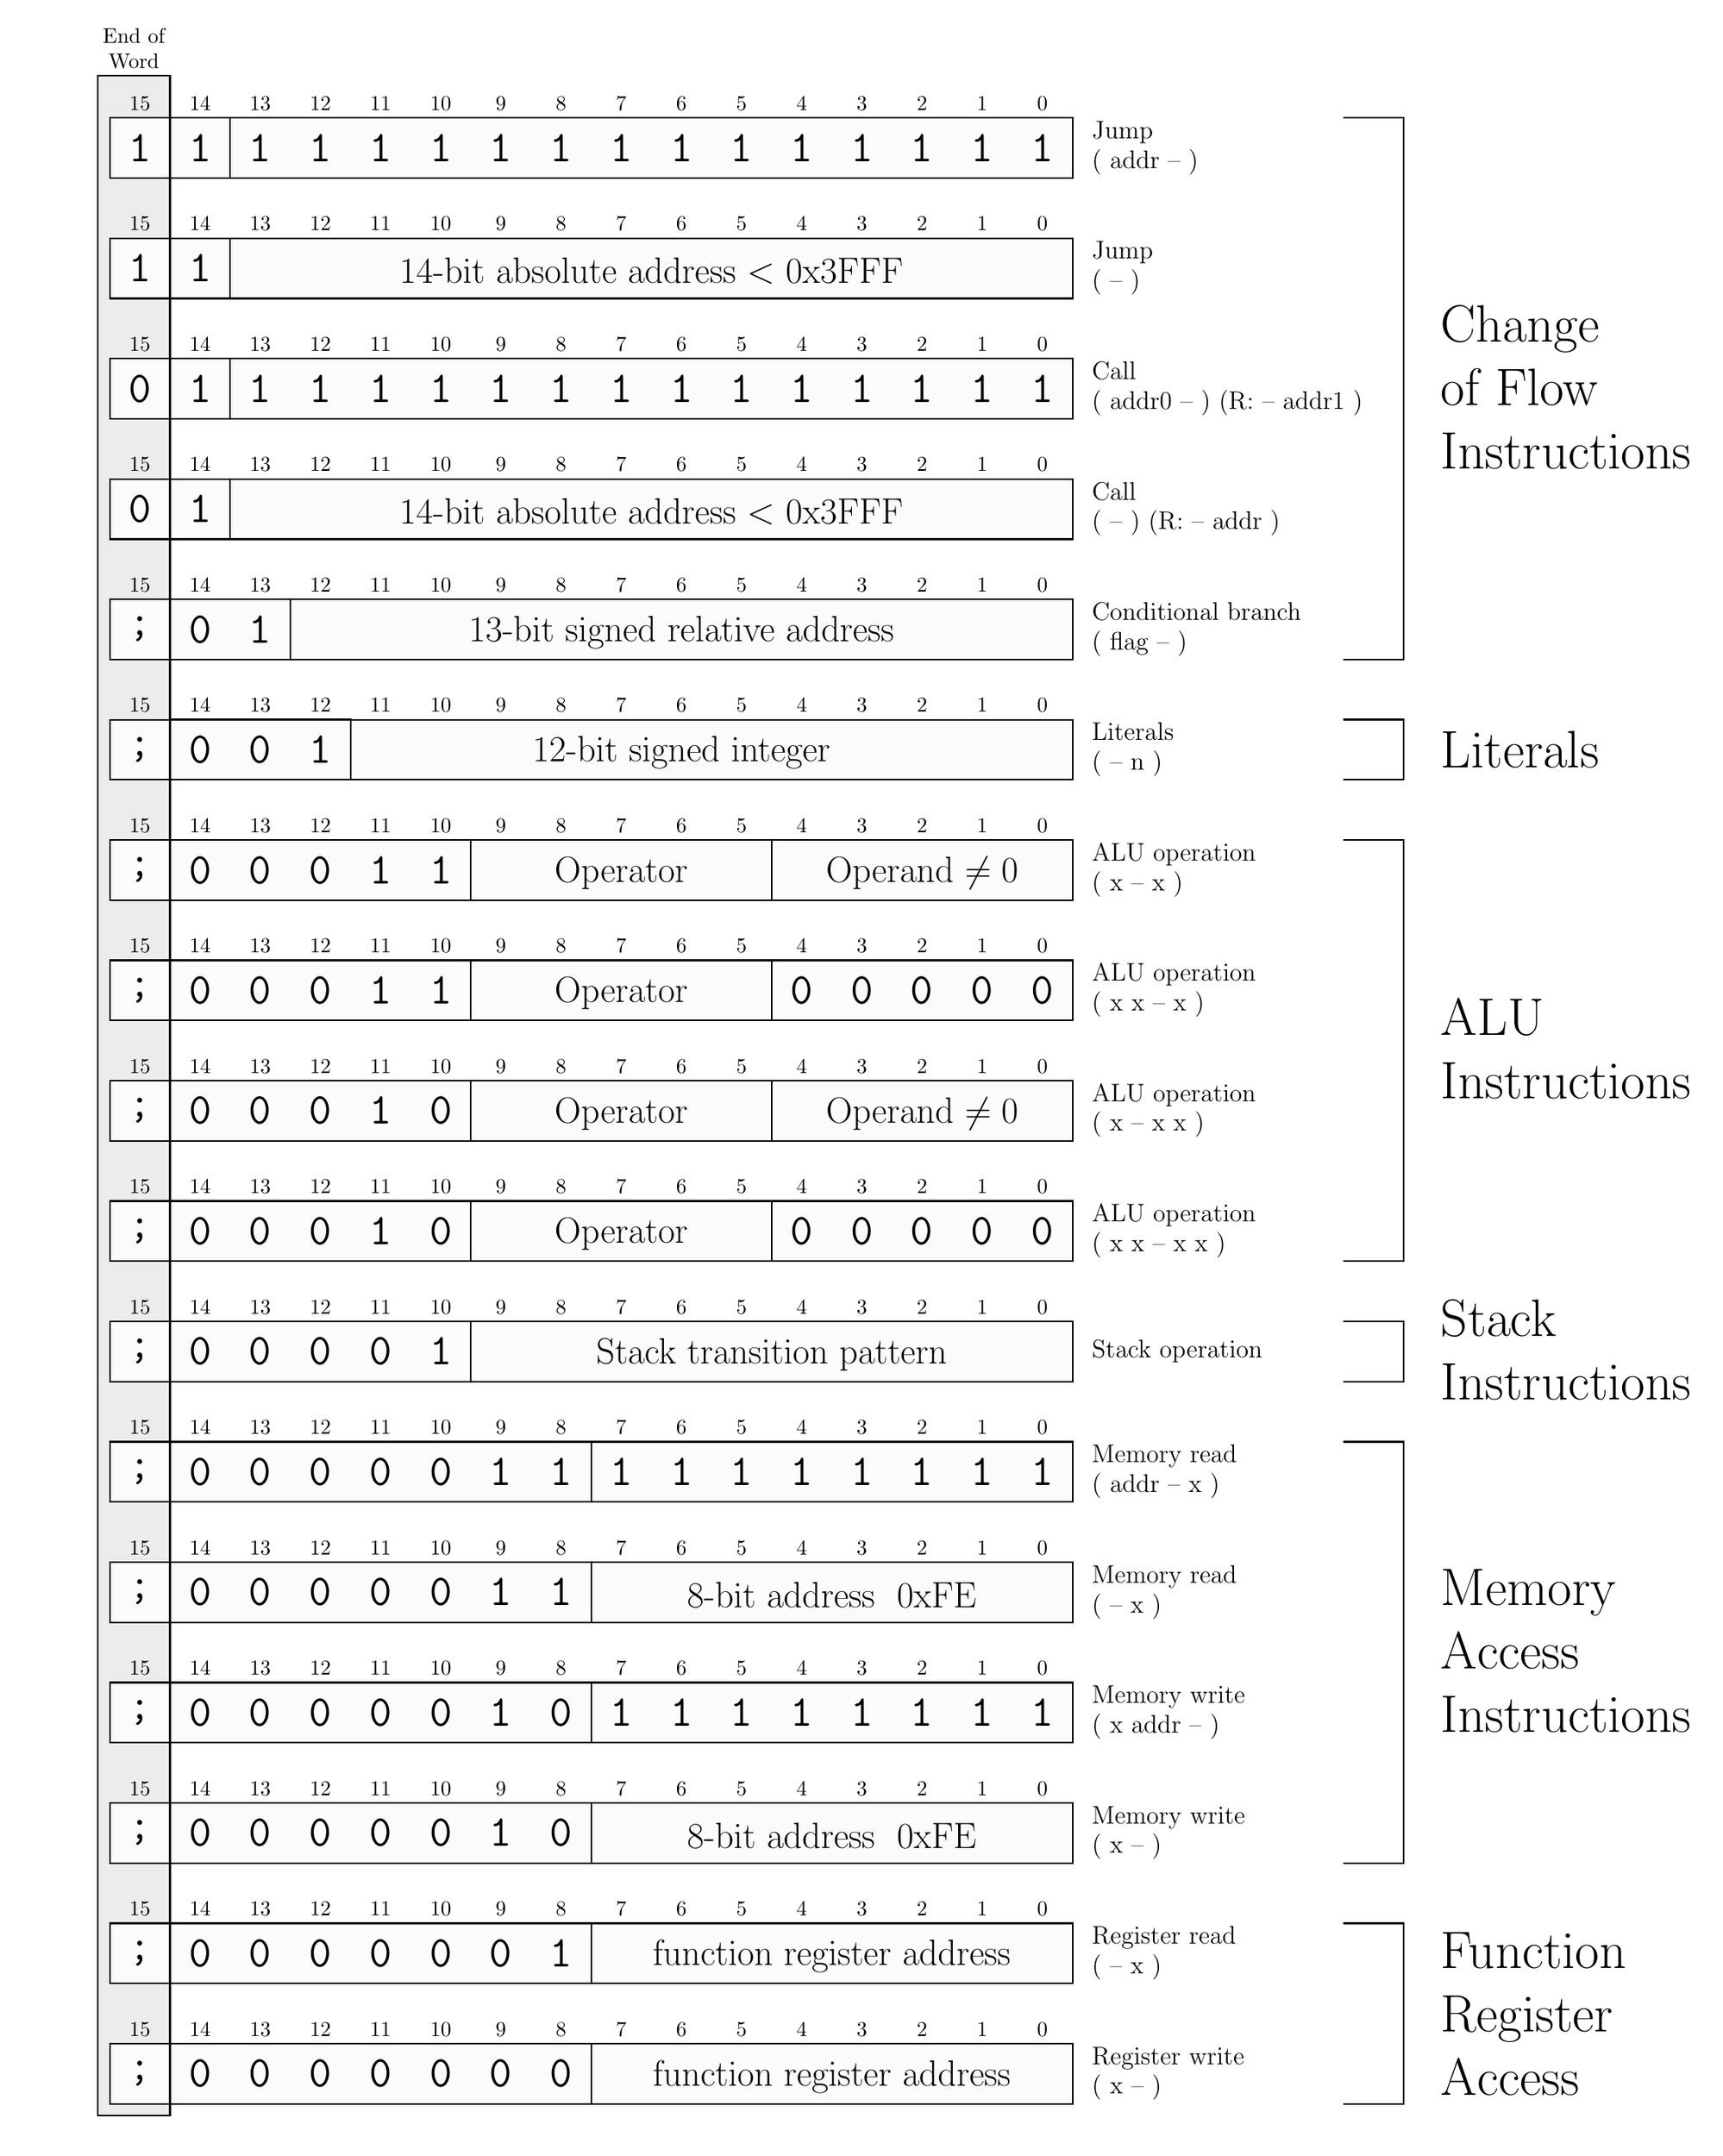
\begin{tikzpicture}
      
        %Instruction
        \newsavebox{\instruction}
        \savebox{\instruction}{
          \draw [thick, fill=gray!3] (0,0) rectangle (16,1);
          \draw [thick, fill=gray!3] (0,0) rectangle (1,1);
          \node [above] at (0.5,1)  {15};
          \node [above] at (1.5,1)  {14};
          \node [above] at (2.5,1)  {13};
          \node [above] at (3.5,1)  {12};
          \node [above] at (4.5,1)  {11};
          \node [above] at (5.5,1)  {10};
          \node [above] at (6.5,1)  {9};
          \node [above] at (7.5,1)  {8};
          \node [above] at (8.5,1)  {7};
          \node [above] at (9.5,1)  {6};
          \node [above] at (10.5,1) {5};
          \node [above] at (11.5,1) {4};
          \node [above] at (12.5,1) {3};
          \node [above] at (13.5,1) {2};
          \node [above] at (14.5,1) {1};
          \node [above] at (15.5,1) {0};
        };

        %Return bit
        \draw [thick, fill=gray!15] (0.8,0.3) rectangle (2,34.2);
        \node [above] at (1.4,34.2) {
          \begin{minipage}[c]{10em}
            \begin{center}
              End of\\
              Word
            \end{center}
          \end{minipage}};

        %Change of flow instructions
        \draw [thick] (21.5,33.5) -- (22.5,33.5) -- (22.5,24.5) -- (21.5,24.5);
        \node [right] at (23,28.5) {
          \begin{minipage}[l]{12em}
            \Huge{
              Change \\
              of Flow \\
              Instructions
            }
           \end{minipage}};

        %Jump
        \begin{scope}[shift={(1,32.5)}]
          \node at (0,0) {\usebox{\instruction}};
          \node         at (0.5,0.5)     {\huge{\texttt{1}}};
          \draw [thick] (1,0) rectangle  (2,1);
          \node         at (1.5,0.5)     {\huge{\texttt{1}}};
          \node         at (2.5,0.5)     {\huge{\texttt{1}}};
          \node         at (3.5,0.5)     {\huge{\texttt{1}}};
          \node         at (4.5,0.5)     {\huge{\texttt{1}}};
          \node         at (5.5,0.5)     {\huge{\texttt{1}}};
          \node         at (6.5,0.5)     {\huge{\texttt{1}}};
          \node         at (7.5,0.5)     {\huge{\texttt{1}}};
          \node         at (8.5,0.5)     {\huge{\texttt{1}}};
          \node         at (9.5,0.5)     {\huge{\texttt{1}}};
          \node         at (10.5,0.5)    {\huge{\texttt{1}}};
          \node         at (11.5,0.5)    {\huge{\texttt{1}}};
          \node         at (12.5,0.5)    {\huge{\texttt{1}}};
          \node         at (13.5,0.5)    {\huge{\texttt{1}}};
          \node         at (14.5,0.5)    {\huge{\texttt{1}}};
          \node         at (15.5,0.5)    {\huge{\texttt{1}}};
          \node [right] at (16.2,0.5) {
            \begin{minipage}[l]{14em}
              \large{
                Jump \\
                ( addr -- )
              }
          \end{minipage}};
        \end{scope}

        %Jump
        \begin{scope}[shift={(1,30.5)}]
          \node at (0,0) {\usebox{\instruction}};
          \node         at (0.5,0.5)     {\huge{\texttt{1}}};
          \draw [thick] (1,0) rectangle  (2,1);
          \node         at (1.5,0.5)     {\huge{\texttt{1}}};
          \node         at (9,0.45)      {\LARGE{14-bit absolute address $<$ 0x3FFF}};
          \node [right] at (16.2,0.5) {
            \begin{minipage}[l]{14em}
              \large{
                Jump \\
                ( -- )
              }
          \end{minipage}};
        \end{scope}

        %Call
        \begin{scope}[shift={(1,28.5)}]
          \node at (0,0) {\usebox{\instruction}};
          \node         at (0.5,0.5)     {\huge{\texttt{0}}};
          \draw [thick] (1,0) rectangle  (2,1);
          \node         at (1.5,0.5)     {\huge{\texttt{1}}};
          \node         at (2.5,0.5)     {\huge{\texttt{1}}};
          \node         at (3.5,0.5)     {\huge{\texttt{1}}};
          \node         at (4.5,0.5)     {\huge{\texttt{1}}};
          \node         at (5.5,0.5)     {\huge{\texttt{1}}};
          \node         at (6.5,0.5)     {\huge{\texttt{1}}};
          \node         at (7.5,0.5)     {\huge{\texttt{1}}};
          \node         at (8.5,0.5)     {\huge{\texttt{1}}};
          \node         at (9.5,0.5)     {\huge{\texttt{1}}};
          \node         at (10.5,0.5)    {\huge{\texttt{1}}};
          \node         at (11.5,0.5)    {\huge{\texttt{1}}};
          \node         at (12.5,0.5)    {\huge{\texttt{1}}};
          \node         at (13.5,0.5)    {\huge{\texttt{1}}};
          \node         at (14.5,0.5)    {\huge{\texttt{1}}};
          \node         at (15.5,0.5)    {\huge{\texttt{1}}};
          \node [right] at (16.2,0.5) {
            \begin{minipage}[l]{14em}
              \large{
                Call \\
                ( addr0 -- ) (R: -- addr1 )
              }
          \end{minipage}};
        \end{scope}

        %Call
        \begin{scope}[shift={(1,26.5)}]
          \node at (0,0) {\usebox{\instruction}};
          \node         at (0.5,0.5)     {\huge{\texttt{0}}};
          \draw [thick] (1,0) rectangle  (2,1);
          \node         at (1.5,0.5)     {\huge{\texttt{1}}};
          \node         at (9,0.45)      {\LARGE{14-bit absolute address $<$ 0x3FFF}};
          \node [right] at (16.2,0.5) {
            \begin{minipage}[l]{14em}
              \large{
                Call \\
                ( -- ) (R: -- addr )
              }
          \end{minipage}};
        \end{scope}

        %%Conditional Branch
        %\begin{scope}[shift={(1,26.5)}]
        %  \node at (0,0) {\usebox{\instruction}};
        %  \node         at (0.5,0.5)     {\huge{\texttt{;}}};
        %  \draw [thick] (1,0) rectangle  (3,1);
        %  \node         at (1.5,0.5)     {\huge{\texttt{0}}};
        %  \node         at (2.5,0.5)     {\huge{\texttt{1}}};
        %  \node         at (3.5,0.5)     {\huge{\texttt{1}}};
        %  \node         at (4.5,0.5)     {\huge{\texttt{1}}};
        %  \node         at (5.5,0.5)     {\huge{\texttt{1}}};
        %  \node         at (6.5,0.5)     {\huge{\texttt{1}}};
        %  \node         at (7.5,0.5)     {\huge{\texttt{1}}};
        %  \node         at (8.5,0.5)     {\huge{\texttt{1}}};
        %  \node         at (9.5,0.5)     {\huge{\texttt{1}}};
        %  \node         at (10.5,0.5)    {\huge{\texttt{1}}};
        %  \node         at (11.5,0.5)    {\huge{\texttt{1}}};
        %  \node         at (12.5,0.5)    {\huge{\texttt{1}}};
        %  \node         at (13.5,0.5)    {\huge{\texttt{1}}};
        %  \node         at (14.5,0.5)    {\huge{\texttt{1}}};
        %  \node         at (15.5,0.5)    {\huge{\texttt{1}}};
        %  \node [right] at (16.2,0.5) {
        %    \begin{minipage}[l]{14em}
        %      \large{
        %        Conditional branch \\
        %        ( flag addr -- )
        %      }
        %  \end{minipage}};
        %\end{scope}
        
        %Conditional Branch
        \begin{scope}[shift={(1,24.5)}]
          \node at (0,0) {\usebox{\instruction}};
          \node         at (0.5,0.5)     {\huge{\texttt{;}}};
          \draw [thick] (1,0) rectangle  (3,1);
          \node         at (1.5,0.5)     {\huge{\texttt{0}}};
          \node         at (2.5,0.5)     {\huge{\texttt{1}}};
          \node         at (9.5,0.45)    {\LARGE{13-bit signed relative address}};
          \node [right] at (16.2,0.5) {
            \begin{minipage}[l]{14em}
              \large{
                Conditional branch \\
               ( flag -- )
              }
          \end{minipage}};
        \end{scope}

        %Literal instructions
        \draw [thick] (21.5,22.5) -- (22.5,22.5) -- (22.5,23.5) -- (21.5,23.5);
        \node [right] at (23,23) {
          \begin{minipage}[l]{12em}
            \Huge{
              Literals
            }
           \end{minipage}};

        %Literal 
        \begin{scope}[shift={(1,22.5)}]
          \node at (0,0) {\usebox{\instruction}};
          \node         at (0.5,0.5)     {\huge{\texttt{;}}};
          \draw [thick] (1,0) rectangle  (4,1);
          \node         at (1.5,0.5)     {\huge{\texttt{0}}};
          \node         at (2.5,0.5)     {\huge{\texttt{0}}};
          \node         at (3.5,0.5)     {\huge{\texttt{1}}};
          \node         at (9.5,0.45)    {\LARGE{12-bit signed integer}};
          \node [right] at (16.2,0.5) {
            \begin{minipage}[l]{14em}
              \large{
                Literals \\
                ( -- n )
              }
          \end{minipage}};
        \end{scope}

        %ALU instructions
        \draw [thick] (21.5,21.5) -- (22.5,21.5) -- (22.5,14.5) -- (21.5,14.5);
        \node [right] at (23,17.5) {
          \begin{minipage}[l]{12em}
            \Huge{
              ALU \\
              Instructions
            }
          \end{minipage}};
  
        %ALU operation ( x -- x )
        \begin{scope}[shift={(1,20.5)}]
          \node at (0,0) {\usebox{\instruction}};
          \node         at (0.5,0.5)     {\huge{\texttt{;}}};
          \draw [thick] (1,0) rectangle  (6,1);
          \draw [thick] (6,0) rectangle (11,1); 
          \node         at (1.5,0.5)     {\huge{\texttt{0}}};
          \node         at (2.5,0.5)     {\huge{\texttt{0}}};
          \node         at (3.5,0.5)     {\huge{\texttt{0}}};
          \node         at (4.5,0.5)     {\huge{\texttt{1}}};
          \node         at (5.5,0.5)     {\huge{\texttt{1}}};
          \node         at (8.5,0.45)    {\LARGE{Operator}};
          \node         at (13.5,0.45)   {\LARGE{Operand $\neq 0$}};
          \node [right] at (16.2,0.5) {
            \begin{minipage}[l]{14em}
              \large{
                ALU operation \\
                ( x -- x )
              }
          \end{minipage}};
        \end{scope}

        %ALU operation ( x x -- x )
        \begin{scope}[shift={(1,18.5)}]
          \node at (0,0) {\usebox{\instruction}};
          \node         at (0.5,0.5)     {\huge{\texttt{;}}};
          \draw [thick] (1,0) rectangle  (6,1);
          \draw [thick] (6,0) rectangle (11,1); 
          \node         at (1.5,0.5)     {\huge{\texttt{0}}};
          \node         at (2.5,0.5)     {\huge{\texttt{0}}};
          \node         at (3.5,0.5)     {\huge{\texttt{0}}};
          \node         at (4.5,0.5)     {\huge{\texttt{1}}};
          \node         at (5.5,0.5)     {\huge{\texttt{1}}};
          \node         at (8.5,0.45)    {\LARGE{Operator}};
          \node         at (11.5,0.5)    {\huge{\texttt{0}}};   
          \node         at (12.5,0.5)    {\huge{\texttt{0}}};   
          \node         at (13.5,0.5)    {\huge{\texttt{0}}};   
          \node         at (14.5,0.5)    {\huge{\texttt{0}}};   
          \node         at (15.5,0.5)    {\huge{\texttt{0}}};   
          \node [right] at (16.2,0.5) {
            \begin{minipage}[l]{14em}
              \large{
                ALU operation \\
                ( x x -- x )
              }
          \end{minipage}};
        \end{scope}
               
        %ALU operation ( x -- x x )
        \begin{scope}[shift={(1,16.5)}]
          \node at (0,0) {\usebox{\instruction}};
          \node         at (0.5,0.5)     {\huge{\texttt{;}}};
          \draw [thick] (1,0) rectangle  (6,1);
          \draw [thick] (6,0) rectangle (11,1); 
          \node         at (1.5,0.5)     {\huge{\texttt{0}}};
          \node         at (2.5,0.5)     {\huge{\texttt{0}}};
          \node         at (3.5,0.5)     {\huge{\texttt{0}}};
          \node         at (4.5,0.5)     {\huge{\texttt{1}}};
          \node         at (5.5,0.5)     {\huge{\texttt{0}}};
          \node         at (8.5,0.45)    {\LARGE{Operator}};
          \node         at (13.5,0.45)   {\LARGE{Operand $\neq 0$}};
          \node [right] at (16.2,0.5) {
            \begin{minipage}[l]{14em}
              \large{
                ALU operation \\
                ( x -- x x )
              }
          \end{minipage}};
        \end{scope}

        %ALU operation ( x x -- x x )
        \begin{scope}[shift={(1,14.5)}]
          \node at (0,0) {\usebox{\instruction}};
          \node         at (0.5,0.5)     {\huge{\texttt{;}}};
          \draw [thick] (1,0) rectangle  (6,1);
          \draw [thick] (6,0) rectangle (11,1); 
          \node         at (1.5,0.5)     {\huge{\texttt{0}}};
          \node         at (2.5,0.5)     {\huge{\texttt{0}}};
          \node         at (3.5,0.5)     {\huge{\texttt{0}}};
          \node         at (4.5,0.5)     {\huge{\texttt{1}}};
          \node         at (5.5,0.5)     {\huge{\texttt{0}}};
          \node         at (8.5,0.45)    {\LARGE{Operator}};
          \node         at (11.5,0.5)    {\huge{\texttt{0}}};   
          \node         at (12.5,0.5)    {\huge{\texttt{0}}};   
          \node         at (13.5,0.5)    {\huge{\texttt{0}}};   
          \node         at (14.5,0.5)    {\huge{\texttt{0}}};   
          \node         at (15.5,0.5)    {\huge{\texttt{0}}};   
          \node [right] at (16.2,0.5) {
            \begin{minipage}[l]{14em}
              \large{
                ALU operation \\
                ( x x -- x x )
              }
          \end{minipage}};
        \end{scope}

        %Stack instructions
        \draw [thick] (21.5,12.5) -- (22.5,12.5) -- (22.5,13.5) -- (21.5,13.5);
        \node [right] at (23,12.5) {
          \begin{minipage}[l]{12em}
            \Huge{
              Stack \\
              Instructions
            }
           \end{minipage}};

        %Stack operation 
        \begin{scope}[shift={(1,12.5)}]
          \node at (0,0) {\usebox{\instruction}};
          \node         at (0.5,0.5)     {\huge{\texttt{;}}};
          \draw [thick] (1,0) rectangle (6,1); 
          \node         at (1.5,0.5)     {\huge{\texttt{0}}};
          \node         at (2.5,0.5)     {\huge{\texttt{0}}};
          \node         at (3.5,0.5)     {\huge{\texttt{0}}};
          \node         at (4.5,0.5)     {\huge{\texttt{0}}};   
          \node         at (5.5,0.5)     {\huge{\texttt{1}}};   
          \node         at (11,0.45)     {\LARGE{Stack transition pattern}};
          \node [right] at (16.2,0.5) {
            \begin{minipage}[l]{14em}
              \large{
                Stack operation
              }
          \end{minipage}};
        \end{scope}

        %Memory access instructions
        \draw [thick] (21.5,11.5) -- (22.5,11.5) -- (22.5,4.5) -- (21.5,4.5);
        \node [right] at (23,7.5) {
          \begin{minipage}[l]{12em}
            \Huge{
              Memory \\
              Access \\
              Instructions
            }
           \end{minipage}};

        %Memory read
        \begin{scope}[shift={(1,10.5)}]
          \node at (0,0) {\usebox{\instruction}};
          \node         at (0.5,0.5)     {\huge{\texttt{;}}};
          \draw [thick] (1,0) rectangle  (8,1);
          \node         at (1.5,0.5)     {\huge{\texttt{0}}};
          \node         at (2.5,0.5)     {\huge{\texttt{0}}};
          \node         at (3.5,0.5)     {\huge{\texttt{0}}};
          \node         at (4.5,0.5)     {\huge{\texttt{0}}};
          \node         at (5.5,0.5)     {\huge{\texttt{0}}};
          \node         at (6.5,0.5)     {\huge{\texttt{1}}};
          \node         at (7.5,0.5)     {\huge{\texttt{1}}};
          \node         at (8.5,0.5)     {\huge{\texttt{1}}};
          \node         at (9.5,0.5)     {\huge{\texttt{1}}};
          \node         at (10.5,0.5)    {\huge{\texttt{1}}};
          \node         at (11.5,0.5)    {\huge{\texttt{1}}};
          \node         at (12.5,0.5)    {\huge{\texttt{1}}};
          \node         at (13.5,0.5)    {\huge{\texttt{1}}};
          \node         at (14.5,0.5)    {\huge{\texttt{1}}};
          \node         at (15.5,0.5)    {\huge{\texttt{1}}};
          \node [right] at (16.2,0.5) {
           \begin{minipage}[l]{14em}
              \large{
                Memory read \\
                ( addr -- x )
              }
          \end{minipage}};
        \end{scope}

        %Memory read
        \begin{scope}[shift={(1,8.5)}]
          \node at (0,0) {\usebox{\instruction}};
          \node         at (0.5,0.5)     {\huge{\texttt{;}}};
          \draw [thick] (1,0) rectangle  (8,1);
          \node         at (1.5,0.5)     {\huge{\texttt{0}}};
          \node         at (2.5,0.5)     {\huge{\texttt{0}}};
          \node         at (3.5,0.5)     {\huge{\texttt{0}}};
          \node         at (4.5,0.5)     {\huge{\texttt{0}}};
          \node         at (5.5,0.5)     {\huge{\texttt{0}}};
          \node         at (6.5,0.5)     {\huge{\texttt{1}}};
          \node         at (7.5,0.5)     {\huge{\texttt{1}}};
          \node         at (12,0.45)    {\LARGE{8-bit address $\leqslant$ 0xFE}};
          \node [right] at (16.2,0.5) {
           \begin{minipage}[l]{14em}
              \large{
                Memory read \\
                ( -- x )
              }
          \end{minipage}};
        \end{scope}


        %Memory write
        \begin{scope}[shift={(1,6.5)}]
          \node at (0,0) {\usebox{\instruction}};
          \node         at (0.5,0.5)     {\huge{\texttt{;}}};
          \draw [thick] (1,0) rectangle  (8,1);
          \node         at (1.5,0.5)     {\huge{\texttt{0}}};
          \node         at (2.5,0.5)     {\huge{\texttt{0}}};
          \node         at (3.5,0.5)     {\huge{\texttt{0}}};
          \node         at (4.5,0.5)     {\huge{\texttt{0}}};
          \node         at (5.5,0.5)     {\huge{\texttt{0}}};
          \node         at (6.5,0.5)     {\huge{\texttt{1}}};
          \node         at (7.5,0.5)     {\huge{\texttt{0}}};
          \node         at (8.5,0.5)     {\huge{\texttt{1}}};
          \node         at (9.5,0.5)     {\huge{\texttt{1}}};
          \node         at (10.5,0.5)    {\huge{\texttt{1}}};
          \node         at (11.5,0.5)    {\huge{\texttt{1}}};
          \node         at (12.5,0.5)    {\huge{\texttt{1}}};
          \node         at (13.5,0.5)    {\huge{\texttt{1}}};
          \node         at (14.5,0.5)    {\huge{\texttt{1}}};
          \node         at (15.5,0.5)    {\huge{\texttt{1}}};
          \node [right] at (16.2,0.5) {
           \begin{minipage}[l]{14em}
              \large{
                Memory write \\
                ( x addr -- )
              }
          \end{minipage}};
        \end{scope}

        %Memory write
        \begin{scope}[shift={(1,4.5)}]
          \node at (0,0) {\usebox{\instruction}};
          \node         at (0.5,0.5)     {\huge{\texttt{;}}};
          \draw [thick] (1,0) rectangle  (8,1);
          \node         at (1.5,0.5)     {\huge{\texttt{0}}};
          \node         at (2.5,0.5)     {\huge{\texttt{0}}};
          \node         at (3.5,0.5)     {\huge{\texttt{0}}};
          \node         at (4.5,0.5)     {\huge{\texttt{0}}};
          \node         at (5.5,0.5)     {\huge{\texttt{0}}};
          \node         at (6.5,0.5)     {\huge{\texttt{1}}};
          \node         at (7.5,0.5)     {\huge{\texttt{0}}};
          \node         at (12,0.45)     {\LARGE{8-bit address $\leqslant$ 0xFE}};
          \node [right] at (16.2,0.5) {
           \begin{minipage}[l]{14em}
              \large{
                Memory write \\
                ( x -- )
              }
          \end{minipage}};
        \end{scope}

        %Function register access
        \draw [thick] (21.5,3.5) -- (22.5,3.5) -- (22.5,0.5) -- (21.5,0.5);
        \node [right] at (23,2) {
          \begin{minipage}[l]{12em}
            \Huge{
              Function \\
              Register \\
              Access
            }
           \end{minipage}};
       
        %Function register read
        \begin{scope}[shift={(1,2.5)}]
          \node at (0,0) {\usebox{\instruction}};
          \node         at (0.5,0.5)     {\huge{\texttt{;}}};
          \draw [thick] (1,0) rectangle  (8,1);
          \node         at (1.5,0.5)     {\huge{\texttt{0}}};
          \node         at (2.5,0.5)     {\huge{\texttt{0}}};
          \node         at (3.5,0.5)     {\huge{\texttt{0}}};
          \node         at (4.5,0.5)     {\huge{\texttt{0}}};
          \node         at (5.5,0.5)     {\huge{\texttt{0}}};
          \node         at (6.5,0.5)     {\huge{\texttt{0}}};
          \node         at (7.5,0.5)     {\huge{\texttt{1}}};
          \node         at (12,0.45)     {\LARGE{function register address}};
          \node [right] at (16.2,0.5) {
           \begin{minipage}[l]{14em}
              \large{
                Register read \\
                ( -- x )
              }
          \end{minipage}};
        \end{scope}

        %Function register write
        \begin{scope}[shift={(1,0.5)}]
          \node at (0,0) {\usebox{\instruction}};
          \node         at (0.5,0.5)     {\huge{\texttt{;}}};
          \draw [thick] (1,0) rectangle  (8,1);
          \node         at (1.5,0.5)     {\huge{\texttt{0}}};
          \node         at (2.5,0.5)     {\huge{\texttt{0}}};
          \node         at (3.5,0.5)     {\huge{\texttt{0}}};
          \node         at (4.5,0.5)     {\huge{\texttt{0}}};
          \node         at (5.5,0.5)     {\huge{\texttt{0}}};
          \node         at (6.5,0.5)     {\huge{\texttt{0}}};
          \node         at (7.5,0.5)     {\huge{\texttt{0}}};
          \node         at (12,0.45)     {\LARGE{function register address}};
          \node [right] at (16.2,0.5) {
           \begin{minipage}[l]{14em}
              \large{
                Register write  \\
                ( x -- )
              }
          \end{minipage}};
        \end{scope}
        
      \end{tikzpicture}
    }
  }
  \caption{Instruction encoding}
  \label{opcodes:encoding}
  %\end{center}
\end{figure}

\subsection{Return from a Call (\texttt{;})}
\label{opcodes:rtc}

Rather than  providing a dedicated instruction to end the execution of 
word in Forth and to return the caller's program flow, the N1 allows
to perform this operation in parallel to the execution of any of its
instructions. Each \gls{opcode} contains a bit (bit 15) to indicate, that the
current instruction is the last operation of the current word. If this bit
is set, the program flow will resume at the calling word as soon as the
operationis performed.

As shown in \figref{opcodes:encoding}, bit 15 is also distinction between the
encoding of \gls{jump} and of \gls{call} instructions.
Considering that the last \gls{call} in a word definition can be optimized
to a \gls{jump}, bit 15 can be regarded
as the termination bit for \gls{call} instructions as well.

For a Forth compiler, this means that the semi-colon (\texttt{\gls{semicolon}})
always translates to setting bit 15 of the last instruction.

\subsection{Jump Instructions}
\label{opcodes:jump}

\Gls{jump} instructions transfer the program flow to any address
location within the supported 128KB program space. \Gls{jump} instructions consume an absolute
destination address which can either be placed on the top of the \gls{ps} or encoded
into the opcode of the instruction (only for destination addresses $<$ 0x3FFF).

\subsection{Call Instructions}
\label{opcodes:call}

\Gls{call} instructions temporarily transfer the program flow to any address
location within the supported 128KB program space, while pushing a return address onto
the \gls{rs}. \Gls{call} instructions consume an absolute
destination address which can either be placed on the top of the \Gls{ps} or encoded
into the opcode of the instruction (only for destination addresses $<$ 0x3FFF).

\subsection{Conditional Branches}
\label{opcodes:branch}

\Glspl{branch} invoke a change of program flow depending on the argument at the \glslink{tos}{top}
of the \gls{ps}.
If it is zero, then the branch is taken.
The branch destination is a \glslink{reladr}{relative address}, encoded into the opcode
of the instruction in the range of $\pm$ 8KB.
A relative address of value zero points to the istruction following the \glspl{branch}.

\subsection{Literals}
\label{opcodes:literal}

Signed integer \glspl{literal} of 12-bit length can be pushed onto the \gls{ps} within
a single instruction. For larger integers a supplemental \gls{alu} instruction is required.
(see encoding \texttt{11100} in \tabref{opcodes:alu:operators})

\subsection{ALU Instructions}
\label{opcodes:alu}
\Gls{alu} instructions perform an operation on two \gls{cell} values, resulting in a new double 
\gls{cell} value. The result can either be placed entirely onto the \gls{ps}, or truncated, discarding
the most significant \gls{cell}. The first operand is always taken from the \gls{ps}. The second operand can
either be taken from the \gls{ps} or encoded into the opcode of the instruction. In the latter case,
the interpretation of the embedded 5-bit value depends on the operation. The \glslink{immop}{immediate} value is
interpreted as either an unsigned ($uimm$), a sign extended ($simm$), or an offsetted ($oimm$) integer value:

\begin{align*}
  uimm &= \text{opcode[4:0]}                                     \\
  simm &= \begin{cases}
            \text{opcode[4:0]},      &\text{if opcode[4:0]} < 16 \\
            \text{opcode[4:0]} - 32, &\text{if opcode[4:0]} \ge 16
          \end{cases}                                            \\
  oimm &= \text{opcode[4:0]} - 16
\end{align*}

\tabref{opcodes:alu:operators} lists the supported \gls{alu} operations.

\begingroup
\setlength{\LTleft}{-20cm plus -1fill}
\setlength{\LTright}{\LTleft}
\begin{center}
  \rowcolors{1}{gray!12}{white}                                         %set alternating row color
  \begin{longtable}{|c|c|c|c|}
    \rowcolor{white}
    \caption{\Gls{alu} operations}
    \label{opcodes:alu:operators} \\
    %Header
    \hline                                     
    \rowcolor{gray!25}
    \multicolumn{1}{|c|}{\textbf{\rule{0pt}{2.5ex}Encoding}}     &  
    \multicolumn{1}{c|}{\textbf{\rule{0pt}{2.5ex}Operation}}     &
    \multicolumn{1}{c|}{\textbf{\rule{0pt}{2.5ex}( x1 -- d )}}   &
    \multicolumn{1}{c|}{\textbf{\rule{0pt}{2.5ex}( x1 x2 -- d ) }} \\
    \hline
    \endhead                               
    %Footers
    \hline
    \rowcolor{white}
    \multicolumn{4}{r}{\tiny{...continued}} \\
    \endfoot
    \hline
    \endlastfoot

    %Adder operations
    %---------------------------------
    %Sum
    \texttt{00000}                       &
    Sum                                  &
    $uimm$ $+$ x1                        &
    x1 $+$ x2                            \\ \hline
    
    %Sum
    \texttt{00001}                       &
    Absolute value                       &
    $oimm$ $+$ ABS(x1)                   &
    x1 $+$ ABS(x2)                       \\ \hline
                                           
    %Difference                            
    \texttt{00010}                       &
    Difference                           &
    x1 $-$ $uimm$                        &
    x2 $-$ x1                            \\ \hline

    %Difference                            
    \texttt{00011}                       &
    Difference                           &
    $oimm$ $-$ x1                        &
    x1 $-$ x2                            \\ \hline
    %---------------------------------
    
    %MAX/MIN values
    %---------------------------------
    %Unsigned MIN value
    \texttt{00100}                       &
    Unsigned minimum value               &
    UMIN($uimm$, x1)                     &
    UMIN(x1, x2)                         \\ \hline
    
    %Signed MAX value
    \texttt{00101}                       &
    Signed maximum value                 &
    MAX($oimm$, x1)                      &
    MAX(x1, x2)                          \\ \hline
                                           
    %Unsigned MAX value                            
    \texttt{00110}                       &
    Unsigned maximum value               &
    UMAX($uimm$, x1)                     &
    UMAX(x1, x2)                         \\ \hline

    %Signed MIN value                            
    \texttt{00111}                       &
    Signed minimum value                 &
    MIN($oimm$, x1)                      &
    MIN(x1, x2)                          \\ \hline
    %---------------------------------

    %Equals comparisons
    %---------------------------------
    %Equals                    
    \texttt{01000}                       &
    Equals comparison                    &
    $uimm$ $=$ x1?                       &
    x1 $=$ x2?                           \\ \hline

    %Equals
    \texttt{01001}                       &
    Equals comparison                    &
    $oimm$ $=$ x1?                       &
    x1 $=$ x2?                           \\ \hline

    %Not-Equals                     
    \texttt{01010}                       &
    Not-equals comparison                &
    $uimm$ $\ne$ x1?                     &
    x1 $\ne$ x2?                         \\ \hline

    %Not-Eqials
    \texttt{01011}                       &
    Not-equals comparison                &
    $oimm$ $\ne$ x1?                     &
    x1 $\ne$ x2?                         \\ \hline
    %---------------------------------

    %Greater/lower-than comparisons
    %---------------------------------
    %Unsigned greater-than                     
    \texttt{01100}                       &
    Unsigned greater-than comparison     &
    $uimm$ $>$ x1?                       &
    x1 $>$ x2?                           \\ \hline

    %Signed lower-than
    \texttt{01101}                       &
    Signed lower-than comparison         &
    $oimm$ $<$ x1?                       &
    x1 $<$ x2?                           \\ \hline

    %Unsigned lower-than                     
    \texttt{01110}                       &
    Unsigned lower-than comparison       &
    $uimm$ $<$ x1?                       &
    x1 $<$ x2?                           \\ \hline

    %Signed greater-than
    \texttt{01111}                       &
    Signed greater-than                  &
    $oimm$ $>$ x1?                       &
    x1 $>$ x2?                           \\ \hline
    %---------------------------------
      
    %Multiplier operations             
    %---------------------------------
    %Unsigned product                  
      \texttt{10000}                     &
      Unsigned product                   &
      $uimm$ $*$ x1                      &
      x1 $*$ x2                          \\ \hline
                                         
    %Unsigned product                      
      \texttt{10001}                     &
      Unsigned product                   &
      $simm$ $*$ x1                      &
      x1 $*$ x2                          \\ \hline
                                         
    %Signed product                  
      \texttt{10010}                     &
      Signed product                     &
      $uimm$ $*$ x1                      &
      x1 $*$ x2                          \\ \hline
                                         
    %Signed product                      
      \texttt{10011}                     &
      Signed product                     &
      $simm$ $*$ x1                      &
      x1 $*$ x2                          \\ \hline
    %---------------------------------
                                         
    %Bitwise logic operations          
    %---------------------------------
   %AND                               
      \texttt{10100}                     &
      Logic AND                          &
      $simm$ $\land$ x1                  &
      x1 $\land$ x2                      \\ \hline
                                         
    %XOR                                 
      \texttt{10101}                     &
      Logic XOR                          &
      $simm$ $\oplus$ x1                 &
      x1 $\oplus$ x2                     \\ \hline
                                         
    %OR                                  
      \texttt{10110}                     &
      Logic OR                           &
      $uimm$ $\lor$ x1                   &
      x1 $\lor$ x2                       \\ \hline
                                         
    %Reserved                            
      \texttt{10111}                     &
      \multicolumn{3}{c|}{Reserved}      \\ \hline
    %---------------------------------

    %Shift operations             
    %---------------------------------
    %Logic right shift
      \texttt{11000}                     &
      Logic right shift                  &
      x1 $\gg$ $uimm$                    &
      x1 $\gg$ x2                        \\ \hline
                                         
    %Logic left shift                    
      \texttt{11001}                     &
      Logic left shift                   &
      x1 $\ll$ $uimm$                    &
      x1 $\ll$ x2                        \\ \hline
                                         
    %Arithmetic right shift              
      \texttt{11010}                     &                      
      Arithmetic right shift             &
      x1 $\gg$ $uimm$                    &
      x1 $\gg$ x2                        \\ \hline

    %Reserved                          
      \texttt{11011}                     &
      \multicolumn{3}{c|}{Reserved}      \\ \hline
    %---------------------------------

    %Special operations             
    %---------------------------------
    %Literal value
      \texttt{11100}                     &
      Set upper bits of a literal value  &
      {$simm$, x1[11:0]}                 &   
      {$simm$, x2[11:0]}                 \\ \hline
 
    %Reserved                          
      \texttt{11101}                     &
      \multicolumn{3}{c|}{Reserved}      \\ \hline


    %Reserved                          
      \texttt{11110}                     &
      \multicolumn{3}{c|}{Reserved}      \\ \hline

    %Reserved                          
      \texttt{11111}                     &
      \multicolumn{3}{c|}{Reserved}      \\ \hline
    %---------------------------------
    
  \end{longtable}
\end{center}  
\endgroup

\subsection{Stack Instructions}
\label{opcodes:stack}

The N1's stack instruction aims at efficiently implementing common stack operations
of the \Gls{forth} language, while only implementing the essential data paths, which are
needed for plain push and pull operations.

The opcode of the stack instruction contains a 10-bit field to specify a transition
pattern of the upper \glspl{cell} of the \gls{ps} and the \gls{rs}. 
The structure transition pattern is shown in \figref{opcodes:stack:transpat}.
    
\begin{figure}[!h]
  %\begin{center}
  \makebox[\textwidth][c]{
    \scalebox{0.8} {
      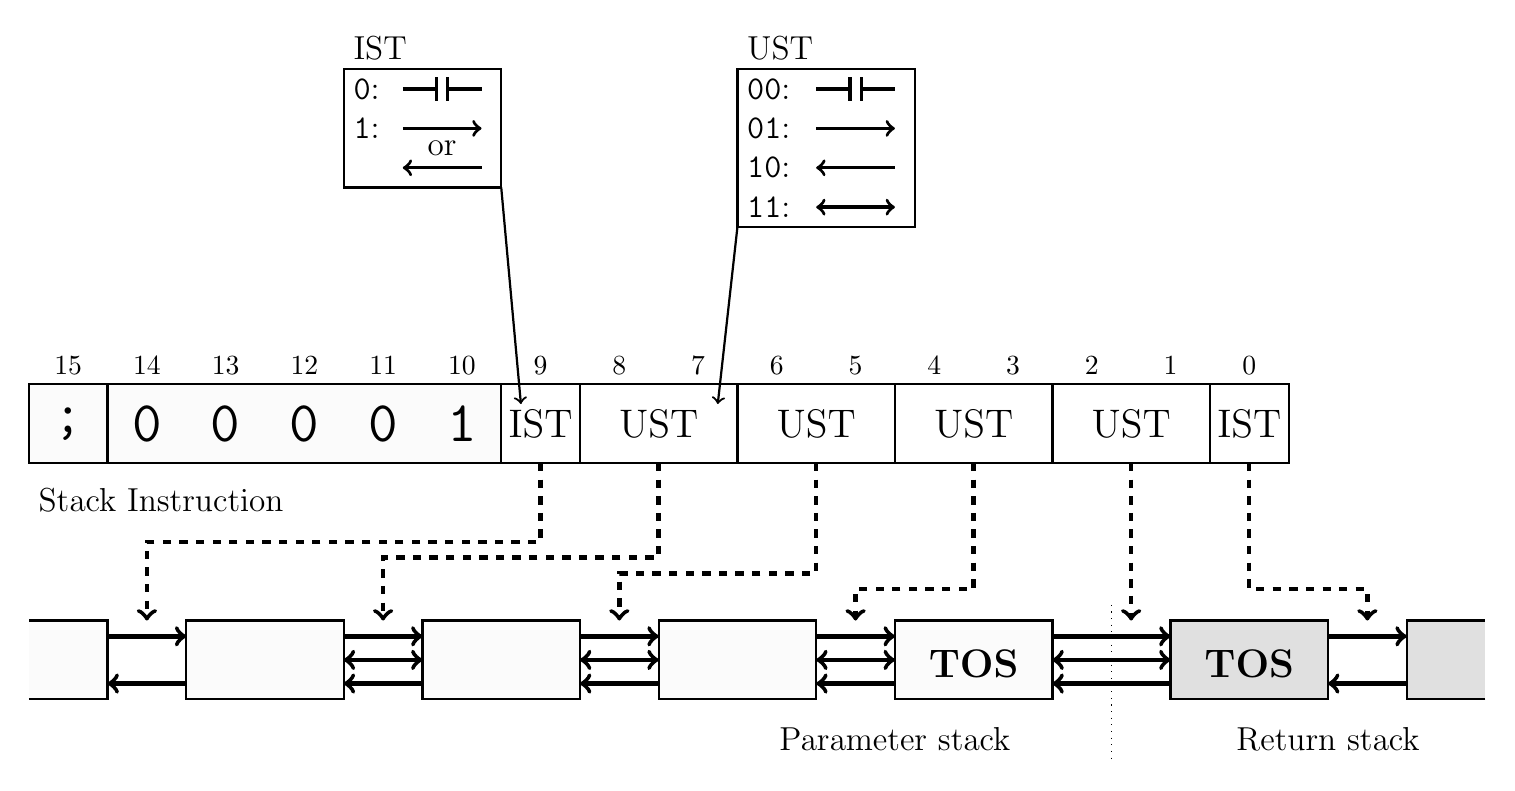
\begin{tikzpicture}

        %Stack instruction
        \draw [thick, fill=gray!3]  (1,4) rectangle (17,5);
        \draw [thick]               (1,4) rectangle  (2,5);
        \draw [thick]               (2,4) rectangle  (7,5); 
        \draw [thick, fill=white]   (7,4) rectangle  (8,5); 
        \draw [thick, fill=white]   (8,4) rectangle (10,5); 
        \draw [thick, fill=white]  (10,4) rectangle (12,5); 
        \draw [thick, fill=white]  (12,4) rectangle (14,5); 
        \draw [thick, fill=white]  (14,4) rectangle (16,5); 
        \draw [thick, fill=white]  (16,4) rectangle (17,5); 
  
        \node [above] at  (1.5,5) {15};
        \node [above] at  (2.5,5) {14};
        \node [above] at  (3.5,5) {13};
        \node [above] at  (4.5,5) {12};
        \node [above] at  (5.5,5) {11};
        \node [above] at  (6.5,5) {10};
        \node [above] at  (7.5,5) {9};
        \node [above] at  (8.5,5) {8};
        \node [above] at  (9.5,5) {7};
        \node [above] at (10.5,5) {6};
        \node [above] at (11.5,5) {5};
        \node [above] at (12.5,5) {4};
        \node [above] at (13.5,5) {3};
        \node [above] at (14.5,5) {2};
        \node [above] at (15.5,5) {1};
        \node [above] at (16.5,5) {0};

        \node         at (1.5,4.5)     {\huge{\texttt{;}}};
        \node         at (2.5,4.5)     {\huge{\texttt{0}}};
        \node         at (3.5,4.5)     {\huge{\texttt{0}}};
        \node         at (4.5,4.5)     {\huge{\texttt{0}}};
        \node         at (5.5,4.5)     {\huge{\texttt{0}}};   
        \node         at (6.5,4.5)     {\huge{\texttt{1}}};   

        \node         at (7.5,4.5)     {\Large{IST}};   
        \node         at (9,4.5)       {\Large{UST}};   
        \node         at (11,4.5)      {\Large{UST}};   
        \node         at (13,4.5)      {\Large{UST}};   
        \node         at (15,4.5)      {\Large{UST}};   
        \node         at (16.5,4.5)    {\Large{IST}};   
        
        \node [below right] at (1,3.8) {\large{Stack Instruction}};

        %IST field description
        \draw [thick]               (5,7.5) rectangle (7,9);
        \node [above right] at      (5,9) {\large{IST}};
        \node [right] at (5,8.75)    {\large{\texttt{0}:}};   
        \node [right] at (5,8.25)    {\large{\texttt{1}:}};

        \draw [very thick, -|]     (5.75,8.75)  -- (6.2,8.75);
        \draw [very thick, |-]     (6.3,8.75)   -- (6.75,8.75);
        \draw [very thick, ->]     (5.75,8.25)  -- (6.75,8.25);
        \node at (6.25,8)          {\large{or}};
        \draw [very thick, <-]     (5.75,7.75)  -- (6.75,7.75);         
        \draw [thick, ->]          (7,7.5)   --  (7.25,4.75);
       
        %UST field description
        \draw [thick]               (10,7) rectangle  (12.25,9);
        \node [above right] at      (10,9) {\large{UST}};
        \node [right] at (10,8.75) {\large{\texttt{00}:}};   
        \node [right] at (10,8.25) {\large{\texttt{01}:}};   
        \node [right] at (10,7.75) {\large{\texttt{10}:}};   
        \node [right] at (10,7.25) {\large{\texttt{11}:}};   

        \draw [very thick, -|]     (11,8.75)    -- (11.45,8.75);
        \draw [very thick, |-]     (11.55,8.75) -- (12,8.75);
        \draw [very thick, ->]     (11,8.25)    --  (12,8.25);
        \draw [very thick, <-]     (11,7.75)    --  (12,7.75);
        \draw [very thick, <->]    (11,7.25)    --  (12,7.25);         
        \draw [thick, ->]          (10,7)       --  (9.75,4.75);

        %Bit field association
        \draw [ultra thick, dashed, ->]  (7.5,4)  -- (7.5,3)    -- (2.5,3)    -- (2.5,2);
        \draw [ultra thick, dashed, ->]  (9,4)    -- (9,2.8)    -- (5.5,2.8)  -- (5.5,2);
        \draw [ultra thick, dashed, ->]  (11,4)   -- (11,2.6)   -- (8.5,2.6)  -- (8.5,2);
        \draw [ultra thick, dashed, ->]  (13,4)   -- (13,2.4)   -- (11.5,2.4) -- (11.5,2);
        \draw [ultra thick, dashed, ->]  (15,4)   -- (15,2);
        \draw [ultra thick, dashed, ->]  (16.5,4) -- (16.5,2.4) -- (18,2.4) -- (18,2);
    
        %Lower parameter stack
        \draw [thick, fill=gray!3]  (1,1) -- (2,1) -- (2,2) -- (1,2);
        \draw [ultra thick, ->]     (2,1.8) --  (3,1.8);
        \draw [ultra thick, <-]     (2,1.2) --  (3,1.2);         
       
        %Upper parameter stack
        \draw [thick, fill=gray!3]  (3,1) rectangle  (5,2);
        \draw [ultra thick, ->]     (5,1.8) --  (6,1.8);
        \draw [ultra thick, <->]    (5,1.5) --  (6,1.5);
        \draw [ultra thick, <-]     (5,1.2) --  (6,1.2);         

        \draw [thick, fill=gray!3]  (6,1) rectangle  (8,2);
        \draw [ultra thick, ->]     (8,1.8) --  (9,1.8);
        \draw [ultra thick, <->]    (8,1.5) --  (9,1.5);
        \draw [ultra thick, <-]     (8,1.2) --  (9,1.2);         

        \draw [thick, fill=gray!3]  (9,1) rectangle  (11,2);
        \draw [ultra thick, ->]     (11,1.8) --  (12,1.8);
        \draw [ultra thick, <->]    (11,1.5) --  (12,1.5);
        \draw [ultra thick, <-]     (11,1.2) --  (12,1.2);         

        \draw [thick, fill=gray!3]  (12,1) rectangle  (14,2);
        \node at (13,1.45)          {\Large{\textbf{TOS}}};        
        \node at (12,0.5)          {\large{Parameter stack}};
               
        %Stack boundary
        \draw [ultra thick, ->]     (14,1.8)    --  (15.5,1.8);
        \draw [ultra thick, <->]    (14,1.5)    --  (15.5,1.5);
        \draw [ultra thick, <-]     (14,1.2)    --  (15.5,1.2);         
        \draw [dotted]              (14.75,2.2) --  (14.75,0.2);

        %Upper return stack
        \draw [thick, fill=gray!24] (15.5,1) rectangle  (17.5,2);
        \node at (16.5,1.45)        {\Large{\textbf{TOS}}};
        \draw [ultra thick, ->]     (17.5,1.8) --  (18.5,1.8);
        \draw [ultra thick, <-]     (17.5,1.2) --  (18.5,1.2);         
        \node at (17.5,0.5)         {\large{Return stack}};

        %Lower return stack
        \draw [thick, fill=gray!24] (19.5,1) -- (18.5,1) -- (18.5,2) -- (19.5,2);
        
      \end{tikzpicture}
    }
  }
  \caption{Transition encoding of stack instructions}
  \label{opcodes:stack:transpat}
  %\end{center}
\end{figure}

The stack instruction contains four \gls{ust} fields which control the data movement within
the upper four \glspl{cell} of the \gls{ps} and the top \gls{cell} of the \gls{rs}. Each
\gls{ust} field determines the direction of data transfer between two neighboring stack
\glspl{cell}. Four options are selectable:
\begin{itemize}
  \item No data transfer
  \item Data transfer upwards (or towards the \gls{rs})
  \item Data transfer downwards (or towards the \gls{ps})
  \item Data exchange between two stack \glspl{cell}
\end{itemize}
It is possible to put the \gls{ust} fields into a combination which would trigger a data transfer of two
source \glspl{cell} to a single desination \gls{cell}.  
These combinations are reserved for instruction set extensions (see \secref{extensions}).
If no related instuction set extension is implemented, the outcome of these stack operations is undefined. 
In practice, the resulting data in the desination \gls{cell} is then a logic OR of all sources.

\begin{samepage}
The two remaining \gls{ist} fields in the stack instruction control the data movement of the \glspl{ls}.
Two options are selectable:
\begin{itemize}
  \item No data transfer
  \item Data shift throughout the entire \gls{is}. The direction is determined by the data movement of the lowest
        cell of the \gls{us} (see  \figref{opcodes:stack:istrans}).
\end{itemize}

\begin{figure}[!h]
  %\begin{center}
  \makebox[\textwidth][c]{
    \scalebox{0.4} {
      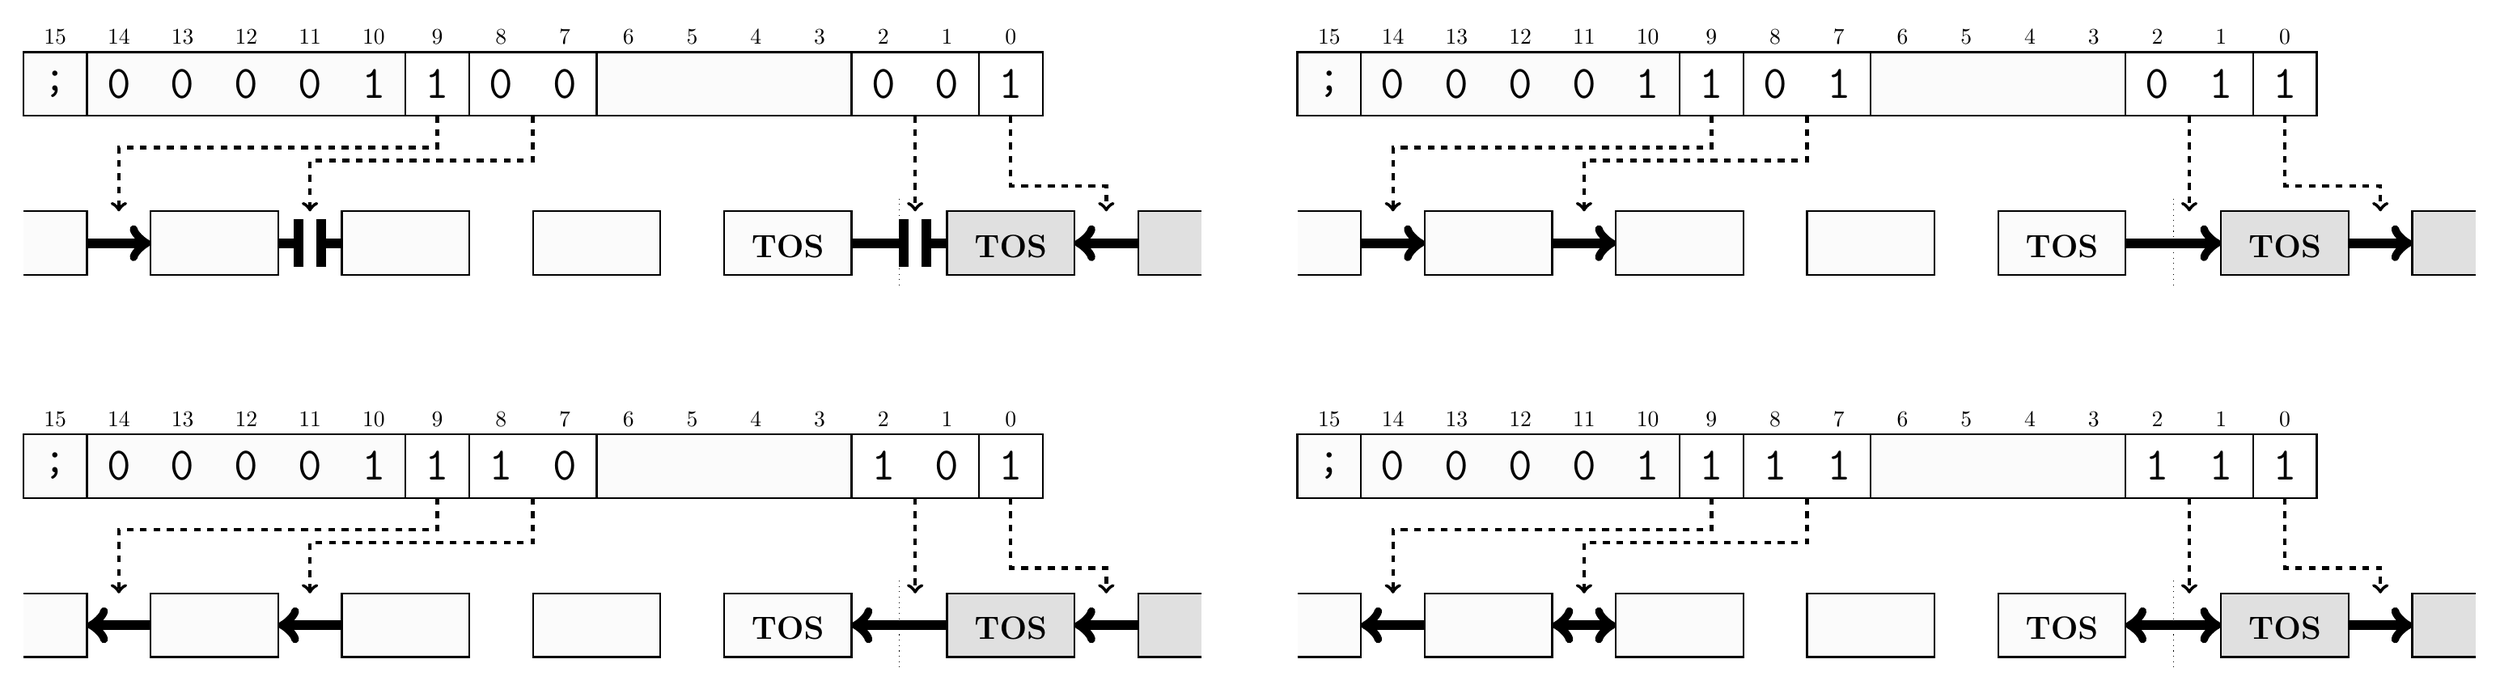
\begin{tikzpicture}
        %UST=00
         \begin{scope}[shift={(0,0)}]  
           %Stack instruction
           \draw [thick, fill=gray!3]  (1,3.5) rectangle (17,4.5);
           \draw [thick]               (1,3.5) rectangle  (2,4.5);
           \draw [thick]               (2,3.5) rectangle  (7,4.5); 
           \draw [thick, fill=white]   (7,3.5) rectangle  (8,4.5); 
           \draw [thick, fill=white]   (8,3.5) rectangle (10,4.5); 
           \draw [thick]               (10,3.5) rectangle (14,4.5); 
           %\draw [thick, fill=white]  (12,3.5) rectangle (14,4.5); 
           \draw [thick, fill=white]  (14,3.5) rectangle (16,4.5); 
           \draw [thick, fill=white]  (16,3.5) rectangle (17,4.5); 
           
           \node [above] at  (1.5,4.5) {15};
           \node [above] at  (2.5,4.5) {14};
           \node [above] at  (3.5,4.5) {13};
           \node [above] at  (4.5,4.5) {12};
           \node [above] at  (5.5,4.5) {11};
           \node [above] at  (6.5,4.5) {10};
           \node [above] at  (7.5,4.5) {9};
           \node [above] at  (8.5,4.5) {8};
           \node [above] at  (9.5,4.5) {7};
           \node [above] at (10.5,4.5) {6};
           \node [above] at (11.5,4.5) {5};
           \node [above] at (12.5,4.5) {4};
           \node [above] at (13.5,4.5) {3};
           \node [above] at (14.5,4.5) {2};
           \node [above] at (15.5,4.5) {1};
           \node [above] at (16.5,4.5) {0};
           
           \node         at (1.5,4)     {\huge{\texttt{;}}};
           \node         at (2.5,4)     {\huge{\texttt{0}}};
           \node         at (3.5,4)     {\huge{\texttt{0}}};
           \node         at (4.5,4)     {\huge{\texttt{0}}};
           \node         at (5.5,4)     {\huge{\texttt{0}}};   
           \node         at (6.5,4)     {\huge{\texttt{1}}};   
           
           \node         at (7.5,4)     {\huge{\texttt{1}}};   
           \node         at (8.5,4)     {\huge{\texttt{0}}};   
           \node         at (9.5,4)     {\huge{\texttt{0}}};   
           \node         at (14.5,4)    {\huge{\texttt{0}}};   
           \node         at (15.5,4)    {\huge{\texttt{0}}};   
           \node         at (16.5,4)    {\huge{\texttt{1}}};   
           
           %Bit field association
           \draw [ultra thick, dashed, ->]  (7.5,3.5)  -- (7.5,3)    -- (2.5,3)    -- (2.5,2);
           \draw [ultra thick, dashed, ->]  (9,3.5)    -- (9,2.8)    -- (5.5,2.8)  -- (5.5,2);
           \draw [ultra thick, dashed, ->]  (15,3.5)   -- (15,2);
           \draw [ultra thick, dashed, ->]  (16.5,3.5) -- (16.5,2.4) -- (18,2.4) -- (18,2);
           
           %Lower parameter stack
           \draw [thick, fill=gray!3]  (1,1) -- (2,1) -- (2,2) -- (1,2);
           \draw [line width=1ex, ->]  (2,1.5) --  (3,1.5);
           
           %Upper parameter stack
           \draw [thick, fill=gray!3]  (3,1) rectangle  (5,2);
           %\draw [line width=1ex, <->] (5,1.5) --  (6,1.5);
           \draw [line width=1ex, -|]     (5,1.5)  -- (5.4,1.5);
           \draw [line width=1ex, |-]     (5.6,1.5)   -- (6,1.5);
           
           \draw [thick, fill=gray!3]  (6,1) rectangle  (8,2);
           \draw [thick, fill=gray!3]  (9,1) rectangle  (11,2);
           \draw [thick, fill=gray!3]  (12,1) rectangle  (14,2);
           \node at (13,1.45)          {\Large{\textbf{TOS}}};        
                  
           %Stack boundary
           %\draw [line width=1ex, <->] (14,1.5)    --  (15.5,1.5);
           \draw [line width=1ex, -|]     (14,1.5) -- (14.9,1.5);
           \draw [line width=1ex, |-]   (15.1,1.5) -- (15.5,1.5);
           \draw [dotted]              (14.75,2.2) --  (14.75,0.8);
           
           %Upper return stack
           \draw [thick, fill=gray!24] (15.5,1) rectangle  (17.5,2);
           \node at (16.5,1.45)        {\Large{\textbf{TOS}}};
           \draw [line width=1ex, <-]  (17.5,1.5) --  (18.5,1.5);
           
           %Lower return stack
           \draw [thick, fill=gray!24] (19.5,1) -- (18.5,1) -- (18.5,2) -- (19.5,2);
         \end{scope}

         %UST=01
         \begin{scope}[shift={(20,0)}]
           %Stack instruction
           \draw [thick, fill=gray!3]  (1,3.5) rectangle (17,4.5);
           \draw [thick]               (1,3.5) rectangle  (2,4.5);
           \draw [thick]               (2,3.5) rectangle  (7,4.5); 
           \draw [thick, fill=white]   (7,3.5) rectangle  (8,4.5); 
           \draw [thick, fill=white]   (8,3.5) rectangle (10,4.5); 
           \draw [thick]               (10,3.5) rectangle (14,4.5); 
           %\draw [thick, fill=white]  (12,3.5) rectangle (14,4.5); 
           \draw [thick, fill=white]  (14,3.5) rectangle (16,4.5); 
           \draw [thick, fill=white]  (16,3.5) rectangle (17,4.5); 
           
           \node [above] at  (1.5,4.5) {15};
           \node [above] at  (2.5,4.5) {14};
           \node [above] at  (3.5,4.5) {13};
           \node [above] at  (4.5,4.5) {12};
           \node [above] at  (5.5,4.5) {11};
           \node [above] at  (6.5,4.5) {10};
           \node [above] at  (7.5,4.5) {9};
           \node [above] at  (8.5,4.5) {8};
           \node [above] at  (9.5,4.5) {7};
           \node [above] at (10.5,4.5) {6};
           \node [above] at (11.5,4.5) {5};
           \node [above] at (12.5,4.5) {4};
           \node [above] at (13.5,4.5) {3};
           \node [above] at (14.5,4.5) {2};
           \node [above] at (15.5,4.5) {1};
           \node [above] at (16.5,4.5) {0};
           
           \node         at (1.5,4)     {\huge{\texttt{;}}};
           \node         at (2.5,4)     {\huge{\texttt{0}}};
           \node         at (3.5,4)     {\huge{\texttt{0}}};
           \node         at (4.5,4)     {\huge{\texttt{0}}};
           \node         at (5.5,4)     {\huge{\texttt{0}}};   
           \node         at (6.5,4)     {\huge{\texttt{1}}};   
           
           \node         at (7.5,4)     {\huge{\texttt{1}}};   
           \node         at (8.5,4)     {\huge{\texttt{0}}};   
           \node         at (9.5,4)     {\huge{\texttt{1}}};   
           \node         at (14.5,4)    {\huge{\texttt{0}}};   
           \node         at (15.5,4)    {\huge{\texttt{1}}};   
           \node         at (16.5,4)    {\huge{\texttt{1}}};   
           
           %Bit field association
           \draw [ultra thick, dashed, ->]  (7.5,3.5)  -- (7.5,3)    -- (2.5,3)    -- (2.5,2);
           \draw [ultra thick, dashed, ->]  (9,3.5)    -- (9,2.8)    -- (5.5,2.8)  -- (5.5,2);
           \draw [ultra thick, dashed, ->]  (15,3.5)   -- (15,2);
           \draw [ultra thick, dashed, ->]  (16.5,3.5) -- (16.5,2.4) -- (18,2.4) -- (18,2);
           
           %Lower parameter stack
           \draw [thick, fill=gray!3]  (1,1) -- (2,1) -- (2,2) -- (1,2);
           \draw [line width=1ex, ->]  (2,1.5) --  (3,1.5);
           
           %Upper parameter stack
           \draw [thick, fill=gray!3]  (3,1) rectangle  (5,2);
           \draw [line width=1ex, ->] (5,1.5) --  (6,1.5);
           %\draw [line width=1ex, -|]     (5,1.5)  -- (5.4,1.5);
           %\draw [line width=1ex, |-]     (5.6,1.5)   -- (6,1.5);
           
           \draw [thick, fill=gray!3]  (6,1) rectangle  (8,2);
           \draw [thick, fill=gray!3]  (9,1) rectangle  (11,2);
           \draw [thick, fill=gray!3]  (12,1) rectangle  (14,2);
           \node at (13,1.45)          {\Large{\textbf{TOS}}};        
                  
           %Stack boundary
           \draw [line width=1ex, ->] (14,1.5)    --  (15.5,1.5);
           %\draw [line width=1ex, -|]     (14,1.5) -- (14.9,1.5);
           %\draw [line width=1ex, |-]   (15.1,1.5) -- (15.5,1.5);
           \draw [dotted]              (14.75,2.2) --  (14.75,0.8);
           
           %Upper return stack
           \draw [thick, fill=gray!24] (15.5,1) rectangle  (17.5,2);
           \node at (16.5,1.45)        {\Large{\textbf{TOS}}};
           \draw [line width=1ex, ->]  (17.5,1.5) --  (18.5,1.5);
           
           %Lower return stack
           \draw [thick, fill=gray!24] (19.5,1) -- (18.5,1) -- (18.5,2) -- (19.5,2);
         \end{scope}

         %UST=10
         \begin{scope}[shift={(0,-6)}]
           %Stack instruction
           \draw [thick, fill=gray!3]  (1,3.5) rectangle (17,4.5);
           \draw [thick]               (1,3.5) rectangle  (2,4.5);
           \draw [thick]               (2,3.5) rectangle  (7,4.5); 
           \draw [thick, fill=white]   (7,3.5) rectangle  (8,4.5); 
           \draw [thick, fill=white]   (8,3.5) rectangle (10,4.5); 
           \draw [thick]               (10,3.5) rectangle (14,4.5); 
           %\draw [thick, fill=white]  (12,3.5) rectangle (14,4.5); 
           \draw [thick, fill=white]  (14,3.5) rectangle (16,4.5); 
           \draw [thick, fill=white]  (16,3.5) rectangle (17,4.5); 
           
           \node [above] at  (1.5,4.5) {15};
           \node [above] at  (2.5,4.5) {14};
           \node [above] at  (3.5,4.5) {13};
           \node [above] at  (4.5,4.5) {12};
           \node [above] at  (5.5,4.5) {11};
           \node [above] at  (6.5,4.5) {10};
           \node [above] at  (7.5,4.5) {9};
           \node [above] at  (8.5,4.5) {8};
           \node [above] at  (9.5,4.5) {7};
           \node [above] at (10.5,4.5) {6};
           \node [above] at (11.5,4.5) {5};
           \node [above] at (12.5,4.5) {4};
           \node [above] at (13.5,4.5) {3};
           \node [above] at (14.5,4.5) {2};
           \node [above] at (15.5,4.5) {1};
           \node [above] at (16.5,4.5) {0};
           
           \node         at (1.5,4)     {\huge{\texttt{;}}};
           \node         at (2.5,4)     {\huge{\texttt{0}}};
           \node         at (3.5,4)     {\huge{\texttt{0}}};
           \node         at (4.5,4)     {\huge{\texttt{0}}};
           \node         at (5.5,4)     {\huge{\texttt{0}}};   
           \node         at (6.5,4)     {\huge{\texttt{1}}};   
           
           \node         at (7.5,4)     {\huge{\texttt{1}}};   
           \node         at (8.5,4)     {\huge{\texttt{1}}};   
           \node         at (9.5,4)     {\huge{\texttt{0}}};   
           \node         at (14.5,4)    {\huge{\texttt{1}}};   
           \node         at (15.5,4)    {\huge{\texttt{0}}};   
           \node         at (16.5,4)    {\huge{\texttt{1}}};   
           
           %Bit field association
           \draw [ultra thick, dashed, ->]  (7.5,3.5)  -- (7.5,3)    -- (2.5,3)    -- (2.5,2);
           \draw [ultra thick, dashed, ->]  (9,3.5)    -- (9,2.8)    -- (5.5,2.8)  -- (5.5,2);
           \draw [ultra thick, dashed, ->]  (15,3.5)   -- (15,2);
           \draw [ultra thick, dashed, ->]  (16.5,3.5) -- (16.5,2.4) -- (18,2.4) -- (18,2);
           
           %Lower parameter stack
           \draw [thick, fill=gray!3]  (1,1) -- (2,1) -- (2,2) -- (1,2);
           \draw [line width=1ex, <-]  (2,1.5) --  (3,1.5);
           
           %Upper parameter stack
           \draw [thick, fill=gray!3]  (3,1) rectangle  (5,2);
           \draw [line width=1ex, <-] (5,1.5) --  (6,1.5);
           %\draw [line width=1ex, -|]     (5,1.5)  -- (5.4,1.5);
           %\draw [line width=1ex, |-]     (5.6,1.5)   -- (6,1.5);
           
           \draw [thick, fill=gray!3]  (6,1) rectangle  (8,2);
           \draw [thick, fill=gray!3]  (9,1) rectangle  (11,2);
           \draw [thick, fill=gray!3]  (12,1) rectangle  (14,2);
           \node at (13,1.45)          {\Large{\textbf{TOS}}};        
                  
           %Stack boundary
           \draw [line width=1ex, <-] (14,1.5)    --  (15.5,1.5);
           %\draw [line width=1ex, -|]     (14,1.5) -- (14.9,1.5);
           %\draw [line width=1ex, |-]   (15.1,1.5) -- (15.5,1.5);
           \draw [dotted]              (14.75,2.2) --  (14.75,0.8);
           
           %Upper return stack
           \draw [thick, fill=gray!24] (15.5,1) rectangle  (17.5,2);
           \node at (16.5,1.45)        {\Large{\textbf{TOS}}};
           \draw [line width=1ex, <-]  (17.5,1.5) --  (18.5,1.5);
           
           %Lower return stack
           \draw [thick, fill=gray!24] (19.5,1) -- (18.5,1) -- (18.5,2) -- (19.5,2);
         \end{scope}

         %UST=11
         \begin{scope}[shift={(20,-6)}]
           %Stack instruction
           \draw [thick, fill=gray!3]  (1,3.5) rectangle (17,4.5);
           \draw [thick]               (1,3.5) rectangle  (2,4.5);
           \draw [thick]               (2,3.5) rectangle  (7,4.5); 
           \draw [thick, fill=white]   (7,3.5) rectangle  (8,4.5); 
           \draw [thick, fill=white]   (8,3.5) rectangle (10,4.5); 
           \draw [thick]               (10,3.5) rectangle (14,4.5); 
           %\draw [thick, fill=white]  (12,3.5) rectangle (14,4.5); 
           \draw [thick, fill=white]  (14,3.5) rectangle (16,4.5); 
           \draw [thick, fill=white]  (16,3.5) rectangle (17,4.5); 
           
           \node [above] at  (1.5,4.5) {15};
           \node [above] at  (2.5,4.5) {14};
           \node [above] at  (3.5,4.5) {13};
           \node [above] at  (4.5,4.5) {12};
           \node [above] at  (5.5,4.5) {11};
           \node [above] at  (6.5,4.5) {10};
           \node [above] at  (7.5,4.5) {9};
           \node [above] at  (8.5,4.5) {8};
           \node [above] at  (9.5,4.5) {7};
           \node [above] at (10.5,4.5) {6};
           \node [above] at (11.5,4.5) {5};
           \node [above] at (12.5,4.5) {4};
           \node [above] at (13.5,4.5) {3};
           \node [above] at (14.5,4.5) {2};
           \node [above] at (15.5,4.5) {1};
           \node [above] at (16.5,4.5) {0};
           
           \node         at (1.5,4)     {\huge{\texttt{;}}};
           \node         at (2.5,4)     {\huge{\texttt{0}}};
           \node         at (3.5,4)     {\huge{\texttt{0}}};
           \node         at (4.5,4)     {\huge{\texttt{0}}};
           \node         at (5.5,4)     {\huge{\texttt{0}}};   
           \node         at (6.5,4)     {\huge{\texttt{1}}};   
           
           \node         at (7.5,4)     {\huge{\texttt{1}}};   
           \node         at (8.5,4)     {\huge{\texttt{1}}};   
           \node         at (9.5,4)     {\huge{\texttt{1}}};   
           \node         at (14.5,4)    {\huge{\texttt{1}}};   
           \node         at (15.5,4)    {\huge{\texttt{1}}};   
           \node         at (16.5,4)    {\huge{\texttt{1}}};   
           
           %Bit field association
           \draw [ultra thick, dashed, ->]  (7.5,3.5)  -- (7.5,3)    -- (2.5,3)    -- (2.5,2);
           \draw [ultra thick, dashed, ->]  (9,3.5)    -- (9,2.8)    -- (5.5,2.8)  -- (5.5,2);
           \draw [ultra thick, dashed, ->]  (15,3.5)   -- (15,2);
           \draw [ultra thick, dashed, ->]  (16.5,3.5) -- (16.5,2.4) -- (18,2.4) -- (18,2);
           
           %Lower parameter stack
           \draw [thick, fill=gray!3]  (1,1) -- (2,1) -- (2,2) -- (1,2);
           \draw [line width=1ex, <-]  (2,1.5) --  (3,1.5);
           
           %Upper parameter stack
           \draw [thick, fill=gray!3]  (3,1) rectangle  (5,2);
           \draw [line width=1ex, <->] (5,1.5) --  (6,1.5);
           %\draw [line width=1ex, -|]     (5,1.5)  -- (5.4,1.5);
           %\draw [line width=1ex, |-]     (5.6,1.5)   -- (6,1.5);
           
           \draw [thick, fill=gray!3]  (6,1) rectangle  (8,2);
           \draw [thick, fill=gray!3]  (9,1) rectangle  (11,2);
           \draw [thick, fill=gray!3]  (12,1) rectangle  (14,2);
           \node at (13,1.45)          {\Large{\textbf{TOS}}};        
                  
           %Stack boundary
           \draw [line width=1ex, <->] (14,1.5)    --  (15.5,1.5);
           %\draw [line width=1ex, -|]     (14,1.5) -- (14.9,1.5);
           %\draw [line width=1ex, |-]   (15.1,1.5) -- (15.5,1.5);
           \draw [dotted]              (14.75,2.2) --  (14.75,0.8);
           
           %Upper return stack
           \draw [thick, fill=gray!24] (15.5,1) rectangle  (17.5,2);
           \node at (16.5,1.45)        {\Large{\textbf{TOS}}};
           \draw [line width=1ex, ->]  (17.5,1.5) --  (18.5,1.5);
           
           %Lower return stack
           \draw [thick, fill=gray!24] (19.5,1) -- (18.5,1) -- (18.5,2) -- (19.5,2);
         \end{scope}

      \end{tikzpicture}
    }
  }
  \caption{Transitions to and from the intermediate stack}
  \label{opcodes:stack:istrans}
  %\end{center}
\end{figure}
\end{samepage}



\subsubsection{Common Stack Operations}
\label{opcodes:stack:ops}
\tabref{opcodes:stack:mapping} shows how common \gls{stack} operations in \gls{forth} are mapped N1 instructions. 

\begingroup
\setlength{\LTleft}{-20cm plus -1fill}
\setlength{\LTright}{\LTleft}
\begin{center}
  \rowcolors{1}{gray!12}{white}                                         %set alternating row color
  \begin{longtable}{|c|c|c|c|}
    \rowcolor{white}
    \caption{Common stack operations}
    \label{opcodes:stack:mapping} \\
    %Header
    \hline                                     
    \rowcolor{gray!25}
    \multicolumn{1}{|c|}{\textbf{\rule{0pt}{2.5ex}Word}}       &  
    \multicolumn{1}{c|}{\textbf{\rule{0pt}{2.5ex}Description}} & 
    \multicolumn{1}{c|}{\textbf{\rule{0pt}{2.5ex}Transitions}} & 
    \multicolumn{1}{c|}{\textbf{\rule{0pt}{2.5ex}Opcode}} \\
    \hline
    \endhead                               
    %Footers
    \hline
    \rowcolor{white}
    \multicolumn{4}{r}{\tiny{...continued}} \\
    \endfoot
    \hline
    \endlastfoot

    %DROP
    \texttt{DROP} &
    ( x -- ) &
    \multicolumn{1}{m{21.35em}|}{
    \scalebox{0.4} {
      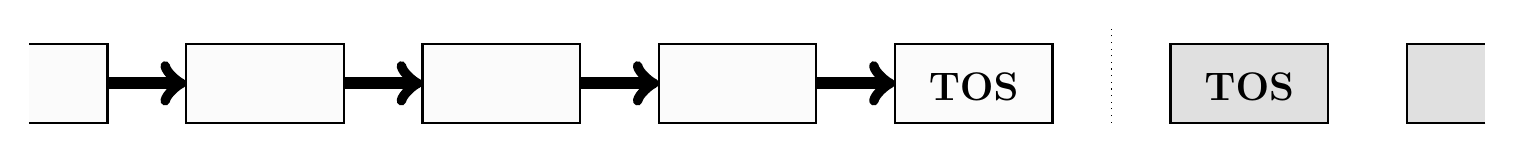
\begin{tikzpicture}
        \draw [thick, fill=gray!3]  (0,0) -- (1,0) -- (1,1) -- (0,1);%
        \draw [line width=1ex, ->]  (1,0.5) -- (2,0.5);              %
        \draw [thick, fill=gray!3]  (2,0) rectangle (4,1);           %PS+3
        \draw [line width=1ex, ->]  (4,0.5) -- (5,0.5);              %
        \draw [thick, fill=gray!3]  (5,0) rectangle (7,1);           %PS+2
        \draw [line width=1ex, ->]  (7,0.5) -- (8,0.5);              %
        \draw [thick, fill=gray!3]  (8,0) rectangle (10,1);          %PS+1
        \draw [line width=1ex, ->]  (10,0.5) -- (11,0.5);            %
        \draw [thick, fill=gray!3]  (11,0) rectangle (13,1);         %PS TOS
        \node at (12,0.45)          {\Large{\textbf{TOS}}};          %
        %\draw [line width=1ex, --] (13,0.5)  -- (14.5,0.5);         %
        \draw [dotted]              (13.75,0) -- (13.75,1.2);        %
        \draw [thick, fill=gray!24] (14.5,0) rectangle (16.5,1);     %RS TOS
        \node at (15.5,0.45)        {\Large{\textbf{TOS}}};          %
        %\draw [line width=1ex, --] (16.5,0.5) -- (17.5,0.5);        % 
        \draw [thick, fill=gray!24] (18.5,0) -- (17.5,0) -- (17.5,1) -- (18.5,1);
       \end{tikzpicture}
    }} &
    \texttt{0x06A8} \\ \hline   

    %DUP
    \texttt{DUP} &
    ( x -- x x ) &
    \multicolumn{1}{m{21.35em}|}{
    \scalebox{0.4} {
      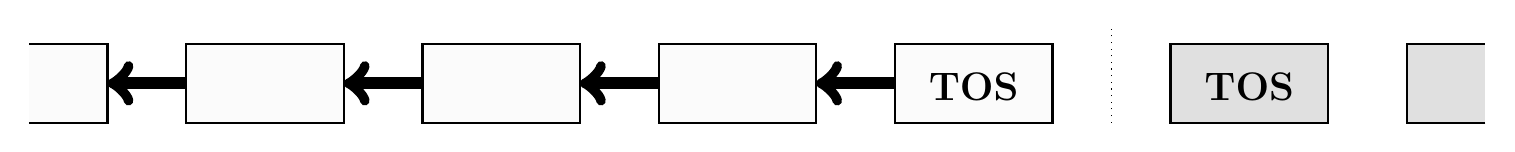
\begin{tikzpicture}
        \draw [thick, fill=gray!3]  (0,0) -- (1,0) -- (1,1) -- (0,1);%
        \draw [line width=1ex, <-]  (1,0.5) -- (2,0.5);              %
        \draw [thick, fill=gray!3]  (2,0) rectangle (4,1);           %PS+3
        \draw [line width=1ex, <-]  (4,0.5) -- (5,0.5);              %
        \draw [thick, fill=gray!3]  (5,0) rectangle (7,1);           %PS+2
        \draw [line width=1ex, <-]  (7,0.5) -- (8,0.5);              %
        \draw [thick, fill=gray!3]  (8,0) rectangle (10,1);          %PS+1
        \draw [line width=1ex, <-]  (10,0.5) -- (11,0.5);            %
        \draw [thick, fill=gray!3]  (11,0) rectangle (13,1);         %PS TOS
        \node at (12,0.45)          {\Large{\textbf{TOS}}};          %
        %\draw [line width=1ex, --] (13,0.5)  -- (14.5,0.5);         %
        \draw [dotted]              (13.75,0) -- (13.75,1.2);        %
        \draw [thick, fill=gray!24] (14.5,0) rectangle (16.5,1);     %RS TOS
        \node at (15.5,0.45)        {\Large{\textbf{TOS}}};          %
        %\draw [line width=1ex, --] (16.5,0.5) -- (17.5,0.5);        % 
        \draw [thick, fill=gray!24] (18.5,0) -- (17.5,0) -- (17.5,1) -- (18.5,1);
       \end{tikzpicture}
    }} &
    \texttt{0x0750} \\ \hline  

    %SWAP
    \texttt{SWAP} &
    ( x1 x2 -- x2 x1 ) &
    \multicolumn{1}{m{21.35em}|}{
    \scalebox{0.4} {
      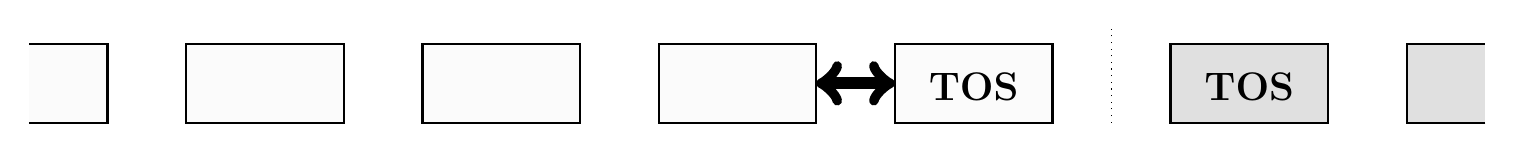
\begin{tikzpicture}
        \draw [thick, fill=gray!3]  (0,0) -- (1,0) -- (1,1) -- (0,1);%
        %\draw [line width=1ex, --] (1,0.5) -- (2,0.5);              %
        \draw [thick, fill=gray!3]  (2,0) rectangle (4,1);           %PS+3
        %\draw [line width=1ex, --] (4,0.5) -- (5,0.5);              %
        \draw [thick, fill=gray!3]  (5,0) rectangle (7,1);           %PS+2
        %\draw [line width=1ex, --] (7,0.5) -- (8,0.5);              %
        \draw [thick, fill=gray!3]  (8,0) rectangle (10,1);          %PS+1
        \draw [line width=1ex, <->] (10,0.5) -- (11,0.5);            %
        \draw [thick, fill=gray!3]  (11,0) rectangle (13,1);         %PS TOS
        \node at (12,0.45)          {\Large{\textbf{TOS}}};          %
        %\draw [line width=1ex, --] (13,0.5)  -- (14.5,0.5);         %
        \draw [dotted]              (13.75,0) -- (13.75,1.2);        %
        \draw [thick, fill=gray!24] (14.5,0) rectangle (16.5,1);     %RS TOS
        \node at (15.5,0.45)        {\Large{\textbf{TOS}}};          %
        %\draw [line width=1ex, --] (16.5,0.5) -- (17.5,0.5);        % 
        \draw [thick, fill=gray!24] (18.5,0) -- (17.5,0) -- (17.5,1) -- (18.5,1);
       \end{tikzpicture}
    }} &
    \texttt{0x0418} \\ \hline     

    %OVER
    \texttt{OVER} &
    ( x1 x2 -- x1 x2 x1 ) &
    \multicolumn{1}{m{21.35em}|}{
    \scalebox{0.4} {
      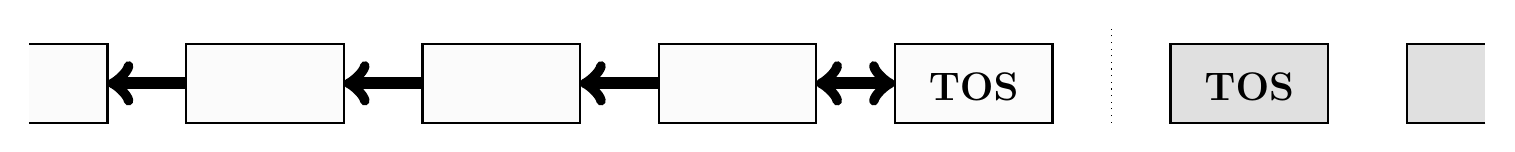
\begin{tikzpicture}
        \draw [thick, fill=gray!3]  (0,0) -- (1,0) -- (1,1) -- (0,1);%
        \draw [line width=1ex, <-]  (1,0.5) -- (2,0.5);              %
        \draw [thick, fill=gray!3]  (2,0) rectangle (4,1);           %PS+3
        \draw [line width=1ex, <-]  (4,0.5) -- (5,0.5);              %
        \draw [thick, fill=gray!3]  (5,0) rectangle (7,1);           %PS+2
        \draw [line width=1ex, <-]  (7,0.5) -- (8,0.5);              %
        \draw [thick, fill=gray!3]  (8,0) rectangle (10,1);          %PS+1
        \draw [line width=1ex, <->] (10,0.5) -- (11,0.5);            %
        \draw [thick, fill=gray!3]  (11,0) rectangle (13,1);         %PS TOS
        \node at (12,0.45)          {\Large{\textbf{TOS}}};          %
        %\draw [line width=1ex, --] (13,0.5)  -- (14.5,0.5);         %
        \draw [dotted]              (13.75,0) -- (13.75,1.2);        %
        \draw [thick, fill=gray!24] (14.5,0) rectangle (16.5,1);     %RS TOS
        \node at (15.5,0.45)        {\Large{\textbf{TOS}}};          %
        %\draw [line width=1ex, --] (16.5,0.5) -- (17.5,0.5);        % 
        \draw [thick, fill=gray!24] (18.5,0) -- (17.5,0) -- (17.5,1) -- (18.5,1);
       \end{tikzpicture}
    }} &
    \texttt{0x0758} \\ \hline     

    %NIP
    \texttt{NIP} &
    ( x1 x2 -- x2 ) &
    \multicolumn{1}{m{21.35em}|}{
    \scalebox{0.4} {
      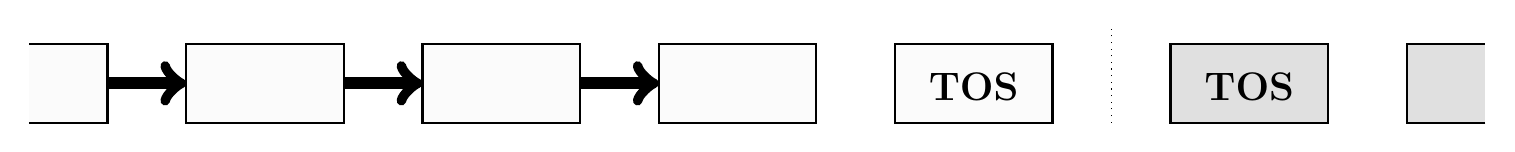
\begin{tikzpicture}
        \draw [thick, fill=gray!3]  (0,0) -- (1,0) -- (1,1) -- (0,1);%
        \draw [line width=1ex, ->]  (1,0.5) -- (2,0.5);              %
        \draw [thick, fill=gray!3]  (2,0) rectangle (4,1);           %PS+3
        \draw [line width=1ex, ->]  (4,0.5) -- (5,0.5);              %
        \draw [thick, fill=gray!3]  (5,0) rectangle (7,1);           %PS+2
        \draw [line width=1ex, ->]  (7,0.5) -- (8,0.5);              %
        \draw [thick, fill=gray!3]  (8,0) rectangle (10,1);          %PS+1
        %\draw [line width=1ex, ->] (10,0.5) -- (11,0.5);            %
        \draw [thick, fill=gray!3]  (11,0) rectangle (13,1);         %PS TOS
        \node at (12,0.45)          {\Large{\textbf{TOS}}};          %
        %\draw [line width=1ex, --] (13,0.5)  -- (14.5,0.5);         %
        \draw [dotted]              (13.75,0) -- (13.75,1.2);        %
        \draw [thick, fill=gray!24] (14.5,0) rectangle (16.5,1);     %RS TOS
        \node at (15.5,0.45)        {\Large{\textbf{TOS}}};          %
        %\draw [line width=1ex, --] (16.5,0.5) -- (17.5,0.5);        % 
        \draw [thick, fill=gray!24] (18.5,0) -- (17.5,0) -- (17.5,1) -- (18.5,1);
       \end{tikzpicture}
    }} &
    \texttt{0x06A0} \\ \hline  

    %TUCK
    \texttt{TUCK} &
    ( x1 x2 -- x2 x1 x2 ) &
    \multicolumn{1}{m{21.35em}|}{
    \scalebox{0.4} {
      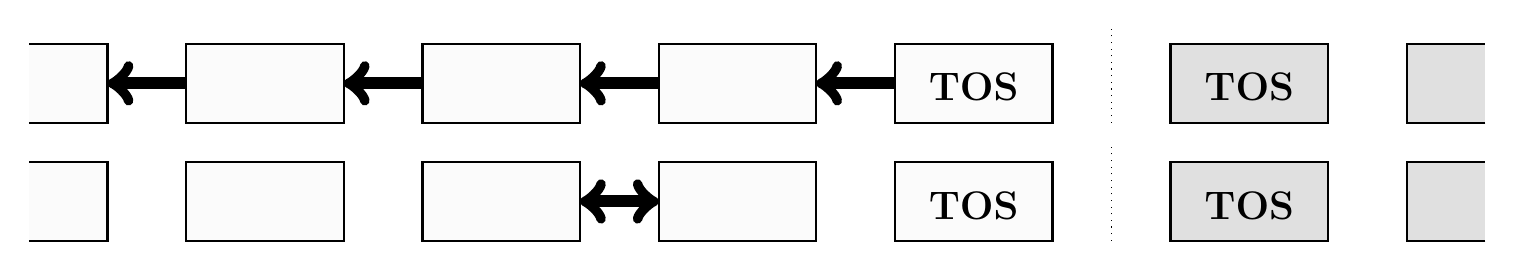
\begin{tikzpicture}
        \draw [thick, fill=gray!3]  (0,1.5) -- (1,1.5) -- (1,2.5) -- (0,2.5);%
        \draw [line width=1ex, <-]  (1,2)   -- (2,2);                %
        \draw [thick, fill=gray!3]  (2,1.5) rectangle (4,2.5);       %PS+3
        \draw [line width=1ex, <-]  (4,2)   -- (5,2);                %
        \draw [thick, fill=gray!3]  (5,1.5) rectangle (7,2.5);       %PS+2
        \draw [line width=1ex, <-]  (7,2)   -- (8,2);                %
        \draw [thick, fill=gray!3]  (8,1.5) rectangle (10,2.5);      %PS+1
        \draw [line width=1ex, <-]  (10,2)  -- (11,2);               %
        \draw [thick, fill=gray!3]  (11,1.5) rectangle (13,2.5);     %PS TOS
        \node at (12,1.95)          {\Large{\textbf{TOS}}};          %
        %\draw [line width=1ex, --] (13,2)  -- (14.5,2);             %
        \draw [dotted]              (13.75,1.5) -- (13.75,2.7);      %
        \draw [thick, fill=gray!24] (14.5,1.5) rectangle (16.5,2.5); %RS TOS
        \node at (15.5,1.95)        {\Large{\textbf{TOS}}};          %
        %\draw [line width=1ex, --] (16.5,2) -- (17.5,2);            % 
        \draw [thick, fill=gray!24] (18.5,1.5) -- (17.5,1.5) -- (17.5,2.5) -- (18.5,2.5);

        \draw [thick, fill=gray!3]  (0,0) -- (1,0) -- (1,1) -- (0,1);%
        %\draw [line width=1ex, --] (1,0.5) -- (2,0.5);              %
        \draw [thick, fill=gray!3]  (2,0) rectangle (4,1);           %PS+3
        %\draw [line width=1ex, --] (4,0.5) -- (5,0.5);              %
        \draw [thick, fill=gray!3]  (5,0) rectangle (7,1);           %PS+2
        \draw [line width=1ex, <->] (7,0.5) -- (8,0.5);              %
        \draw [thick, fill=gray!3]  (8,0) rectangle (10,1);          %PS+1
        %\draw [line width=1ex, --] (10,0.5) -- (11,0.5);            %
        \draw [thick, fill=gray!3]  (11,0) rectangle (13,1);         %PS TOS
        \node at (12,0.45)          {\Large{\textbf{TOS}}};          %
        %\draw [line width=1ex, --] (13,0.5)  -- (14.5,0.5);         %
        \draw [dotted]              (13.75,0) -- (13.75,1.2);        %
        \draw [thick, fill=gray!24] (14.5,0) rectangle (16.5,1);     %RS TOS
        \node at (15.5,0.45)        {\Large{\textbf{TOS}}};          %
        %\draw [line width=1ex, --] (16.5,0.5) -- (17.5,0.5);        % 
        \draw [thick, fill=gray!24] (18.5,0) -- (17.5,0) -- (17.5,1) -- (18.5,1);
       \end{tikzpicture}
    }} &
    \multicolumn{1}{m{4.25em}|}{
    \makecell[c]{ 
      \texttt{0x0750} \\ 
      \texttt{0x0460}
    }} \\ \hline

    %ROT
    \texttt{ROT} &
    ( x1 x2 x3 -- x2 x3 x1 ) &
    \multicolumn{1}{m{21.35em}|}{
    \scalebox{0.4} {
      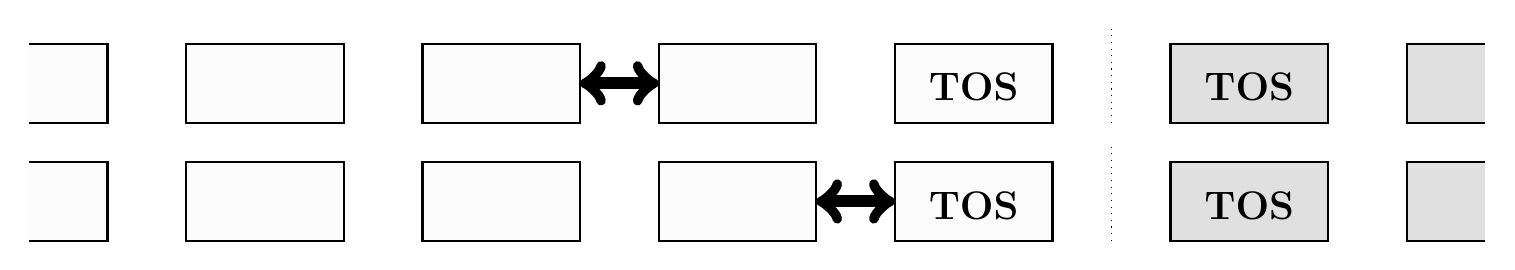
\begin{tikzpicture}
        \draw [thick, fill=gray!3]  (0,1.5) -- (1,1.5) -- (1,2.5) -- (0,2.5);%
        %\draw [line width=1ex, --] (1,2)   -- (2,2);                %
        \draw [thick, fill=gray!3]  (2,1.5) rectangle (4,2.5);       %PS+3
        %\draw [line width=1ex, --] (4,2)   -- (5,2);                %
        \draw [thick, fill=gray!3]  (5,1.5) rectangle (7,2.5);       %PS+2
        \draw [line width=1ex, <->] (7,2)   -- (8,2);                %
        \draw [thick, fill=gray!3]  (8,1.5) rectangle (10,2.5);      %PS+1
        %\draw [line width=1ex, --] (10,2) -- (11,2);                %
        \draw [thick, fill=gray!3]  (11,1.5) rectangle (13,2.5);     %PS TOS
        \node at (12,1.95)          {\Large{\textbf{TOS}}};          %
        %\draw [line width=1ex, --] (13,2)  -- (14.5,2);             %
        \draw [dotted]              (13.75,1.5) -- (13.75,2.7);      %
        \draw [thick, fill=gray!24] (14.5,1.5) rectangle (16.5,2.5); %RS TOS
        \node at (15.5,1.95)        {\Large{\textbf{TOS}}};          %
        %\draw [line width=1ex, --] (16.5,2) -- (17.5,2);            % 
        \draw [thick, fill=gray!24] (18.5,1.5) -- (17.5,1.5) -- (17.5,2.5) -- (18.5,2.5);

        \draw [thick, fill=gray!3]  (0,0) -- (1,0) -- (1,1) -- (0,1);%
        %\draw [line width=1ex, --] (1,0.5) -- (2,0.5);              %
        \draw [thick, fill=gray!3]  (2,0) rectangle (4,1);           %PS+3
        %\draw [line width=1ex, --] (4,0.5) -- (5,0.5);              %
        \draw [thick, fill=gray!3]  (5,0) rectangle (7,1);           %PS+2
        %\draw [line width=1ex, --] (7,0.5) -- (8,0.5);              %
        \draw [thick, fill=gray!3]  (8,0) rectangle (10,1);          %PS+1
        \draw [line width=1ex, <->] (10,0.5) -- (11,0.5);            %
        \draw [thick, fill=gray!3]  (11,0) rectangle (13,1);         %PS TOS
        \node at (12,0.45)          {\Large{\textbf{TOS}}};          %
        %\draw [line width=1ex, --] (13,0.5)  -- (14.5,0.5);         %
        \draw [dotted]              (13.75,0) -- (13.75,1.2);        %
        \draw [thick, fill=gray!24] (14.5,0) rectangle (16.5,1);     %RS TOS
        \node at (15.5,0.45)        {\Large{\textbf{TOS}}};          %
        %\draw [line width=1ex, --] (16.5,0.5) -- (17.5,0.5);        % 
        \draw [thick, fill=gray!24] (18.5,0) -- (17.5,0) -- (17.5,1) -- (18.5,1);
       \end{tikzpicture}
    }} &
    \multicolumn{1}{m{4.25em}|}{
    \makecell[c]{ 
      \texttt{0x0460} \\ 
      \texttt{0x0418}
    }} \\ \hline
    
    %-ROT
    \texttt{-ROT} &
    ( x1 x2 x3 -- x3 x1 x2 ) &
    \multicolumn{1}{m{21.35em}|}{
    \scalebox{0.4} {
      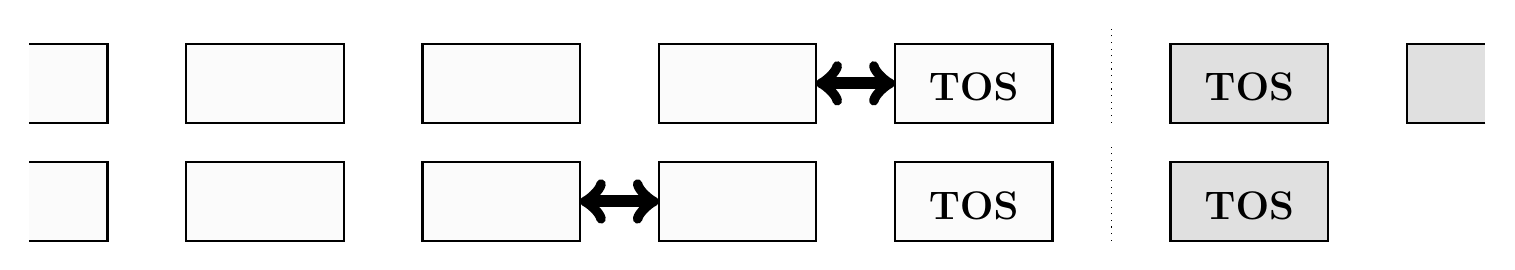
\begin{tikzpicture}
        \draw [thick, fill=gray!3]  (0,1.5) -- (1,1.5) -- (1,2.5) -- (0,2.5);%
        %\draw [line width=1ex, --] (1,2)   -- (2,2);                %
        \draw [thick, fill=gray!3]  (2,1.5) rectangle (4,2.5);       %PS+3
        %\draw [line width=1ex, --] (4,2)   -- (5,2);                %
        \draw [thick, fill=gray!3]  (5,1.5) rectangle (7,2.5);       %PS+2
        %\draw [line width=1ex, --] (7,2)   -- (8,2);                %
        \draw [thick, fill=gray!3]  (8,1.5) rectangle (10,2.5);      %PS+1
        \draw [line width=1ex, <->] (10,2) -- (11,2);                %
        \draw [thick, fill=gray!3]  (11,1.5) rectangle (13,2.5);     %PS TOS
        \node at (12,1.95)          {\Large{\textbf{TOS}}};          %
        %\draw [line width=1ex, --] (13,2)  -- (14.5,2);             %
        \draw [dotted]              (13.75,1.5) -- (13.75,2.7);      %
        \draw [thick, fill=gray!24] (14.5,1.5) rectangle (16.5,2.5); %RS TOS
        \node at (15.5,1.95)        {\Large{\textbf{TOS}}};          %
        %\draw [line width=1ex, --] (16.5,2) -- (17.5,2);            % 
        \draw [thick, fill=gray!24] (18.5,1.5) -- (17.5,1.5) -- (17.5,2.5) -- (18.5,2.5);

        \draw [thick, fill=gray!3]  (0,0) -- (1,0) -- (1,1) -- (0,1);%
        %\draw [line width=1ex, --] (1,0.5) -- (2,0.5);              %
        \draw [thick, fill=gray!3]  (2,0) rectangle (4,1);           %PS+3
        %\draw [line width=1ex, --] (4,0.5) -- (5,0.5);              %
        \draw [thick, fill=gray!3]  (5,0) rectangle (7,1);           %PS+2
        \draw [line width=1ex, <->] (7,0.5) -- (8,0.5);              %
        \draw [thick, fill=gray!3]  (8,0) rectangle (10,1);          %PS+1
        %\draw [line width=1ex, --] (10,0.5) -- (11,0.5);            %
        \draw [thick, fill=gray!3]  (11,0) rectangle (13,1);         %PS TOS
        \node at (12,0.45)          {\Large{\textbf{TOS}}};          %
        %\draw [line width=1ex, --] (13,0.5)  -- (14.5,0.5);         %
        \draw [dotted]              (13.75,0) -- (13.75,1.2);        %
        \draw [thick, fill=gray!24] (14.5,0) rectangle (16.5,1);     %RS TOS
        \node at (15.5,0.45)        {\Large{\textbf{TOS}}};          %
        %\draw [line width=1ex, --] (16.5,0.5) -- (17.5,0.5);        % 
      \end{tikzpicture}
    }} &
    \multicolumn{1}{m{4.25em}|}{
    \makecell[c]{ 
      \texttt{0x0418} \\ 
      \texttt{0x0460}
    }} \\ \hline

    %RDROP
    \texttt{RDROP} &
    ( R: x -- ) &
    \multicolumn{1}{m{21.35em}|}{
    \scalebox{0.4} {
      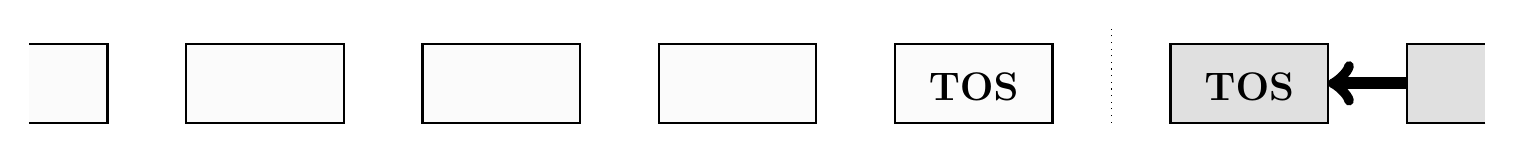
\begin{tikzpicture}
        \draw [thick, fill=gray!3]  (0,0) -- (1,0) -- (1,1) -- (0,1);%
        %\draw [line width=1ex, --] (1,0.5) -- (2,0.5);              %
        \draw [thick, fill=gray!3]  (2,0) rectangle (4,1);           %PS+3
        %\draw [line width=1ex, --] (4,0.5) -- (5,0.5);              %
        \draw [thick, fill=gray!3]  (5,0) rectangle (7,1);           %PS+2
        %\draw [line width=1ex, --] (7,0.5) -- (8,0.5);              %
        \draw [thick, fill=gray!3]  (8,0) rectangle (10,1);          %PS+1
        %\draw [line width=1ex, --] (10,0.5) -- (11,0.5);            %
        \draw [thick, fill=gray!3]  (11,0) rectangle (13,1);         %PS TOS
        \node at (12,0.45)          {\Large{\textbf{TOS}}};          %
        %\draw [line width=1ex, --] (13,0.5)  -- (14.5,0.5);         %
        \draw [dotted]              (13.75,0) -- (13.75,1.2);        %
        \draw [thick, fill=gray!24] (14.5,0) rectangle (16.5,1);     %RS TOS
        \node at (15.5,0.45)        {\Large{\textbf{TOS}}};          %
        \draw [line width=1ex, <-]  (16.5,0.5) -- (17.5,0.5);        % 
        \draw [thick, fill=gray!24] (18.5,0) -- (17.5,0) -- (17.5,1) -- (18.5,1);
       \end{tikzpicture}
    }} &
    \texttt{0x0401} \\ \hline     

    %RDUP
    \texttt{RDUP} &
    ( R: x -- x x ) &
    \multicolumn{1}{m{21.35em}|}{
    \scalebox{0.4} {
      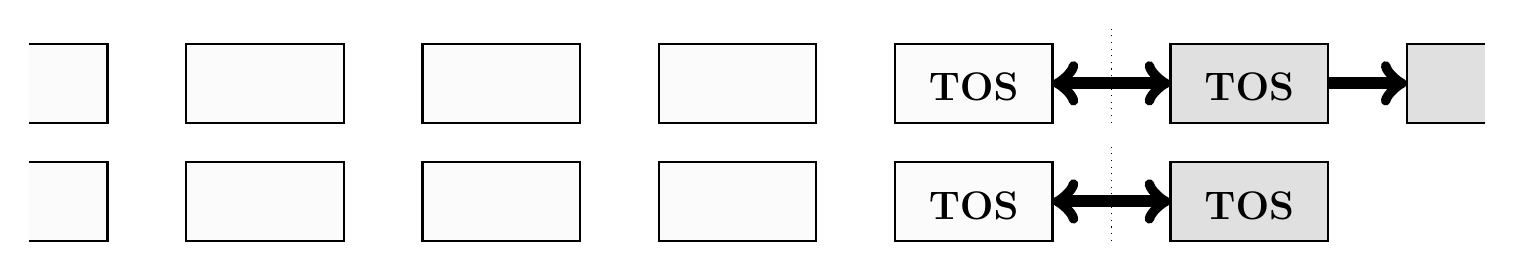
\begin{tikzpicture}
        \draw [thick, fill=gray!3]  (0,1.5) -- (1,1.5) -- (1,2.5) -- (0,2.5);%
        %\draw [line width=1ex, --] (1,2)   -- (2,2);                %
        \draw [thick, fill=gray!3]  (2,1.5) rectangle (4,2.5);       %PS+3
        %\draw [line width=1ex, --] (4,2)   -- (5,2);                %
        \draw [thick, fill=gray!3]  (5,1.5) rectangle (7,2.5);       %PS+2
        %\draw [line width=1ex, --] (7,2)   -- (8,2);                %
        \draw [thick, fill=gray!3]  (8,1.5) rectangle (10,2.5);      %PS+1
        %\draw [line width=1ex, --] (10,2) -- (11,2);                %
        \draw [thick, fill=gray!3]  (11,1.5) rectangle (13,2.5);     %PS TOS
        \node at (12,1.95)          {\Large{\textbf{TOS}}};          %
        \draw [line width=1ex, <->] (13,2)  -- (14.5,2);             %
        \draw [dotted]              (13.75,1.5) -- (13.75,2.7);      %
        \draw [thick, fill=gray!24] (14.5,1.5) rectangle (16.5,2.5); %RS TOS
        \node at (15.5,1.95)        {\Large{\textbf{TOS}}};          %
        \draw [line width=1ex, ->]  (16.5,2) -- (17.5,2);            % 
        \draw [thick, fill=gray!24] (18.5,1.5) -- (17.5,1.5) -- (17.5,2.5) -- (18.5,2.5);

        \draw [thick, fill=gray!3]  (0,0) -- (1,0) -- (1,1) -- (0,1);%
        %\draw [line width=1ex, --] (1,0.5) -- (2,0.5);              %
        \draw [thick, fill=gray!3]  (2,0) rectangle (4,1);           %PS+3
        %\draw [line width=1ex, --] (4,0.5) -- (5,0.5);              %
        \draw [thick, fill=gray!3]  (5,0) rectangle (7,1);           %PS+2
        %\draw [line width=1ex, --] (7,0.5) -- (8,0.5);              %
        \draw [thick, fill=gray!3]  (8,0) rectangle (10,1);          %PS+1
        %\draw [line width=1ex, --] (10,0.5) -- (11,0.5);            %
        \draw [thick, fill=gray!3]  (11,0) rectangle (13,1);         %PS TOS
        \node at (12,0.45)          {\Large{\textbf{TOS}}};          %
        \draw [line width=1ex, <->] (13,0.5)  -- (14.5,0.5);         %
        \draw [dotted]              (13.75,0) -- (13.75,1.2);        %
        \draw [thick, fill=gray!24] (14.5,0) rectangle (16.5,1);     %RS TOS
        \node at (15.5,0.45)        {\Large{\textbf{TOS}}};          %
        %\draw [line width=1ex, --] (16.5,0.5) -- (17.5,0.5);        % 
      \end{tikzpicture}
    }} &
    \multicolumn{1}{m{4.25em}|}{
    \makecell[c]{ 
      \texttt{0x0407} \\ 
      \texttt{0x0406}
    }} \\ \hline

    %>R
    \texttt{>R} &
    \multicolumn{1}{m{18.3em}|}{
    \makecell[c]{ 
      ( x -- )\\
      ( R: -- x )
    }} &
    \multicolumn{1}{m{21.35em}|}{
    \scalebox{0.4} {
      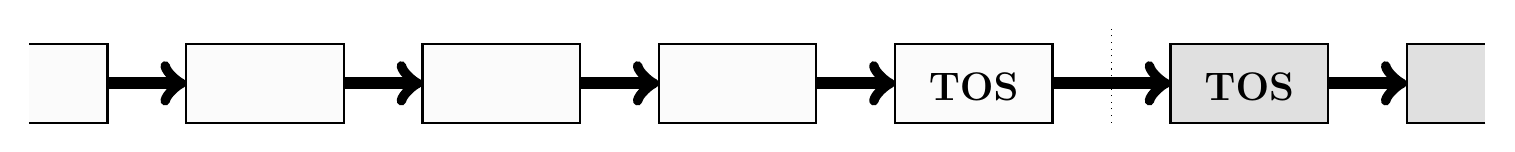
\begin{tikzpicture}
        \draw [thick, fill=gray!3]  (0,0) -- (1,0) -- (1,1) -- (0,1);%
        \draw [line width=1ex, ->]  (1,0.5) -- (2,0.5);              %
        \draw [thick, fill=gray!3]  (2,0) rectangle (4,1);           %PS+3
        \draw [line width=1ex, ->]  (4,0.5) -- (5,0.5);              %
        \draw [thick, fill=gray!3]  (5,0) rectangle (7,1);           %PS+2
        \draw [line width=1ex, ->]  (7,0.5) -- (8,0.5);              %
        \draw [thick, fill=gray!3]  (8,0) rectangle (10,1);          %PS+1
        \draw [line width=1ex, ->]  (10,0.5) -- (11,0.5);            %
        \draw [thick, fill=gray!3]  (11,0) rectangle (13,1);         %PS TOS
        \node at (12,0.45)          {\Large{\textbf{TOS}}};          %
        \draw [line width=1ex, ->]  (13,0.5)  -- (14.5,0.5);         %
        \draw [dotted]              (13.75,0) -- (13.75,1.2);        %
        \draw [thick, fill=gray!24] (14.5,0) rectangle (16.5,1);     %RS TOS
        \node at (15.5,0.45)        {\Large{\textbf{TOS}}};          %
        \draw [line width=1ex, ->]  (16.5,0.5) -- (17.5,0.5);        % 
        \draw [thick, fill=gray!24] (18.5,0) -- (17.5,0) -- (17.5,1) -- (18.5,1);
       \end{tikzpicture}
    }} &
    \texttt{0x06AB} \\ \hline  

    %R@
    \texttt{R@} &
    \multicolumn{1}{m{18.3em}|}{
    \makecell[c]{ 
      ( -- x )\\
      ( R: x -- x )
    }} &
    \multicolumn{1}{m{21.35em}|}{
    \scalebox{0.4} {
      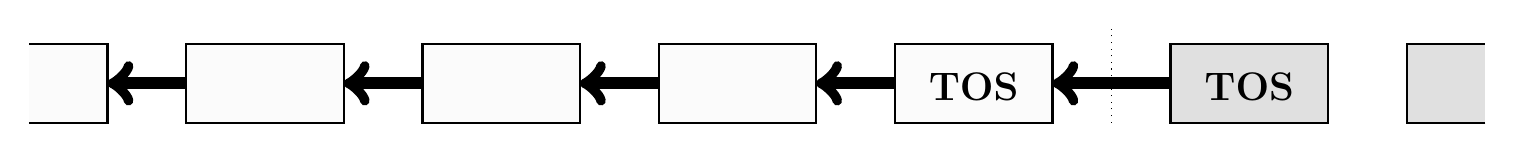
\begin{tikzpicture}
        \draw [thick, fill=gray!3]  (0,0) -- (1,0) -- (1,1) -- (0,1);%
        \draw [line width=1ex, <-]  (1,0.5) -- (2,0.5);              %
        \draw [thick, fill=gray!3]  (2,0) rectangle (4,1);           %PS+3
        \draw [line width=1ex, <-]  (4,0.5) -- (5,0.5);              %
        \draw [thick, fill=gray!3]  (5,0) rectangle (7,1);           %PS+2
        \draw [line width=1ex, <-]  (7,0.5) -- (8,0.5);              %
        \draw [thick, fill=gray!3]  (8,0) rectangle (10,1);          %PS+1
        \draw [line width=1ex, <-]  (10,0.5) -- (11,0.5);            %
        \draw [thick, fill=gray!3]  (11,0) rectangle (13,1);         %PS TOS
        \node at (12,0.45)          {\Large{\textbf{TOS}}};          %
        \draw [line width=1ex, <-]  (13,0.5)  -- (14.5,0.5);         %
        \draw [dotted]              (13.75,0) -- (13.75,1.2);        %
        \draw [thick, fill=gray!24] (14.5,0) rectangle (16.5,1);     %RS TOS
        \node at (15.5,0.45)        {\Large{\textbf{TOS}}};          %
        %\draw [line width=1ex, --] (16.5,0.5) -- (17.5,0.5);        % 
        \draw [thick, fill=gray!24] (18.5,0) -- (17.5,0) -- (17.5,1) -- (18.5,1);
       \end{tikzpicture}
    }} &
    \texttt{0x0754} \\ \hline  

    %R>
    \texttt{R>} &
    \multicolumn{1}{m{18.3em}|}{
    \makecell[c]{ 
      ( -- x )\\
      ( R: x -- )
    }} &
    \multicolumn{1}{m{21.35em}|}{
    \scalebox{0.4} {
      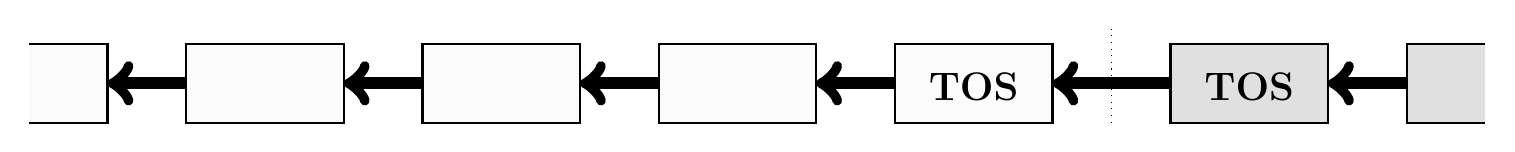
\begin{tikzpicture}
        \draw [thick, fill=gray!3]  (0,0) -- (1,0) -- (1,1) -- (0,1);%
        \draw [line width=1ex, <-]  (1,0.5) -- (2,0.5);              %
        \draw [thick, fill=gray!3]  (2,0) rectangle (4,1);           %PS+3
        \draw [line width=1ex, <-]  (4,0.5) -- (5,0.5);              %
        \draw [thick, fill=gray!3]  (5,0) rectangle (7,1);           %PS+2
        \draw [line width=1ex, <-]  (7,0.5) -- (8,0.5);              %
        \draw [thick, fill=gray!3]  (8,0) rectangle (10,1);          %PS+1
        \draw [line width=1ex, <-]  (10,0.5) -- (11,0.5);            %
        \draw [thick, fill=gray!3]  (11,0) rectangle (13,1);         %PS TOS
        \node at (12,0.45)          {\Large{\textbf{TOS}}};          %
        \draw [line width=1ex, <-]  (13,0.5)  -- (14.5,0.5);         %
        \draw [dotted]              (13.75,0) -- (13.75,1.2);        %
        \draw [thick, fill=gray!24] (14.5,0) rectangle (16.5,1);     %RS TOS
        \node at (15.5,0.45)        {\Large{\textbf{TOS}}};          %
        \draw [line width=1ex, <-]  (16.5,0.5) -- (17.5,0.5);        % 
        \draw [thick, fill=gray!24] (18.5,0) -- (17.5,0) -- (17.5,1) -- (18.5,1);
       \end{tikzpicture}
    }} &
    \texttt{0x0755} \\ \hline  

    %2DROP
    \texttt{2DROP} &
    ( x1 x2 -- ) &
    \multicolumn{1}{m{21.35em}|}{
    \scalebox{0.4} {
      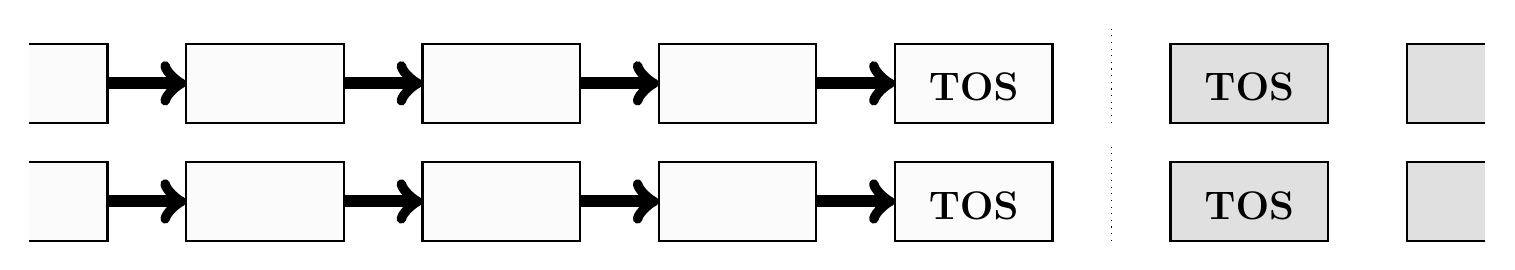
\begin{tikzpicture}
        \draw [thick, fill=gray!3]  (0,1.5) -- (1,1.5) -- (1,2.5) -- (0,2.5);%
        \draw [line width=1ex, ->]  (1,2)   -- (2,2);                %
        \draw [thick, fill=gray!3]  (2,1.5) rectangle (4,2.5);       %PS+3
        \draw [line width=1ex, ->]  (4,2)   -- (5,2);                %
        \draw [thick, fill=gray!3]  (5,1.5) rectangle (7,2.5);       %PS+2
        \draw [line width=1ex, ->]  (7,2)   -- (8,2);                %
        \draw [thick, fill=gray!3]  (8,1.5) rectangle (10,2.5);      %PS+1
        \draw [line width=1ex, ->]  (10,2)  -- (11,2);               %
        \draw [thick, fill=gray!3]  (11,1.5) rectangle (13,2.5);     %PS TOS
        \node at (12,1.95)          {\Large{\textbf{TOS}}};          %
        %\draw [line width=1ex, --] (13,2)  -- (14.5,2);             %
        \draw [dotted]              (13.75,1.5) -- (13.75,2.7);      %
        \draw [thick, fill=gray!24] (14.5,1.5) rectangle (16.5,2.5); %RS TOS
        \node at (15.5,1.95)        {\Large{\textbf{TOS}}};          %
        %\draw [line width=1ex, --] (16.5,2) -- (17.5,2);            % 
        \draw [thick, fill=gray!24] (18.5,1.5) -- (17.5,1.5) -- (17.5,2.5) -- (18.5,2.5);

        \draw [thick, fill=gray!3]  (0,0) -- (1,0) -- (1,1) -- (0,1);%
        \draw [line width=1ex, ->]  (1,0.5) -- (2,0.5);              %
        \draw [thick, fill=gray!3]  (2,0) rectangle (4,1);           %PS+3
        \draw [line width=1ex, ->]  (4,0.5) -- (5,0.5);              %
        \draw [thick, fill=gray!3]  (5,0) rectangle (7,1);           %PS+2
        \draw [line width=1ex, ->]  (7,0.5) -- (8,0.5);              %
        \draw [thick, fill=gray!3]  (8,0) rectangle (10,1);          %PS+1
        \draw [line width=1ex, ->]  (10,0.5) -- (11,0.5);            %
        \draw [thick, fill=gray!3]  (11,0) rectangle (13,1);         %PS TOS
        \node at (12,0.45)          {\Large{\textbf{TOS}}};          %
        %\draw [line width=1ex, --] (13,0.5)  -- (14.5,0.5);         %
        \draw [dotted]              (13.75,0) -- (13.75,1.2);        %
        \draw [thick, fill=gray!24] (14.5,0) rectangle (16.5,1);     %RS TOS
        \node at (15.5,0.45)        {\Large{\textbf{TOS}}};          %
        %\draw [line width=1ex, --] (16.5,0.5) -- (17.5,0.5);        % 
        \draw [thick, fill=gray!24] (18.5,0) -- (17.5,0) -- (17.5,1) -- (18.5,1);
      \end{tikzpicture}
    }} &
    \multicolumn{1}{m{4.25em}|}{
    \makecell[c]{ 
      \texttt{0x06A8} \\ 
      \texttt{0x06A8}
    }} \\ \hline

    %2DUP
    \texttt{2DUP} &
    ( x1 x2 -- x1 x2 x1 x2 ) &
    \multicolumn{1}{m{21.35em}|}{
    \scalebox{0.4} {
      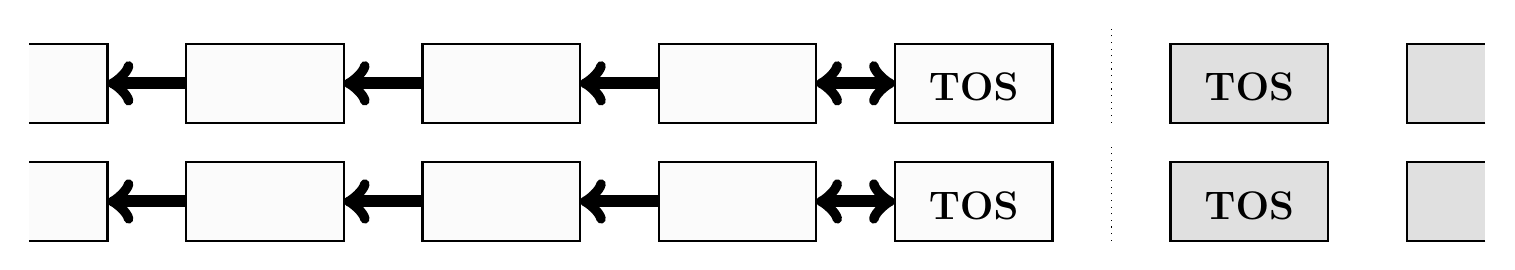
\begin{tikzpicture}
        \draw [thick, fill=gray!3]  (0,1.5) -- (1,1.5) -- (1,2.5) -- (0,2.5);%
        \draw [line width=1ex, <-]  (1,2)   -- (2,2);                %
        \draw [thick, fill=gray!3]  (2,1.5) rectangle (4,2.5);       %PS+3
        \draw [line width=1ex, <-]  (4,2)   -- (5,2);                %
        \draw [thick, fill=gray!3]  (5,1.5) rectangle (7,2.5);       %PS+2
        \draw [line width=1ex, <-]  (7,2)   -- (8,2);                %
        \draw [thick, fill=gray!3]  (8,1.5) rectangle (10,2.5);      %PS+1
        \draw [line width=1ex, <->] (10,2)  -- (11,2);               %
        \draw [thick, fill=gray!3]  (11,1.5) rectangle (13,2.5);     %PS TOS
        \node at (12,1.95)          {\Large{\textbf{TOS}}};          %
        %\draw [line width=1ex, --] (13,2)  -- (14.5,2);             %
        \draw [dotted]              (13.75,1.5) -- (13.75,2.7);      %
        \draw [thick, fill=gray!24] (14.5,1.5) rectangle (16.5,2.5); %RS TOS
        \node at (15.5,1.95)        {\Large{\textbf{TOS}}};          %
        %\draw [line width=1ex, --] (16.5,2) -- (17.5,2);            % 
        \draw [thick, fill=gray!24] (18.5,1.5) -- (17.5,1.5) -- (17.5,2.5) -- (18.5,2.5);

        \draw [thick, fill=gray!3]  (0,0) -- (1,0) -- (1,1) -- (0,1);%
        \draw [line width=1ex, <-]  (1,0.5) -- (2,0.5);              %
        \draw [thick, fill=gray!3]  (2,0) rectangle (4,1);           %PS+3
        \draw [line width=1ex, <-]  (4,0.5) -- (5,0.5);              %
        \draw [thick, fill=gray!3]  (5,0) rectangle (7,1);           %PS+2
        \draw [line width=1ex, <-]  (7,0.5) -- (8,0.5);              %
        \draw [thick, fill=gray!3]  (8,0) rectangle (10,1);          %PS+1
        \draw [line width=1ex, <->] (10,0.5) -- (11,0.5);            %
        \draw [thick, fill=gray!3]  (11,0) rectangle (13,1);         %PS TOS
        \node at (12,0.45)          {\Large{\textbf{TOS}}};          %
        %\draw [line width=1ex, --] (13,0.5)  -- (14.5,0.5);         %
        \draw [dotted]              (13.75,0) -- (13.75,1.2);        %
        \draw [thick, fill=gray!24] (14.5,0) rectangle (16.5,1);     %RS TOS
        \node at (15.5,0.45)        {\Large{\textbf{TOS}}};          %
        %\draw [line width=1ex, --] (16.5,0.5) -- (17.5,0.5);        % 
        \draw [thick, fill=gray!24] (18.5,0) -- (17.5,0) -- (17.5,1) -- (18.5,1);
      \end{tikzpicture}
    }} &
    \multicolumn{1}{m{4.25em}|}{
    \makecell[c]{ 
      \texttt{0x0758} \\
      \texttt{0x0758}
    }} \\ \hline

    %2SWAP
    \texttt{2SWAP} &
    ( x1 x2 x3 x4 -- x3 x4 x1 x2 ) &
    \multicolumn{1}{m{21.35em}|}{
    \scalebox{0.4} {
      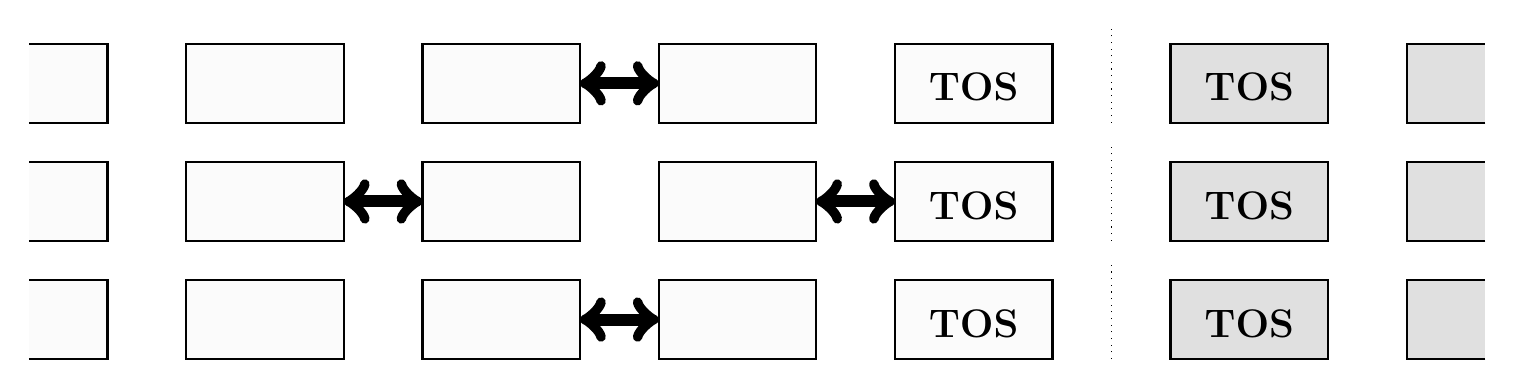
\begin{tikzpicture}
        \draw [thick, fill=gray!3]  (0,3) -- (1,3) -- (1,4) -- (0,4);%
        %\draw [line width=1ex, --] (1,3.5)   -- (2,3.5);            %
        \draw [thick, fill=gray!3]  (2,3) rectangle (4,4);           %PS+3
        %\draw [line width=1ex, --] (4,3.5)   -- (5,3.5);            %
        \draw [thick, fill=gray!3]  (5,3) rectangle (7,4);           %PS+2
        \draw [line width=1ex, <->] (7,3.5)   -- (8,3.5);            %
        \draw [thick, fill=gray!3]  (8,3) rectangle (10,4);          %PS+1
        %\draw [line width=1ex, --] (10,3.5)  -- (11,3.5);           %
        \draw [thick, fill=gray!3]  (11,3) rectangle (13,4);         %PS TOS
        \node at (12,3.45)          {\Large{\textbf{TOS}}};          %
        %\draw [line width=1ex, --] (13,3.5)  -- (14.5,3.5);         %
        \draw [dotted]              (13.75,3) -- (13.75,4.2);        %
        \draw [thick, fill=gray!24] (14.5,3) rectangle (16.5,4);     %RS TOS
        \node at (15.5,3.45)        {\Large{\textbf{TOS}}};          %
        %\draw [line width=1ex, --] (16.5,3.5) -- (17.5,3.5);        % 
        \draw [thick, fill=gray!24] (18.5,3)   -- (17.5,3) -- (17.5,4) -- (18.5,4);

        \draw [thick, fill=gray!3]  (0,1.5) -- (1,1.5) -- (1,2.5) -- (0,2.5);%
        %\draw [line width=1ex, --] (1,2)   -- (2,2);                %
        \draw [thick, fill=gray!3]  (2,1.5) rectangle (4,2.5);       %PS+3
        \draw [line width=1ex, <->] (4,2)   -- (5,2);                %
        \draw [thick, fill=gray!3]  (5,1.5) rectangle (7,2.5);       %PS+2
        %\draw [line width=1ex, --] (7,2)   -- (8,2);                %
        \draw [thick, fill=gray!3]  (8,1.5) rectangle (10,2.5);      %PS+1
        \draw [line width=1ex, <->] (10,2)  -- (11,2);               %
        \draw [thick, fill=gray!3]  (11,1.5) rectangle (13,2.5);     %PS TOS
        \node at (12,1.95)          {\Large{\textbf{TOS}}};          %
        %\draw [line width=1ex, --] (13,2)  -- (14.5,2);             %
        \draw [dotted]              (13.75,1.5) -- (13.75,2.7);      %
        \draw [thick, fill=gray!24] (14.5,1.5) rectangle (16.5,2.5); %RS TOS
        \node at (15.5,1.95)        {\Large{\textbf{TOS}}};          %
        %\draw [line width=1ex, --] (16.5,2) -- (17.5,2);            % 
        \draw [thick, fill=gray!24] (18.5,1.5) -- (17.5,1.5) -- (17.5,2.5) -- (18.5,2.5);

        \draw [thick, fill=gray!3]  (0,0) -- (1,0) -- (1,1) -- (0,1);%
        %\draw [line width=1ex, --] (1,0.5) -- (2,0.5);              %
        \draw [thick, fill=gray!3]  (2,0) rectangle (4,1);           %PS+3
        %\draw [line width=1ex, --] (4,0.5) -- (5,0.5);              %
        \draw [thick, fill=gray!3]  (5,0) rectangle (7,1);           %PS+2
        \draw [line width=1ex, <->] (7,0.5) -- (8,0.5);              %
        \draw [thick, fill=gray!3]  (8,0) rectangle (10,1);          %PS+1
        %\draw [line width=1ex, --] (10,0.5) -- (11,0.5);            %
        \draw [thick, fill=gray!3]  (11,0) rectangle (13,1);         %PS TOS
        \node at (12,0.45)          {\Large{\textbf{TOS}}};          %
        %\draw [line width=1ex, --] (13,0.5)  -- (14.5,0.5);         %
        \draw [dotted]              (13.75,0) -- (13.75,1.2);        %
        \draw [thick, fill=gray!24] (14.5,0) rectangle (16.5,1);     %RS TOS
        \node at (15.5,0.45)        {\Large{\textbf{TOS}}};          %
        %\draw [line width=1ex, --] (16.5,0.5) -- (17.5,0.5);        % 
        \draw [thick, fill=gray!24] (18.5,0) -- (17.5,0) -- (17.5,1) -- (18.5,1);
      \end{tikzpicture}
    }} &
    \multicolumn{1}{m{4.25em}|}{
    \makecell[c]{ 
      \texttt{0x0460} \\ 
      \texttt{0x0598} \\ 
      \texttt{0x0460}
    }} \\ \hline

    %2OVER
    \texttt{2OVER} &
    ( x1 x2 x3 x4 -- x1 x2 x3 x4 x1 x2 ) &
    \multicolumn{1}{m{21.35em}|}{
    \scalebox{0.4} {
      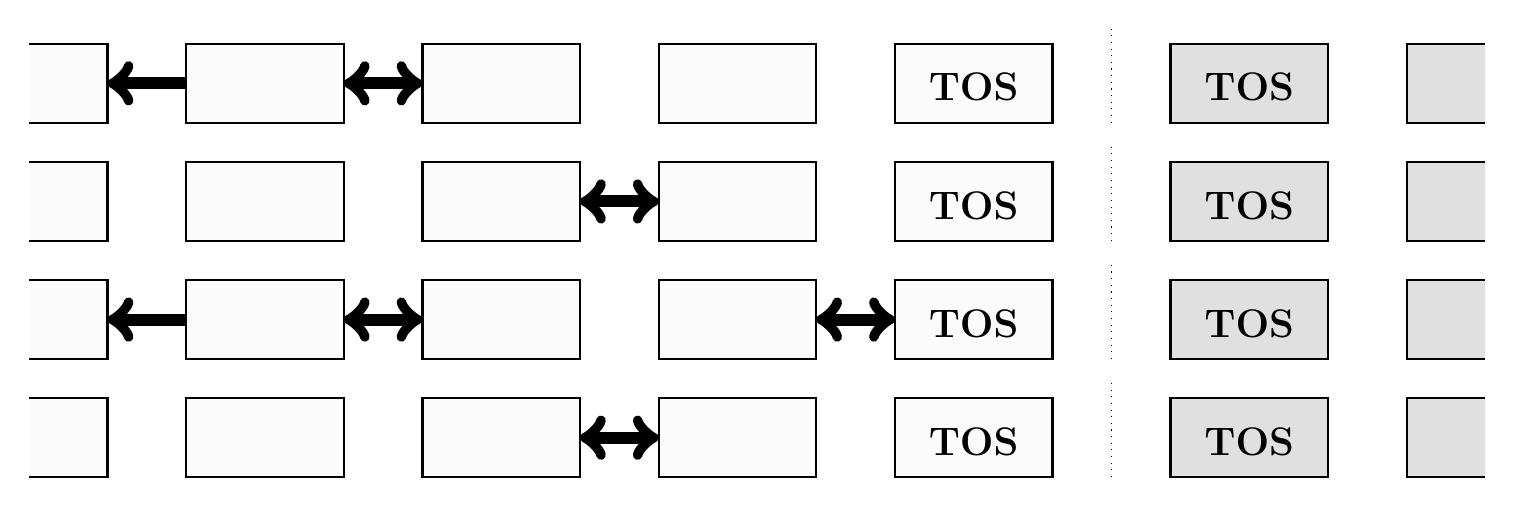
\begin{tikzpicture}
        \draw [thick, fill=gray!3]  (0,4.5) -- (1,4.5) -- (1,5.5) -- (0,5.5);%
        \draw [line width=1ex, <-]  (1,5)   -- (2,5);                %
        \draw [thick, fill=gray!3]  (2,4.5) rectangle (4,5.5);       %PS+3
        \draw [line width=1ex, <->] (4,5)   -- (5,5);                %
        \draw [thick, fill=gray!3]  (5,4.5) rectangle (7,5.5);       %PS+2
        %\draw [line width=1ex, --] (7,5)   -- (8,5);                %
        \draw [thick, fill=gray!3]  (8,4.5) rectangle (10,5.5);      %PS+1
        %\draw [line width=1ex, --] (10,5)  -- (11,5);               %
        \draw [thick, fill=gray!3]  (11,4.5) rectangle (13,5.5);     %PS TOS
        \node at (12,4.95)          {\Large{\textbf{TOS}}};          %
        %\draw [line width=1ex, --] (13,5)  -- (14.5,5);             %
        \draw [dotted]              (13.75,4.5) -- (13.75,5.7);      %
        \draw [thick, fill=gray!24] (14.5,4.5) rectangle (16.5,5.5); %RS TOS
        \node at (15.5,4.95)        {\Large{\textbf{TOS}}};          %
        %\draw [line width=1ex, --] (16.5,5) -- (17.5,5);            % 
        \draw [thick, fill=gray!24] (18.5,4.5) -- (17.5,4.5) -- (17.5,5.5) -- (18.5,5.5);

        \draw [thick, fill=gray!3]  (0,3) -- (1,3) -- (1,4) -- (0,4);%
        %\draw [line width=1ex, --] (1,3.5)   -- (2,3.5);            %
        \draw [thick, fill=gray!3]  (2,3) rectangle (4,4);           %PS+3
        %\draw [line width=1ex, --] (4,3.5)   -- (5,3.5);            %
        \draw [thick, fill=gray!3]  (5,3) rectangle (7,4);           %PS+2
        \draw [line width=1ex, <->] (7,3.5)   -- (8,3.5);            %
        \draw [thick, fill=gray!3]  (8,3) rectangle (10,4);          %PS+1
        %\draw [line width=1ex, --] (10,3.5)  -- (11,3.5);           %
        \draw [thick, fill=gray!3]  (11,3) rectangle (13,4);         %PS TOS
        \node at (12,3.45)          {\Large{\textbf{TOS}}};          %
        %\draw [line width=1ex, --] (13,3.5)  -- (14.5,3.5);         %
        \draw [dotted]              (13.75,3) -- (13.75,4.2);        %
        \draw [thick, fill=gray!24] (14.5,3) rectangle (16.5,4);     %RS TOS
        \node at (15.5,3.45)        {\Large{\textbf{TOS}}};          %
        %\draw [line width=1ex, --] (16.5,3.5) -- (17.5,3.5);        % 
        \draw [thick, fill=gray!24] (18.5,3)   -- (17.5,3) -- (17.5,4) -- (18.5,4);

        \draw [thick, fill=gray!3]  (0,1.5) -- (1,1.5) -- (1,2.5) -- (0,2.5);%
        \draw [line width=1ex, <-]  (1,2)   -- (2,2);                %
        \draw [thick, fill=gray!3]  (2,1.5) rectangle (4,2.5);       %PS+3
        \draw [line width=1ex, <->] (4,2)   -- (5,2);                %
        \draw [thick, fill=gray!3]  (5,1.5) rectangle (7,2.5);       %PS+2
        %\draw [line width=1ex, --] (7,2)   -- (8,2);                %
        \draw [thick, fill=gray!3]  (8,1.5) rectangle (10,2.5);      %PS+1
        \draw [line width=1ex, <->] (10,2)  -- (11,2);               %
        \draw [thick, fill=gray!3]  (11,1.5) rectangle (13,2.5);     %PS TOS
        \node at (12,1.95)          {\Large{\textbf{TOS}}};          %
        %\draw [line width=1ex, --] (13,2)  -- (14.5,2);             %
        \draw [dotted]              (13.75,1.5) -- (13.75,2.7);      %
        \draw [thick, fill=gray!24] (14.5,1.5) rectangle (16.5,2.5); %RS TOS
        \node at (15.5,1.95)        {\Large{\textbf{TOS}}};          %
        %\draw [line width=1ex, --] (16.5,2) -- (17.5,2);            % 
        \draw [thick, fill=gray!24] (18.5,1.5) -- (17.5,1.5) -- (17.5,2.5) -- (18.5,2.5);

        \draw [thick, fill=gray!3]  (0,0) -- (1,0) -- (1,1) -- (0,1);%
        %\draw [line width=1ex, --] (1,0.5) -- (2,0.5);              %
        \draw [thick, fill=gray!3]  (2,0) rectangle (4,1);           %PS+3
        %\draw [line width=1ex, --] (4,0.5) -- (5,0.5);              %
        \draw [thick, fill=gray!3]  (5,0) rectangle (7,1);           %PS+2
        \draw [line width=1ex, <->] (7,0.5) -- (8,0.5);              %
        \draw [thick, fill=gray!3]  (8,0) rectangle (10,1);          %PS+1
        %\draw [line width=1ex, --] (10,0.5) -- (11,0.5);            %
        \draw [thick, fill=gray!3]  (11,0) rectangle (13,1);         %PS TOS
        \node at (12,0.45)          {\Large{\textbf{TOS}}};          %
        %\draw [line width=1ex, --] (13,0.5)  -- (14.5,0.5);         %
        \draw [dotted]              (13.75,0) -- (13.75,1.2);        %
        \draw [thick, fill=gray!24] (14.5,0) rectangle (16.5,1);     %RS TOS
        \node at (15.5,0.45)        {\Large{\textbf{TOS}}};          %
        %\draw [line width=1ex, --] (16.5,0.5) -- (17.5,0.5);        % 
        \draw [thick, fill=gray!24] (18.5,0) -- (17.5,0) -- (17.5,1) -- (18.5,1);
      \end{tikzpicture}
    }} &
    \multicolumn{1}{m{4.25em}|}{
    \makecell[c]{ 
      \texttt{0x0780} \\ 
      \texttt{0x0460} \\ 
      \texttt{0x0798} \\ 
      \texttt{0x0460}
    }} \\ \hline

    %2NIP
    \texttt{2NIP} &
    ( x1 x2 x3 x4 -- x3 x4 ) &
    \multicolumn{1}{m{21.35em}|}{
    \scalebox{0.4} {
      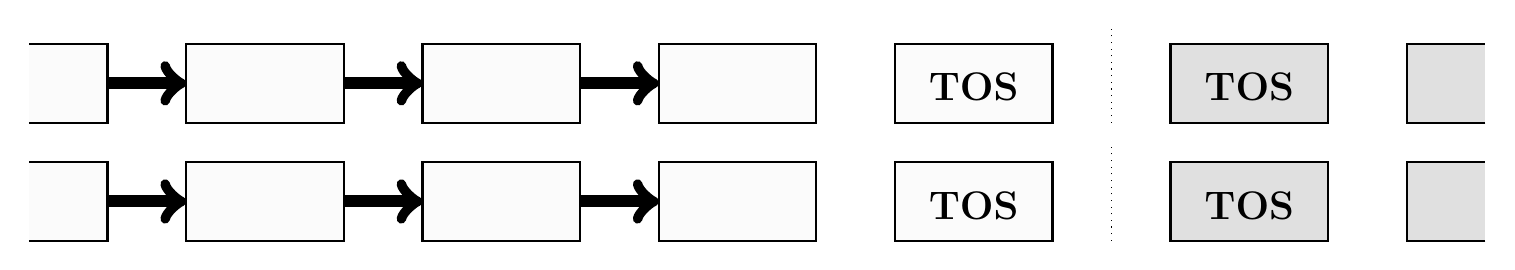
\begin{tikzpicture}
        \draw [thick, fill=gray!3]  (0,1.5) -- (1,1.5) -- (1,2.5) -- (0,2.5);%
        \draw [line width=1ex, ->]  (1,2)   -- (2,2);                %
        \draw [thick, fill=gray!3]  (2,1.5) rectangle (4,2.5);       %PS+3
        \draw [line width=1ex, ->]  (4,2)   -- (5,2);                %
        \draw [thick, fill=gray!3]  (5,1.5) rectangle (7,2.5);       %PS+2
        \draw [line width=1ex, ->]  (7,2)   -- (8,2);                %
        \draw [thick, fill=gray!3]  (8,1.5) rectangle (10,2.5);      %PS+1
        %\draw [line width=1ex, --] (10,2)  -- (11,2);               %
        \draw [thick, fill=gray!3]  (11,1.5) rectangle (13,2.5);     %PS TOS
        \node at (12,1.95)          {\Large{\textbf{TOS}}};          %
        %\draw [line width=1ex, --] (13,2)  -- (14.5,2);             %
        \draw [dotted]              (13.75,1.5) -- (13.75,2.7);      %
        \draw [thick, fill=gray!24] (14.5,1.5) rectangle (16.5,2.5); %RS TOS
        \node at (15.5,1.95)        {\Large{\textbf{TOS}}};          %
        %\draw [line width=1ex, --] (16.5,2) -- (17.5,2);            % 
        \draw [thick, fill=gray!24] (18.5,1.5) -- (17.5,1.5) -- (17.5,2.5) -- (18.5,2.5);

        \draw [thick, fill=gray!3]  (0,0) -- (1,0) -- (1,1) -- (0,1);%
        \draw [line width=1ex, ->]  (1,0.5) -- (2,0.5);              %
        \draw [thick, fill=gray!3]  (2,0) rectangle (4,1);           %PS+3
        \draw [line width=1ex, ->]  (4,0.5) -- (5,0.5);              %
        \draw [thick, fill=gray!3]  (5,0) rectangle (7,1);           %PS+2
        \draw [line width=1ex, ->]  (7,0.5) -- (8,0.5);              %
        \draw [thick, fill=gray!3]  (8,0) rectangle (10,1);          %PS+1
        %\draw [line width=1ex, --] (10,0.5) -- (11,0.5);            %
        \draw [thick, fill=gray!3]  (11,0) rectangle (13,1);         %PS TOS
        \node at (12,0.45)          {\Large{\textbf{TOS}}};          %
        %\draw [line width=1ex, --] (13,0.5)  -- (14.5,0.5);         %
        \draw [dotted]              (13.75,0) -- (13.75,1.2);        %
        \draw [thick, fill=gray!24] (14.5,0) rectangle (16.5,1);     %RS TOS
        \node at (15.5,0.45)        {\Large{\textbf{TOS}}};          %
        %\draw [line width=1ex, --] (16.5,0.5) -- (17.5,0.5);        % 
        \draw [thick, fill=gray!24] (18.5,0) -- (17.5,0) -- (17.5,1) -- (18.5,1);
      \end{tikzpicture}
    }} &
    \multicolumn{1}{m{4.25em}|}{
    \makecell[c]{ 
      \texttt{0x06A0} \\ 
      \texttt{0x06A0}
    }} \\ \hline

    %2TUCK
    \texttt{2TUCK} &
    ( x1 x2 x3 x4 -- x3 x4 x1 x2 x3 x4 ) &
    \multicolumn{1}{m{21.35em}|}{
    \scalebox{0.4} {
      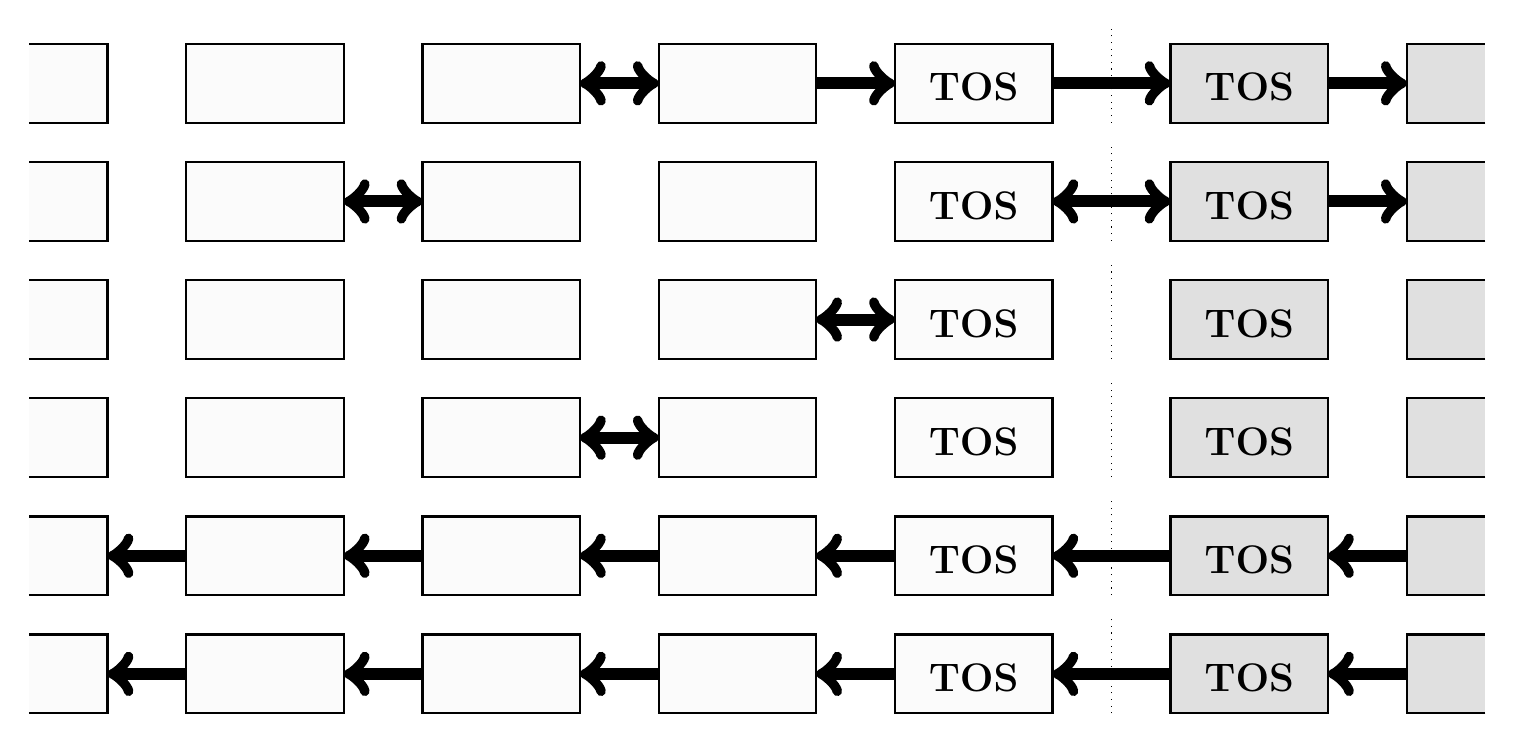
\begin{tikzpicture}
        \draw [thick, fill=gray!3]  (0,7.5) -- (1,7.5) -- (1,8.5) -- (0,8.5);%
        %\draw [line width=1ex, --] (1,8)   -- (2,8);                %
        \draw [thick, fill=gray!3]  (2,7.5) rectangle (4,8.5);       %PS+3
        %\draw [line width=1ex, --] (4,8)   -- (5,8);                %
        \draw [thick, fill=gray!3]  (5,7.5) rectangle (7,8.5);       %PS+2
        \draw [line width=1ex, <->] (7,8)   -- (8,8);                %
        \draw [thick, fill=gray!3]  (8,7.5) rectangle (10,8.5);      %PS+1
        \draw [line width=1ex, ->]  (10,8)  -- (11,8);               %
        \draw [thick, fill=gray!3]  (11,7.5) rectangle (13,8.5);     %PS TOS
        \node at (12,7.95)          {\Large{\textbf{TOS}}};          %
        \draw [line width=1ex, ->]  (13,8)  -- (14.5,8);             %
        \draw [dotted]              (13.75,7.5) -- (13.75,8.7);      %
        \draw [thick, fill=gray!24] (14.5,7.5) rectangle (16.5,8.5); %RS TOS
        \node at (15.5,7.95)        {\Large{\textbf{TOS}}};          %
        \draw [line width=1ex, ->]  (16.5,8) -- (17.5,8);            % 
        \draw [thick, fill=gray!24] (18.5,7.5) -- (17.5,7.5) -- (17.5,8.5) -- (18.5,8.5);

        \draw [thick, fill=gray!3]  (0,6) -- (1,6) -- (1,7) -- (0,7);%
        %\draw [line width=1ex, --] (1,6.5)   -- (2,6.5);            %
        \draw [thick, fill=gray!3]  (2,6) rectangle (4,7);           %PS+3
        \draw [line width=1ex, <->] (4,6.5)   -- (5,6.5);            %
        \draw [thick, fill=gray!3]  (5,6) rectangle (7,7);           %PS+2
        %\draw [line width=1ex, --] (7,6.5)   -- (8,6.5);            %
        \draw [thick, fill=gray!3]  (8,6) rectangle (10,7);          %PS+1
        %\draw [line width=1ex, --] (10,6.5)  -- (11,6.5);           %
        \draw [thick, fill=gray!3]  (11,6) rectangle (13,7);         %PS TOS
        \node at (12,6.45)          {\Large{\textbf{TOS}}};          %
        \draw [line width=1ex, <->] (13,6.5)  -- (14.5,6.5);         %
        \draw [dotted]              (13.75,6) -- (13.75,7.2);        %
        \draw [thick, fill=gray!24] (14.5,6) rectangle (16.5,7);     %RS TOS
        \node at (15.5,6.45)        {\Large{\textbf{TOS}}};          %
        \draw [line width=1ex, ->]  (16.5,6.5) -- (17.5,6.5);         % 
        \draw [thick, fill=gray!24] (18.5,6)   -- (17.5,6) -- (17.5,7) -- (18.5,7);

        \draw [thick, fill=gray!3]  (0,4.5) -- (1,4.5) -- (1,5.5) -- (0,5.5);%
        %\draw [line width=1ex, --] (1,5)   -- (2,5);                %
        \draw [thick, fill=gray!3]  (2,4.5) rectangle (4,5.5);       %PS+3
        %\draw [line width=1ex, --] (4,5)   -- (5,5);                %
        \draw [thick, fill=gray!3]  (5,4.5) rectangle (7,5.5);       %PS+2
        %\draw [line width=1ex, --] (7,5)   -- (8,5);                %
        \draw [thick, fill=gray!3]  (8,4.5) rectangle (10,5.5);      %PS+1
        \draw [line width=1ex, <->] (10,5)  -- (11,5);               %
        \draw [thick, fill=gray!3]  (11,4.5) rectangle (13,5.5);     %PS TOS
        \node at (12,4.95)          {\Large{\textbf{TOS}}};          %
        %\draw [line width=1ex, --] (13,5)  -- (14.5,5);             %
        \draw [dotted]              (13.75,4.5) -- (13.75,5.7);      %
        \draw [thick, fill=gray!24] (14.5,4.5) rectangle (16.5,5.5); %RS TOS
        \node at (15.5,4.95)        {\Large{\textbf{TOS}}};          %
        %\draw [line width=1ex, --] (16.5,5) -- (17.5,5);            % 
        \draw [thick, fill=gray!24] (18.5,4.5) -- (17.5,4.5) -- (17.5,5.5) -- (18.5,5.5);

        \draw [thick, fill=gray!3]  (0,3) -- (1,3) -- (1,4) -- (0,4);%
        %\draw [line width=1ex, --] (1,3.5)   -- (2,3.5);            %
        \draw [thick, fill=gray!3]  (2,3) rectangle (4,4);           %PS+3
        %\draw [line width=1ex, --] (4,3.5)   -- (5,3.5);            %
        \draw [thick, fill=gray!3]  (5,3) rectangle (7,4);           %PS+2
        \draw [line width=1ex, <->] (7,3.5)   -- (8,3.5);            %
        \draw [thick, fill=gray!3]  (8,3) rectangle (10,4);          %PS+1
        %\draw [line width=1ex, --] (10,3.5)  -- (11,3.5);           %
        \draw [thick, fill=gray!3]  (11,3) rectangle (13,4);         %PS TOS
        \node at (12,3.45)          {\Large{\textbf{TOS}}};          %
        %\draw [line width=1ex, --] (13,3.5)  -- (14.5,3.5);         %
        \draw [dotted]              (13.75,3) -- (13.75,4.2);        %
        \draw [thick, fill=gray!24] (14.5,3) rectangle (16.5,4);     %RS TOS
        \node at (15.5,3.45)        {\Large{\textbf{TOS}}};          %
        %\draw [line width=1ex, --] (16.5,3.5) -- (17.5,3.5);        % 
        \draw [thick, fill=gray!24] (18.5,3)   -- (17.5,3) -- (17.5,4) -- (18.5,4);

        \draw [thick, fill=gray!3]  (0,1.5) -- (1,1.5) -- (1,2.5) -- (0,2.5);%
        \draw [line width=1ex, <-]  (1,2)   -- (2,2);                %
        \draw [thick, fill=gray!3]  (2,1.5) rectangle (4,2.5);       %PS+3
        \draw [line width=1ex, <-]  (4,2)   -- (5,2);                %
        \draw [thick, fill=gray!3]  (5,1.5) rectangle (7,2.5);       %PS+2
        \draw [line width=1ex, <-]  (7,2)   -- (8,2);                %
        \draw [thick, fill=gray!3]  (8,1.5) rectangle (10,2.5);      %PS+1
        \draw [line width=1ex, <-]  (10,2)  -- (11,2);               %
        \draw [thick, fill=gray!3]  (11,1.5) rectangle (13,2.5);     %PS TOS
        \node at (12,1.95)          {\Large{\textbf{TOS}}};          %
        \draw [line width=1ex, <-]  (13,2)  -- (14.5,2);             %
        \draw [dotted]              (13.75,1.5) -- (13.75,2.7);      %
        \draw [thick, fill=gray!24] (14.5,1.5) rectangle (16.5,2.5); %RS TOS
        \node at (15.5,1.95)        {\Large{\textbf{TOS}}};          %
        \draw [line width=1ex, <-]  (16.5,2) -- (17.5,2);            % 
        \draw [thick, fill=gray!24] (18.5,1.5) -- (17.5,1.5) -- (17.5,2.5) -- (18.5,2.5);

        \draw [thick, fill=gray!3]  (0,0) -- (1,0) -- (1,1) -- (0,1);%
        \draw [line width=1ex, <-]  (1,0.5) -- (2,0.5);              %
        \draw [thick, fill=gray!3]  (2,0) rectangle (4,1);           %PS+3
        \draw [line width=1ex, <-]  (4,0.5) -- (5,0.5);              %
        \draw [thick, fill=gray!3]  (5,0) rectangle (7,1);           %PS+2
        \draw [line width=1ex, <-]  (7,0.5) -- (8,0.5);              %
        \draw [thick, fill=gray!3]  (8,0) rectangle (10,1);          %PS+1
        \draw [line width=1ex, <-]  (10,0.5) -- (11,0.5);            %
        \draw [thick, fill=gray!3]  (11,0) rectangle (13,1);         %PS TOS
        \node at (12,0.45)          {\Large{\textbf{TOS}}};          %
        \draw [line width=1ex, <-]  (13,0.5)  -- (14.5,0.5);         %
        \draw [dotted]              (13.75,0) -- (13.75,1.2);        %
        \draw [thick, fill=gray!24] (14.5,0) rectangle (16.5,1);     %RS TOS
        \node at (15.5,0.45)        {\Large{\textbf{TOS}}};          %
        \draw [line width=1ex, <-]  (16.5,0.5) -- (17.5,0.5);        % 
        \draw [thick, fill=gray!24] (18.5,0) -- (17.5,0) -- (17.5,1) -- (18.5,1);
      \end{tikzpicture}
    }} &
    \multicolumn{1}{m{4.25em}|}{
    \makecell[c]{ 
      \texttt{0x046B} \\ 
      \texttt{0x0587} \\ 
      \texttt{0x0418} \\ 
      \texttt{0x0460} \\ 
      \texttt{0x0755} \\ 
      \texttt{0x0755}
    }} \\ \hline

    %2ROT
    \texttt{2ROT} &
    ( x1 x2 x3 x4 x5 x6 -- x3 x4 x5 x6 x1 x2 ) &
    \multicolumn{1}{m{21.35em}|}{
    \scalebox{0.4} {
      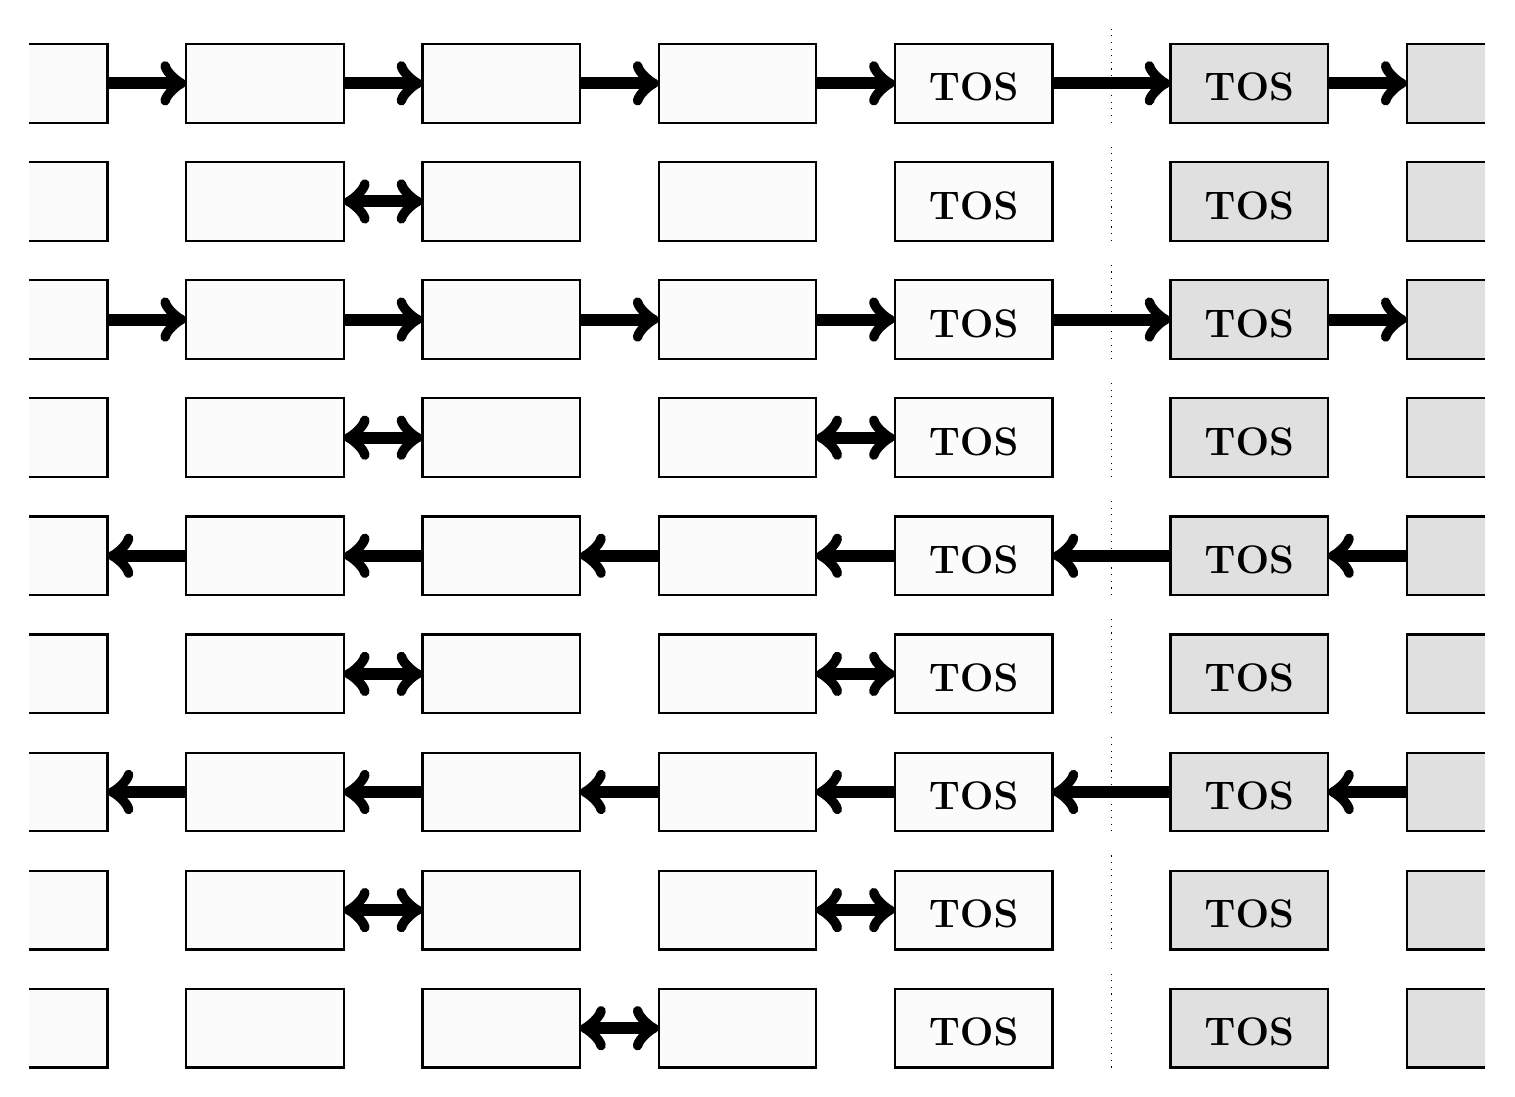
\begin{tikzpicture}
        \draw [thick, fill=gray!3]  (0,12) -- (1,12) -- (1,13) -- (0,13);%
        \draw [line width=1ex, ->]  (1,12.5)   -- (2,12.5);          %
        \draw [thick, fill=gray!3]  (2,12) rectangle (4,13);         %PS+3
        \draw [line width=1ex, ->]  (4,12.5)   -- (5,12.5);          %
        \draw [thick, fill=gray!3]  (5,12) rectangle (7,13);         %PS+2
        \draw [line width=1ex, ->]  (7,12.5)   -- (8,12.5);          %
        \draw [thick, fill=gray!3]  (8,12) rectangle (10,13);        %PS+1
        \draw [line width=1ex, ->]  (10,12.5)  -- (11,12.5);         %
        \draw [thick, fill=gray!3]  (11,12) rectangle (13,13);       %PS TOS
        \node at (12,12.45)         {\Large{\textbf{TOS}}};          %
        \draw [line width=1ex, ->]  (13,12.5)  -- (14.5,12.5);       %
        \draw [dotted]              (13.75,12) -- (13.75,13.2);      %
        \draw [thick, fill=gray!24] (14.5,12) rectangle (16.5,13);   %RS TOS
        \node at (15.5,12.45)       {\Large{\textbf{TOS}}};          %
        \draw [line width=1ex, ->]  (16.5,12.5) -- (17.5,12.5);      % 
        \draw [thick, fill=gray!24] (18.5,12)   -- (17.5,12) -- (17.5,13) -- (18.5,13);

        \draw [thick, fill=gray!3]  (0,10.5) -- (1,10.5) -- (1,11.5) -- (0,11.5);%
        %\draw [line width=1ex, --] (1,11)   -- (2,11);              %
        \draw [thick, fill=gray!3]  (2,10.5) rectangle (4,11.5);     %PS+3
        \draw [line width=1ex, <->] (4,11)   -- (5,11);              %
        \draw [thick, fill=gray!3]  (5,10.5) rectangle (7,11.5);     %PS+2
        %\draw [line width=1ex, --] (7,11)   -- (8,11);              %
        \draw [thick, fill=gray!3]  (8,10.5) rectangle (10,11.5);    %PS+1
        %\draw [line width=1ex, --] (10,11)  -- (11,11);             %
        \draw [thick, fill=gray!3]  (11,10.5) rectangle (13,11.5);   %PS TOS
        \node at (12,10.95)         {\Large{\textbf{TOS}}};          %
        %\draw [line width=1ex, --] (13,11)  -- (14.5,11);           %
        \draw [dotted]              (13.75,10.5) -- (13.75,11.7);    %
        \draw [thick, fill=gray!24] (14.5,10.5) rectangle (16.5,11.5);%RS TOS
        \node at (15.5,10.95)       {\Large{\textbf{TOS}}};          %
        %\draw [line width=1ex, --] (16.5,11) -- (17.5,11);          % 
        \draw [thick, fill=gray!24] (18.5,10.5) -- (17.5,10.5) -- (17.5,11.5) -- (18.5,11.5);

        \draw [thick, fill=gray!3]  (0,9) -- (1,9) -- (1,10) -- (0,10);%
        \draw [line width=1ex, ->]  (1,9.5)   -- (2,9.5);            %
        \draw [thick, fill=gray!3]  (2,9) rectangle (4,10);          %PS+3
        \draw [line width=1ex, ->]  (4,9.5)   -- (5,9.5);            %
        \draw [thick, fill=gray!3]  (5,9) rectangle (7,10);          %PS+2
        \draw [line width=1ex, ->]  (7,9.5)   -- (8,9.5);            %
        \draw [thick, fill=gray!3]  (8,9) rectangle (10,10);         %PS+1
        \draw [line width=1ex, ->]  (10,9.5)  -- (11,9.5);           %
        \draw [thick, fill=gray!3]  (11,9) rectangle (13,10);        %PS TOS
        \node at (12,9.45)          {\Large{\textbf{TOS}}};          %
        \draw [line width=1ex, ->]  (13,9.5)  -- (14.5,9.5);         %
        \draw [dotted]              (13.75,9) -- (13.75,10.2);       %
        \draw [thick, fill=gray!24] (14.5,9) rectangle (16.5,10);    %RS TOS
        \node at (15.5,9.45)        {\Large{\textbf{TOS}}};          %
        \draw [line width=1ex, ->]  (16.5,9.5) -- (17.5,9.5);        % 
        \draw [thick, fill=gray!24] (18.5,9)   -- (17.5,9) -- (17.5,10) -- (18.5,10);

        \draw [thick, fill=gray!3]  (0,7.5) -- (1,7.5) -- (1,8.5) -- (0,8.5);%
        %\draw [line width=1ex, --] (1,8)   -- (2,8);                %
        \draw [thick, fill=gray!3]  (2,7.5) rectangle (4,8.5);       %PS+3
        \draw [line width=1ex, <->] (4,8)   -- (5,8);                %
        \draw [thick, fill=gray!3]  (5,7.5) rectangle (7,8.5);       %PS+2
        %\draw [line width=1ex, --] (7,8)   -- (8,8);                %
        \draw [thick, fill=gray!3]  (8,7.5) rectangle (10,8.5);      %PS+1
        \draw [line width=1ex, <->] (10,8)  -- (11,8);               %
        \draw [thick, fill=gray!3]  (11,7.5) rectangle (13,8.5);     %PS TOS
        \node at (12,7.95)          {\Large{\textbf{TOS}}};          %
        %\draw [line width=1ex, --] (13,8)  -- (14.5,8);             %
        \draw [dotted]              (13.75,7.5) -- (13.75,8.7);      %
        \draw [thick, fill=gray!24] (14.5,7.5) rectangle (16.5,8.5); %RS TOS
        \node at (15.5,7.95)        {\Large{\textbf{TOS}}};          %
        %\draw [line width=1ex, --] (16.5,8) -- (17.5,8);            % 
        \draw [thick, fill=gray!24] (18.5,7.5) -- (17.5,7.5) -- (17.5,8.5) -- (18.5,8.5);

        \draw [thick, fill=gray!3]  (0,6) -- (1,6) -- (1,7) -- (0,7);%
        \draw [line width=1ex, <-]  (1,6.5)   -- (2,6.5);            %
        \draw [thick, fill=gray!3]  (2,6) rectangle (4,7);           %PS+3
        \draw [line width=1ex, <-]  (4,6.5)   -- (5,6.5);            %
        \draw [thick, fill=gray!3]  (5,6) rectangle (7,7);           %PS+2
        \draw [line width=1ex, <-]  (7,6.5)   -- (8,6.5);            %
        \draw [thick, fill=gray!3]  (8,6) rectangle (10,7);          %PS+1
        \draw [line width=1ex, <-]  (10,6.5)  -- (11,6.5);           %
        \draw [thick, fill=gray!3]  (11,6) rectangle (13,7);         %PS TOS
        \node at (12,6.45)          {\Large{\textbf{TOS}}};          %
        \draw [line width=1ex, <-]  (13,6.5)  -- (14.5,6.5);         %
        \draw [dotted]              (13.75,6) -- (13.75,7.2);        %
        \draw [thick, fill=gray!24] (14.5,6) rectangle (16.5,7);     %RS TOS
        \node at (15.5,6.45)        {\Large{\textbf{TOS}}};          %
        \draw [line width=1ex, <-]  (16.5,6.5) -- (17.5,6.5);        % 
        \draw [thick, fill=gray!24] (18.5,6)   -- (17.5,6) -- (17.5,7) -- (18.5,7);

        \draw [thick, fill=gray!3]  (0,4.5) -- (1,4.5) -- (1,5.5) -- (0,5.5);%
        %\draw [line width=1ex, --] (1,5)   -- (2,5);                %
        \draw [thick, fill=gray!3]  (2,4.5) rectangle (4,5.5);       %PS+3
        \draw [line width=1ex, <->] (4,5)   -- (5,5);                %
        \draw [thick, fill=gray!3]  (5,4.5) rectangle (7,5.5);       %PS+2
        %\draw [line width=1ex, --] (7,5)   -- (8,5);                %
        \draw [thick, fill=gray!3]  (8,4.5) rectangle (10,5.5);      %PS+1
        \draw [line width=1ex, <->] (10,5)  -- (11,5);               %
        \draw [thick, fill=gray!3]  (11,4.5) rectangle (13,5.5);     %PS TOS
        \node at (12,4.95)          {\Large{\textbf{TOS}}};          %
        %\draw [line width=1ex, --] (13,5)  -- (14.5,5);             %
        \draw [dotted]              (13.75,4.5) -- (13.75,5.7);      %
        \draw [thick, fill=gray!24] (14.5,4.5) rectangle (16.5,5.5); %RS TOS
        \node at (15.5,4.95)        {\Large{\textbf{TOS}}};          %
        %\draw [line width=1ex, --] (16.5,5) -- (17.5,5);            % 
        \draw [thick, fill=gray!24] (18.5,4.5) -- (17.5,4.5) -- (17.5,5.5) -- (18.5,5.5);

        \draw [thick, fill=gray!3]  (0,3) -- (1,3) -- (1,4) -- (0,4);%
        \draw [line width=1ex, <-]  (1,3.5)   -- (2,3.5);            %
        \draw [thick, fill=gray!3]  (2,3) rectangle (4,4);           %PS+3
        \draw [line width=1ex, <-]  (4,3.5)   -- (5,3.5);            %
        \draw [thick, fill=gray!3]  (5,3) rectangle (7,4);           %PS+2
        \draw [line width=1ex, <-]  (7,3.5)   -- (8,3.5);            %
        \draw [thick, fill=gray!3]  (8,3) rectangle (10,4);          %PS+1
        \draw [line width=1ex, <-]  (10,3.5)  -- (11,3.5);           %
        \draw [thick, fill=gray!3]  (11,3) rectangle (13,4);         %PS TOS
        \node at (12,3.45)          {\Large{\textbf{TOS}}};          %
        \draw [line width=1ex, <-]  (13,3.5)  -- (14.5,3.5);         %
        \draw [dotted]              (13.75,3) -- (13.75,4.2);        %
        \draw [thick, fill=gray!24] (14.5,3) rectangle (16.5,4);     %RS TOS
        \node at (15.5,3.45)        {\Large{\textbf{TOS}}};          %
        \draw [line width=1ex, <-]  (16.5,3.5) -- (17.5,3.5);        % 
        \draw [thick, fill=gray!24] (18.5,3)   -- (17.5,3) -- (17.5,4) -- (18.5,4);

        \draw [thick, fill=gray!3]  (0,1.5) -- (1,1.5) -- (1,2.5) -- (0,2.5);%
        %\draw [line width=1ex, --] (1,2)   -- (2,2);                %
        \draw [thick, fill=gray!3]  (2,1.5) rectangle (4,2.5);       %PS+3
        \draw [line width=1ex, <->] (4,2)   -- (5,2);                %
        \draw [thick, fill=gray!3]  (5,1.5) rectangle (7,2.5);       %PS+2
        %\draw [line width=1ex, --] (7,2)   -- (8,2);                %
        \draw [thick, fill=gray!3]  (8,1.5) rectangle (10,2.5);      %PS+1
        \draw [line width=1ex, <->] (10,2)  -- (11,2);               %
        \draw [thick, fill=gray!3]  (11,1.5) rectangle (13,2.5);     %PS TOS
        \node at (12,1.95)          {\Large{\textbf{TOS}}};          %
        %\draw [line width=1ex, --] (13,2)  -- (14.5,2);             %
        \draw [dotted]              (13.75,1.5) -- (13.75,2.7);      %
        \draw [thick, fill=gray!24] (14.5,1.5) rectangle (16.5,2.5); %RS TOS
        \node at (15.5,1.95)        {\Large{\textbf{TOS}}};          %
        %\draw [line width=1ex, --] (16.5,2) -- (17.5,2);            % 
        \draw [thick, fill=gray!24] (18.5,1.5) -- (17.5,1.5) -- (17.5,2.5) -- (18.5,2.5);

        \draw [thick, fill=gray!3]  (0,0) -- (1,0) -- (1,1) -- (0,1);%
        %\draw [line width=1ex, --] (1,0.5) -- (2,0.5);              %
        \draw [thick, fill=gray!3]  (2,0) rectangle (4,1);           %PS+3
        %\draw [line width=1ex, --] (4,0.5) -- (5,0.5);              %
        \draw [thick, fill=gray!3]  (5,0) rectangle (7,1);           %PS+2
        \draw [line width=1ex, <->] (7,0.5) -- (8,0.5);              %
        \draw [thick, fill=gray!3]  (8,0) rectangle (10,1);          %PS+1
        %\draw [line width=1ex, --] (10,0.5) -- (11,0.5);            %
        \draw [thick, fill=gray!3]  (11,0) rectangle (13,1);         %PS TOS
        \node at (12,0.45)          {\Large{\textbf{TOS}}};          %
        %\draw [line width=1ex, --] (13,0.5)  -- (14.5,0.5);         %
        \draw [dotted]              (13.75,0) -- (13.75,1.2);        %
        \draw [thick, fill=gray!24] (14.5,0) rectangle (16.5,1);     %RS TOS
        \node at (15.5,0.45)        {\Large{\textbf{TOS}}};          %
        %\draw [line width=1ex, --] (16.5,0.5) -- (17.5,0.5);        % 
        \draw [thick, fill=gray!24] (18.5,0) -- (17.5,0) -- (17.5,1) -- (18.5,1);
      \end{tikzpicture}
    }} &
    \multicolumn{1}{m{4.25em}|}{
    \makecell[c]{ 
      \texttt{0x06AB} \\ 
      \texttt{0x0580} \\ 
      \texttt{0x06AB} \\ 
      \texttt{0x0598} \\ 
      \texttt{0x0755} \\ 
      \texttt{0x0598} \\ 
      \texttt{0x0755} \\ 
      \texttt{0x0598} \\ 
      \texttt{0x0460}
    }} \\ \hline

    %-2ROT
    \texttt{-2ROT} &
    ( x1 x2 x3 x4 x5 x6 -- x5 x6 x1 x2 x3 x4 ) &
    \multicolumn{1}{m{21.35em}|}{
    \scalebox{0.4} {
      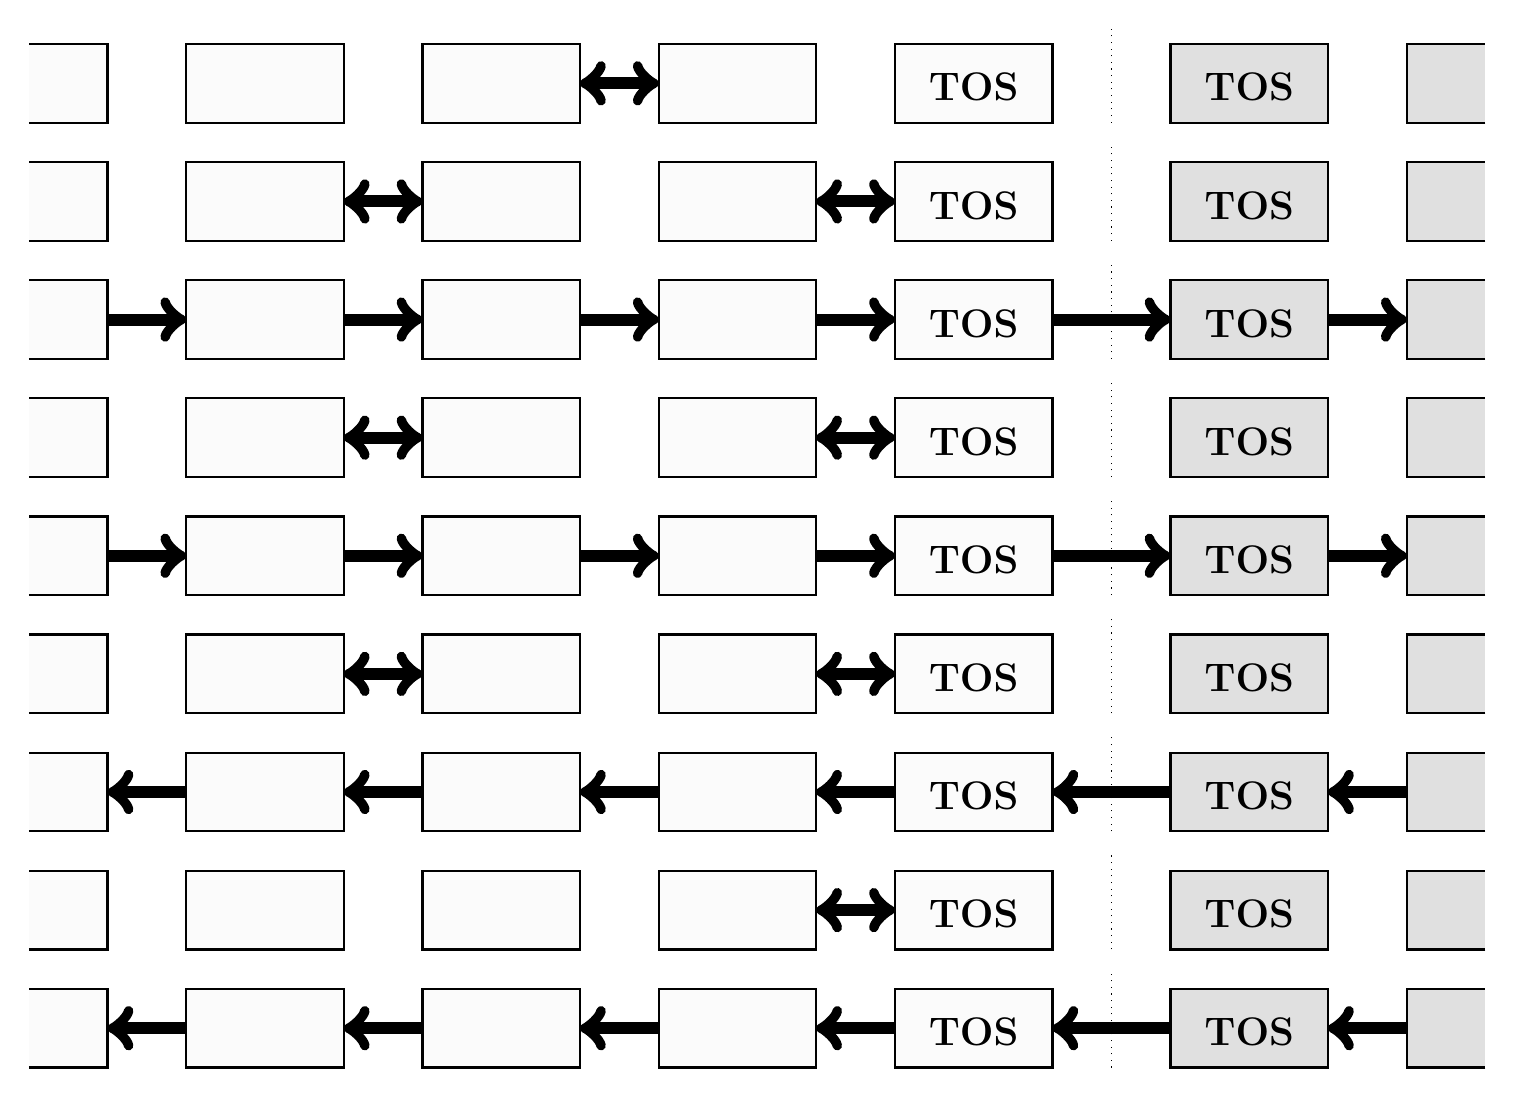
\begin{tikzpicture}
        \draw [thick, fill=gray!3]  (0,12) -- (1,12) -- (1,13) -- (0,13);%
        %\draw [line width=1ex, --] (1,12.5)   -- (2,12.5);          %
        \draw [thick, fill=gray!3]  (2,12) rectangle (4,13);         %PS+3
        %\draw [line width=1ex, --] (4,12.5)   -- (5,12.5);          %
        \draw [thick, fill=gray!3]  (5,12) rectangle (7,13);         %PS+2
        \draw [line width=1ex, <->] (7,12.5)   -- (8,12.5);          %
        \draw [thick, fill=gray!3]  (8,12) rectangle (10,13);        %PS+1
        %\draw [line width=1ex, --] (10,12.5)  -- (11,12.5);         %
        \draw [thick, fill=gray!3]  (11,12) rectangle (13,13);       %PS TOS
        \node at (12,12.45)         {\Large{\textbf{TOS}}};          %
        %\draw [line width=1ex, --] (13,12.5)  -- (14.5,12.5);       %
        \draw [dotted]              (13.75,12) -- (13.75,13.2);      %
        \draw [thick, fill=gray!24] (14.5,12) rectangle (16.5,13);   %RS TOS
        \node at (15.5,12.45)       {\Large{\textbf{TOS}}};          %
        %\draw [line width=1ex, --] (16.5,12.5) -- (17.5,12.5);      % 
        \draw [thick, fill=gray!24] (18.5,12)   -- (17.5,12) -- (17.5,13) -- (18.5,13);

        \draw [thick, fill=gray!3]  (0,10.5) -- (1,10.5) -- (1,11.5) -- (0,11.5);%
        %\draw [line width=1ex, --] (1,11)   -- (2,11);              %
        \draw [thick, fill=gray!3]  (2,10.5) rectangle (4,11.5);     %PS+3
        \draw [line width=1ex, <->] (4,11)   -- (5,11);              %
        \draw [thick, fill=gray!3]  (5,10.5) rectangle (7,11.5);     %PS+2
        %\draw [line width=1ex, --] (7,11)   -- (8,11);              %
        \draw [thick, fill=gray!3]  (8,10.5) rectangle (10,11.5);    %PS+1
        \draw [line width=1ex, <->] (10,11)  -- (11,11);             %
        \draw [thick, fill=gray!3]  (11,10.5) rectangle (13,11.5);   %PS TOS
        \node at (12,10.95)         {\Large{\textbf{TOS}}};          %
        %\draw [line width=1ex, --] (13,11)  -- (14.5,11);           %
        \draw [dotted]              (13.75,10.5) -- (13.75,11.7);    %
        \draw [thick, fill=gray!24] (14.5,10.5) rectangle (16.5,11.5);%RS TOS
        \node at (15.5,10.95)       {\Large{\textbf{TOS}}};          %
        %\draw [line width=1ex, --] (16.5,11) -- (17.5,11);          % 
        \draw [thick, fill=gray!24] (18.5,10.5) -- (17.5,10.5) -- (17.5,11.5) -- (18.5,11.5);

        \draw [thick, fill=gray!3]  (0,9) -- (1,9) -- (1,10) -- (0,10);%
        \draw [line width=1ex, ->]  (1,9.5)   -- (2,9.5);            %
        \draw [thick, fill=gray!3]  (2,9) rectangle (4,10);          %PS+3
        \draw [line width=1ex, ->]  (4,9.5)   -- (5,9.5);            %
        \draw [thick, fill=gray!3]  (5,9) rectangle (7,10);          %PS+2
        \draw [line width=1ex, ->]  (7,9.5)   -- (8,9.5);            %
        \draw [thick, fill=gray!3]  (8,9) rectangle (10,10);         %PS+1
        \draw [line width=1ex, ->]  (10,9.5)  -- (11,9.5);           %
        \draw [thick, fill=gray!3]  (11,9) rectangle (13,10);        %PS TOS
        \node at (12,9.45)          {\Large{\textbf{TOS}}};          %
        \draw [line width=1ex, ->]  (13,9.5)  -- (14.5,9.5);         %
        \draw [dotted]              (13.75,9) -- (13.75,10.2);       %
        \draw [thick, fill=gray!24] (14.5,9) rectangle (16.5,10);    %RS TOS
        \node at (15.5,9.45)        {\Large{\textbf{TOS}}};          %
        \draw [line width=1ex, ->]  (16.5,9.5) -- (17.5,9.5);        % 
        \draw [thick, fill=gray!24] (18.5,9)   -- (17.5,9) -- (17.5,10) -- (18.5,10);

        \draw [thick, fill=gray!3]  (0,7.5) -- (1,7.5) -- (1,8.5) -- (0,8.5);%
        %\draw [line width=1ex, --] (1,8)   -- (2,8);                %
        \draw [thick, fill=gray!3]  (2,7.5) rectangle (4,8.5);       %PS+3
        \draw [line width=1ex, <->] (4,8)   -- (5,8);                %
        \draw [thick, fill=gray!3]  (5,7.5) rectangle (7,8.5);       %PS+2
        %\draw [line width=1ex, --] (7,8)   -- (8,8);                %
        \draw [thick, fill=gray!3]  (8,7.5) rectangle (10,8.5);      %PS+1
        \draw [line width=1ex, <->] (10,8)  -- (11,8);               %
        \draw [thick, fill=gray!3]  (11,7.5) rectangle (13,8.5);     %PS TOS
        \node at (12,7.95)          {\Large{\textbf{TOS}}};          %
        %\draw [line width=1ex, --] (13,8)  -- (14.5,8);             %
        \draw [dotted]              (13.75,7.5) -- (13.75,8.7);      %
        \draw [thick, fill=gray!24] (14.5,7.5) rectangle (16.5,8.5); %RS TOS
        \node at (15.5,7.95)        {\Large{\textbf{TOS}}};          %
        %\draw [line width=1ex, --] (16.5,8) -- (17.5,8);            % 
        \draw [thick, fill=gray!24] (18.5,7.5) -- (17.5,7.5) -- (17.5,8.5) -- (18.5,8.5);

        \draw [thick, fill=gray!3]  (0,6) -- (1,6) -- (1,7) -- (0,7);%
        \draw [line width=1ex, ->] (1,6.5)   -- (2,6.5);             %
        \draw [thick, fill=gray!3]  (2,6) rectangle (4,7);           %PS+3
        \draw [line width=1ex, ->] (4,6.5)   -- (5,6.5);             %
        \draw [thick, fill=gray!3]  (5,6) rectangle (7,7);           %PS+2
        \draw [line width=1ex, ->] (7,6.5)   -- (8,6.5);             %
        \draw [thick, fill=gray!3]  (8,6) rectangle (10,7);          %PS+1
        \draw [line width=1ex, ->] (10,6.5)  -- (11,6.5);            %
        \draw [thick, fill=gray!3]  (11,6) rectangle (13,7);         %PS TOS
        \node at (12,6.45)          {\Large{\textbf{TOS}}};          %
        \draw [line width=1ex, ->] (13,6.5)  -- (14.5,6.5);          %
        \draw [dotted]              (13.75,6) -- (13.75,7.2);        %
        \draw [thick, fill=gray!24] (14.5,6) rectangle (16.5,7);     %RS TOS
        \node at (15.5,6.45)        {\Large{\textbf{TOS}}};          %
        \draw [line width=1ex, ->]  (16.5,6.5) -- (17.5,6.5);        % 
        \draw [thick, fill=gray!24] (18.5,6)   -- (17.5,6) -- (17.5,7) -- (18.5,7);

        \draw [thick, fill=gray!3]  (0,4.5) -- (1,4.5) -- (1,5.5) -- (0,5.5);%
        %\draw [line width=1ex, --] (1,5)   -- (2,5);                %
        \draw [thick, fill=gray!3]  (2,4.5) rectangle (4,5.5);       %PS+3
        \draw [line width=1ex, <->] (4,5)   -- (5,5);                %
        \draw [thick, fill=gray!3]  (5,4.5) rectangle (7,5.5);       %PS+2
        %\draw [line width=1ex, --] (7,5)   -- (8,5);                %
        \draw [thick, fill=gray!3]  (8,4.5) rectangle (10,5.5);      %PS+1
        \draw [line width=1ex, <->] (10,5)  -- (11,5);               %
        \draw [thick, fill=gray!3]  (11,4.5) rectangle (13,5.5);     %PS TOS
        \node at (12,4.95)          {\Large{\textbf{TOS}}};          %
        %\draw [line width=1ex, --] (13,5)  -- (14.5,5);             %
        \draw [dotted]              (13.75,4.5) -- (13.75,5.7);      %
        \draw [thick, fill=gray!24] (14.5,4.5) rectangle (16.5,5.5); %RS TOS
        \node at (15.5,4.95)        {\Large{\textbf{TOS}}};          %
        %\draw [line width=1ex, --] (16.5,5) -- (17.5,5);            % 
        \draw [thick, fill=gray!24] (18.5,4.5) -- (17.5,4.5) -- (17.5,5.5) -- (18.5,5.5);

        \draw [thick, fill=gray!3]  (0,3) -- (1,3) -- (1,4) -- (0,4);%
        \draw [line width=1ex, <-]  (1,3.5)   -- (2,3.5);            %
        \draw [thick, fill=gray!3]  (2,3) rectangle (4,4);           %PS+3
        \draw [line width=1ex, <-]  (4,3.5)   -- (5,3.5);            %
        \draw [thick, fill=gray!3]  (5,3) rectangle (7,4);           %PS+2
        \draw [line width=1ex, <-]  (7,3.5)   -- (8,3.5);            %
        \draw [thick, fill=gray!3]  (8,3) rectangle (10,4);          %PS+1
        \draw [line width=1ex, <-]  (10,3.5)  -- (11,3.5);           %
        \draw [thick, fill=gray!3]  (11,3) rectangle (13,4);         %PS TOS
        \node at (12,3.45)          {\Large{\textbf{TOS}}};          %
        \draw [line width=1ex, <-]  (13,3.5)  -- (14.5,3.5);         %
        \draw [dotted]              (13.75,3) -- (13.75,4.2);        %
        \draw [thick, fill=gray!24] (14.5,3) rectangle (16.5,4);     %RS TOS
        \node at (15.5,3.45)        {\Large{\textbf{TOS}}};          %
        \draw [line width=1ex, <-]  (16.5,3.5) -- (17.5,3.5);        % 
        \draw [thick, fill=gray!24] (18.5,3)   -- (17.5,3) -- (17.5,4) -- (18.5,4);

        \draw [thick, fill=gray!3]  (0,1.5) -- (1,1.5) -- (1,2.5) -- (0,2.5);%
        %\draw [line width=1ex, --] (1,2)   -- (2,2);                %
        \draw [thick, fill=gray!3]  (2,1.5) rectangle (4,2.5);       %PS+3
        %\draw [line width=1ex, --] (4,2)   -- (5,2);                %
        \draw [thick, fill=gray!3]  (5,1.5) rectangle (7,2.5);       %PS+2
        %\draw [line width=1ex, --] (7,2)   -- (8,2);                %
        \draw [thick, fill=gray!3]  (8,1.5) rectangle (10,2.5);      %PS+1
        \draw [line width=1ex, <->] (10,2)  -- (11,2);               %
        \draw [thick, fill=gray!3]  (11,1.5) rectangle (13,2.5);     %PS TOS
        \node at (12,1.95)          {\Large{\textbf{TOS}}};          %
        %\draw [line width=1ex, --] (13,2)  -- (14.5,2);             %
        \draw [dotted]              (13.75,1.5) -- (13.75,2.7);      %
        \draw [thick, fill=gray!24] (14.5,1.5) rectangle (16.5,2.5); %RS TOS
        \node at (15.5,1.95)        {\Large{\textbf{TOS}}};          %
        %\draw [line width=1ex, --] (16.5,2) -- (17.5,2);            % 
        \draw [thick, fill=gray!24] (18.5,1.5) -- (17.5,1.5) -- (17.5,2.5) -- (18.5,2.5);

        \draw [thick, fill=gray!3]  (0,0) -- (1,0) -- (1,1) -- (0,1);%
        \draw [line width=1ex, <-] (1,0.5) -- (2,0.5);               %
        \draw [thick, fill=gray!3]  (2,0) rectangle (4,1);           %PS+3
        \draw [line width=1ex, <-] (4,0.5) -- (5,0.5);               %
        \draw [thick, fill=gray!3]  (5,0) rectangle (7,1);           %PS+2
        \draw [line width=1ex, <-] (7,0.5) -- (8,0.5);               %
        \draw [thick, fill=gray!3]  (8,0) rectangle (10,1);          %PS+1
        \draw [line width=1ex, <-] (10,0.5) -- (11,0.5);             %
        \draw [thick, fill=gray!3]  (11,0) rectangle (13,1);         %PS TOS
        \node at (12,0.45)          {\Large{\textbf{TOS}}};          %
        \draw [line width=1ex, <-] (13,0.5)  -- (14.5,0.5);          %
        \draw [dotted]              (13.75,0) -- (13.75,1.2);        %
        \draw [thick, fill=gray!24] (14.5,0) rectangle (16.5,1);     %RS TOS
        \node at (15.5,0.45)        {\Large{\textbf{TOS}}};          %
        \draw [line width=1ex, <-] (16.5,0.5) -- (17.5,0.5);         % 
        \draw [thick, fill=gray!24] (18.5,0) -- (17.5,0) -- (17.5,1) -- (18.5,1);
      \end{tikzpicture}
    }} &
    \multicolumn{1}{m{4.25em}|}{
    \makecell[c]{ 
      \texttt{0x0460} \\ 
      \texttt{0x0598} \\ 
      \texttt{0x06AB} \\ 
      \texttt{0x0598} \\ 
      \texttt{0x06AB} \\ 
      \texttt{0x0598} \\ 
      \texttt{0x0755} \\ 
      \texttt{0x0418} \\ 
      \texttt{0x0755}
    }} \\ \hline

    %2RDROP
    \texttt{2RDROP} &
      ( R: x1 x2 -- ) &
    \multicolumn{1}{m{21.35em}|}{
    \scalebox{0.4} {
      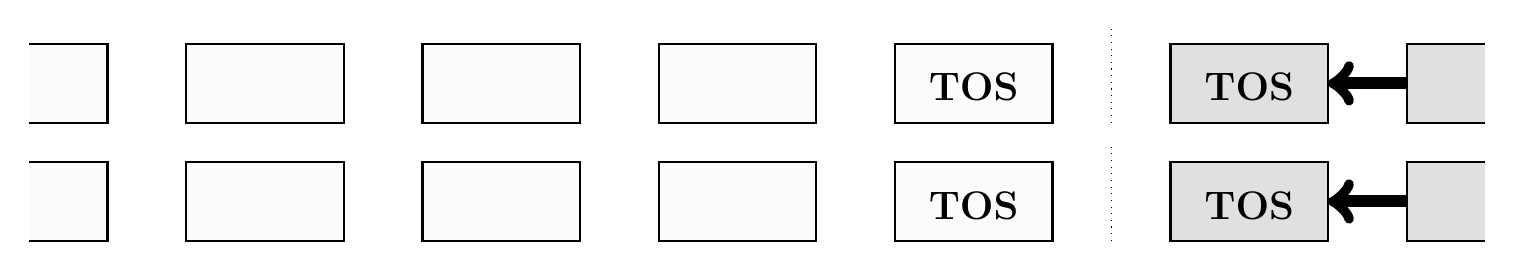
\begin{tikzpicture}
        \draw [thick, fill=gray!3]  (0,1.5) -- (1,1.5) -- (1,2.5) -- (0,2.5);%
        %\draw [line width=1ex, --] (1,2)   -- (2,2);                %
        \draw [thick, fill=gray!3]  (2,1.5) rectangle (4,2.5);       %PS+3
        %\draw [line width=1ex, --] (4,2)   -- (5,2);                %
        \draw [thick, fill=gray!3]  (5,1.5) rectangle (7,2.5);       %PS+2
        %\draw [line width=1ex, --] (7,2)   -- (8,2);                %
        \draw [thick, fill=gray!3]  (8,1.5) rectangle (10,2.5);      %PS+1
        %\draw [line width=1ex, --] (10,2)  -- (11,2);               %
        \draw [thick, fill=gray!3]  (11,1.5) rectangle (13,2.5);     %PS TOS
        \node at (12,1.95)          {\Large{\textbf{TOS}}};          %
        %\draw [line width=1ex, --] (13,2)  -- (14.5,2);             %
        \draw [dotted]              (13.75,1.5) -- (13.75,2.7);      %
        \draw [thick, fill=gray!24] (14.5,1.5) rectangle (16.5,2.5); %RS TOS
        \node at (15.5,1.95)        {\Large{\textbf{TOS}}};          %
        \draw [line width=1ex, <-]  (16.5,2) -- (17.5,2);            % 
        \draw [thick, fill=gray!24] (18.5,1.5) -- (17.5,1.5) -- (17.5,2.5) -- (18.5,2.5);

        \draw [thick, fill=gray!3]  (0,0) -- (1,0) -- (1,1) -- (0,1);%
        %\draw [line width=1ex, --] (1,0.5) -- (2,0.5);              %
        \draw [thick, fill=gray!3]  (2,0) rectangle (4,1);           %PS+3
        %\draw [line width=1ex, --] (4,0.5) -- (5,0.5);              %
        \draw [thick, fill=gray!3]  (5,0) rectangle (7,1);           %PS+2
        %\draw [line width=1ex, --] (7,0.5) -- (8,0.5);              %
        \draw [thick, fill=gray!3]  (8,0) rectangle (10,1);          %PS+1
        %\draw [line width=1ex, --] (10,0.5) -- (11,0.5);            %
        \draw [thick, fill=gray!3]  (11,0) rectangle (13,1);         %PS TOS
        \node at (12,0.45)          {\Large{\textbf{TOS}}};          %
        %\draw [line width=1ex, --] (13,0.5)  -- (14.5,0.5);         %
        \draw [dotted]              (13.75,0) -- (13.75,1.2);        %
        \draw [thick, fill=gray!24] (14.5,0) rectangle (16.5,1);     %RS TOS
        \node at (15.5,0.45)        {\Large{\textbf{TOS}}};          %
        \draw [line width=1ex, <-]  (16.5,0.5) -- (17.5,0.5);        % 
        \draw [thick, fill=gray!24] (18.5,0) -- (17.5,0) -- (17.5,1) -- (18.5,1);
      \end{tikzpicture}
    }} &
    \multicolumn{1}{m{4.25em}|}{
    \makecell[c]{ 
      \texttt{0x0401} \\ 
      \texttt{0x0401}
    }} \\ \hline

    %2RDUP
    \texttt{2RDUP} &
    ( R: x1 x2 -- x1 x2 x1 x2 ) &
    \multicolumn{1}{m{21.35em}|}{
    \scalebox{0.4} {
      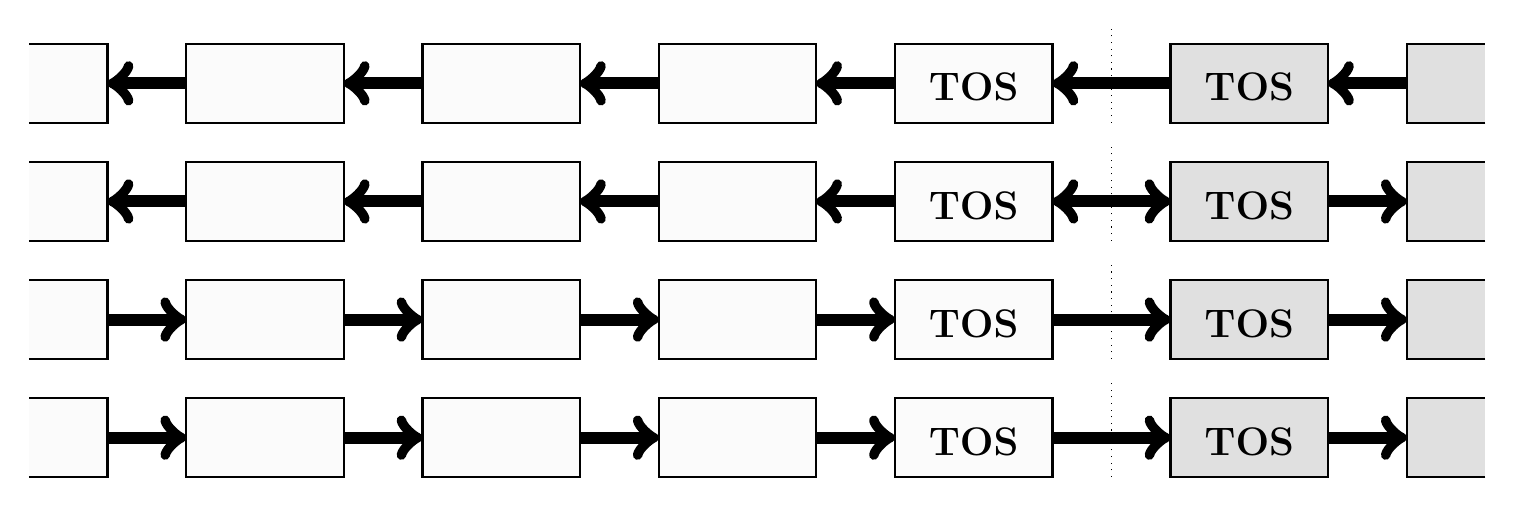
\begin{tikzpicture}
        \draw [thick, fill=gray!3]  (0,4.5) -- (1,4.5) -- (1,5.5) -- (0,5.5);%
        \draw [line width=1ex, <-]  (1,5)   -- (2,5);                %
        \draw [thick, fill=gray!3]  (2,4.5) rectangle (4,5.5);       %PS+3
        \draw [line width=1ex, <-]  (4,5)   -- (5,5);                %
        \draw [thick, fill=gray!3]  (5,4.5) rectangle (7,5.5);       %PS+2
        \draw [line width=1ex, <-]  (7,5)   -- (8,5);                %
        \draw [thick, fill=gray!3]  (8,4.5) rectangle (10,5.5);      %PS+1
        \draw [line width=1ex, <-]  (10,5)  -- (11,5);               %
        \draw [thick, fill=gray!3]  (11,4.5) rectangle (13,5.5);     %PS TOS
        \node at (12,4.95)          {\Large{\textbf{TOS}}};          %
        \draw [line width=1ex, <-]  (13,5)  -- (14.5,5);             %
        \draw [dotted]              (13.75,4.5) -- (13.75,5.7);      %
        \draw [thick, fill=gray!24] (14.5,4.5) rectangle (16.5,5.5); %RS TOS
        \node at (15.5,4.95)        {\Large{\textbf{TOS}}};          %
        \draw [line width=1ex, <-]  (16.5,5) -- (17.5,5);            % 
        \draw [thick, fill=gray!24] (18.5,4.5) -- (17.5,4.5) -- (17.5,5.5) -- (18.5,5.5);

        \draw [thick, fill=gray!3]  (0,3) -- (1,3) -- (1,4) -- (0,4);%
        \draw [line width=1ex, <-]  (1,3.5)   -- (2,3.5);            %
        \draw [thick, fill=gray!3]  (2,3) rectangle (4,4);           %PS+3
        \draw [line width=1ex, <-]  (4,3.5)   -- (5,3.5);            %
        \draw [thick, fill=gray!3]  (5,3) rectangle (7,4);           %PS+2
        \draw [line width=1ex, <-]  (7,3.5)   -- (8,3.5);            %
        \draw [thick, fill=gray!3]  (8,3) rectangle (10,4);          %PS+1
        \draw [line width=1ex, <-]  (10,3.5)  -- (11,3.5);           %
        \draw [thick, fill=gray!3]  (11,3) rectangle (13,4);         %PS TOS
        \node at (12,3.45)          {\Large{\textbf{TOS}}};          %
        \draw [line width=1ex, <->] (13,3.5)  -- (14.5,3.5);         %
        \draw [dotted]              (13.75,3) -- (13.75,4.2);        %
        \draw [thick, fill=gray!24] (14.5,3) rectangle (16.5,4);     %RS TOS
        \node at (15.5,3.45)        {\Large{\textbf{TOS}}};          %
        \draw [line width=1ex, ->]  (16.5,3.5) -- (17.5,3.5);        % 
        \draw [thick, fill=gray!24] (18.5,3)   -- (17.5,3) -- (17.5,4) -- (18.5,4);

        \draw [thick, fill=gray!3]  (0,1.5) -- (1,1.5) -- (1,2.5) -- (0,2.5);%
        \draw [line width=1ex, ->]  (1,2)   -- (2,2);                %
        \draw [thick, fill=gray!3]  (2,1.5) rectangle (4,2.5);       %PS+3
        \draw [line width=1ex, ->]  (4,2)   -- (5,2);                %
        \draw [thick, fill=gray!3]  (5,1.5) rectangle (7,2.5);       %PS+2
        \draw [line width=1ex, ->]  (7,2)   -- (8,2);                %
        \draw [thick, fill=gray!3]  (8,1.5) rectangle (10,2.5);      %PS+1
        \draw [line width=1ex, ->]  (10,2)  -- (11,2);               %
        \draw [thick, fill=gray!3]  (11,1.5) rectangle (13,2.5);     %PS TOS
        \node at (12,1.95)          {\Large{\textbf{TOS}}};          %
        \draw [line width=1ex, ->]  (13,2)  -- (14.5,2);             %
        \draw [dotted]              (13.75,1.5) -- (13.75,2.7);      %
        \draw [thick, fill=gray!24] (14.5,1.5) rectangle (16.5,2.5); %RS TOS
        \node at (15.5,1.95)        {\Large{\textbf{TOS}}};          %
        \draw [line width=1ex, ->]  (16.5,2) -- (17.5,2);            % 
        \draw [thick, fill=gray!24] (18.5,1.5) -- (17.5,1.5) -- (17.5,2.5) -- (18.5,2.5);

        \draw [thick, fill=gray!3]  (0,0) -- (1,0) -- (1,1) -- (0,1);%
        \draw [line width=1ex, ->]  (1,0.5) -- (2,0.5);              %
        \draw [thick, fill=gray!3]  (2,0) rectangle (4,1);           %PS+3
        \draw [line width=1ex, ->]  (4,0.5) -- (5,0.5);              %
        \draw [thick, fill=gray!3]  (5,0) rectangle (7,1);           %PS+2
        \draw [line width=1ex, ->]  (7,0.5) -- (8,0.5);              %
        \draw [thick, fill=gray!3]  (8,0) rectangle (10,1);          %PS+1
        \draw [line width=1ex, ->]  (10,0.5) -- (11,0.5);            %
        \draw [thick, fill=gray!3]  (11,0) rectangle (13,1);         %PS TOS
        \node at (12,0.45)          {\Large{\textbf{TOS}}};          %
        \draw [line width=1ex, ->]  (13,0.5)  -- (14.5,0.5);         %
        \draw [dotted]              (13.75,0) -- (13.75,1.2);        %
        \draw [thick, fill=gray!24] (14.5,0) rectangle (16.5,1);     %RS TOS
        \node at (15.5,0.45)        {\Large{\textbf{TOS}}};          %
        \draw [line width=1ex, ->]  (16.5,0.5) -- (17.5,0.5);        % 
        \draw [thick, fill=gray!24] (18.5,0) -- (17.5,0) -- (17.5,1) -- (18.5,1);
      \end{tikzpicture}
    }} &
    \multicolumn{1}{m{4.25em}|}{
    \makecell[c]{ 
      \texttt{0x0755} \\ 
      \texttt{0x0757} \\ 
      \texttt{0x06AB} \\ 
      \texttt{0x06AB}
    }} \\ \hline

    %2>R
    \texttt{2>R} &
    \multicolumn{1}{m{18.3em}|}{
    \makecell[c]{ 
      ( x1 x2 -- )\\
      ( R: -- x1 x2 )
    }} &
    \multicolumn{1}{m{21.35em}|}{
    \scalebox{0.4} {
      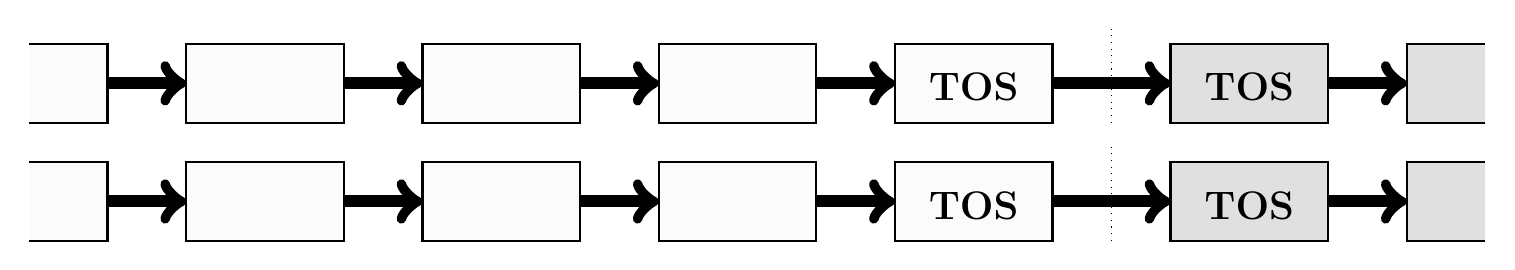
\begin{tikzpicture}
        \draw [thick, fill=gray!3]  (0,1.5) -- (1,1.5) -- (1,2.5) -- (0,2.5);%
        \draw [line width=1ex, ->]  (1,2)   -- (2,2);                %
        \draw [thick, fill=gray!3]  (2,1.5) rectangle (4,2.5);       %PS+3
        \draw [line width=1ex, ->]  (4,2)   -- (5,2);                %
        \draw [thick, fill=gray!3]  (5,1.5) rectangle (7,2.5);       %PS+2
        \draw [line width=1ex, ->]  (7,2)   -- (8,2);                %
        \draw [thick, fill=gray!3]  (8,1.5) rectangle (10,2.5);      %PS+1
        \draw [line width=1ex, ->]  (10,2)  -- (11,2);               %
        \draw [thick, fill=gray!3]  (11,1.5) rectangle (13,2.5);     %PS TOS
        \node at (12,1.95)          {\Large{\textbf{TOS}}};          %
        \draw [line width=1ex, ->]  (13,2)  -- (14.5,2);             %
        \draw [dotted]              (13.75,1.5) -- (13.75,2.7);      %
        \draw [thick, fill=gray!24] (14.5,1.5) rectangle (16.5,2.5); %RS TOS
        \node at (15.5,1.95)        {\Large{\textbf{TOS}}};          %
        \draw [line width=1ex, ->]  (16.5,2) -- (17.5,2);            % 
        \draw [thick, fill=gray!24] (18.5,1.5) -- (17.5,1.5) -- (17.5,2.5) -- (18.5,2.5);

        \draw [thick, fill=gray!3]  (0,0) -- (1,0) -- (1,1) -- (0,1);%
        \draw [line width=1ex, ->]  (1,0.5) -- (2,0.5);              %
        \draw [thick, fill=gray!3]  (2,0) rectangle (4,1);           %PS+3
        \draw [line width=1ex, ->]  (4,0.5) -- (5,0.5);              %
        \draw [thick, fill=gray!3]  (5,0) rectangle (7,1);           %PS+2
        \draw [line width=1ex, ->]  (7,0.5) -- (8,0.5);              %
        \draw [thick, fill=gray!3]  (8,0) rectangle (10,1);          %PS+1
        \draw [line width=1ex, ->]  (10,0.5) -- (11,0.5);            %
        \draw [thick, fill=gray!3]  (11,0) rectangle (13,1);         %PS TOS
        \node at (12,0.45)          {\Large{\textbf{TOS}}};          %
        \draw [line width=1ex, ->]  (13,0.5)  -- (14.5,0.5);         %
        \draw [dotted]              (13.75,0) -- (13.75,1.2);        %
        \draw [thick, fill=gray!24] (14.5,0) rectangle (16.5,1);     %RS TOS
        \node at (15.5,0.45)        {\Large{\textbf{TOS}}};          %
        \draw [line width=1ex, ->]  (16.5,0.5) -- (17.5,0.5);        % 
        \draw [thick, fill=gray!24] (18.5,0) -- (17.5,0) -- (17.5,1) -- (18.5,1);
      \end{tikzpicture}
    }} &
    \multicolumn{1}{m{4.25em}|}{
    \makecell[c]{ 
      \texttt{0x06AB} \\ 
      \texttt{0x06AB}
    }} \\ \hline

    %2R@
    \texttt{2R@} &
    \multicolumn{1}{m{18.3em}|}{
    \makecell[c]{ 
      ( -- x1 x2 )\\
      ( R: x1 x2 -- x1 x2 )
    }} &
    \multicolumn{1}{m{21.35em}|}{
    \scalebox{0.4} {
      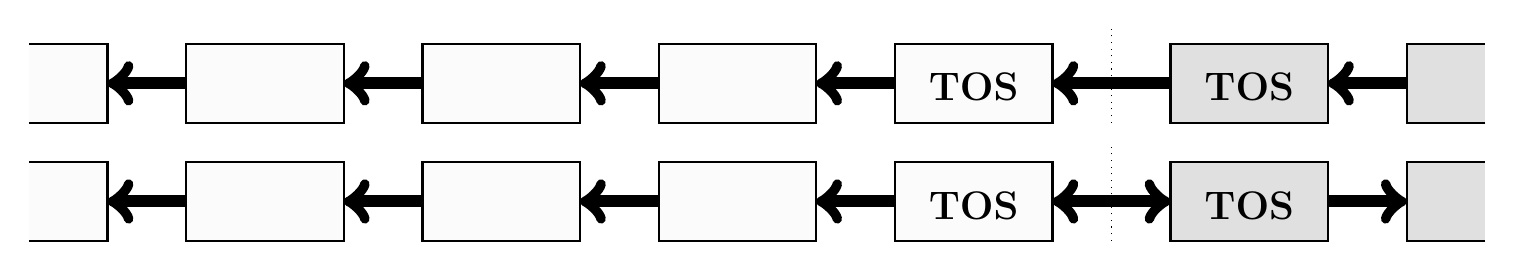
\begin{tikzpicture}
        \draw [thick, fill=gray!3]  (0,1.5) -- (1,1.5) -- (1,2.5) -- (0,2.5);%
        \draw [line width=1ex, <-]  (1,2)   -- (2,2);                %
        \draw [thick, fill=gray!3]  (2,1.5) rectangle (4,2.5);       %PS+3
        \draw [line width=1ex, <-]  (4,2)   -- (5,2);                %
        \draw [thick, fill=gray!3]  (5,1.5) rectangle (7,2.5);       %PS+2
        \draw [line width=1ex, <-]  (7,2)   -- (8,2);                %
        \draw [thick, fill=gray!3]  (8,1.5) rectangle (10,2.5);      %PS+1
        \draw [line width=1ex, <-]  (10,2)  -- (11,2);               %
        \draw [thick, fill=gray!3]  (11,1.5) rectangle (13,2.5);     %PS TOS
        \node at (12,1.95)          {\Large{\textbf{TOS}}};          %
        \draw [line width=1ex, <-]  (13,2)  -- (14.5,2);             %
        \draw [dotted]              (13.75,1.5) -- (13.75,2.7);      %
        \draw [thick, fill=gray!24] (14.5,1.5) rectangle (16.5,2.5); %RS TOS
        \node at (15.5,1.95)        {\Large{\textbf{TOS}}};          %
        \draw [line width=1ex, <-]  (16.5,2) -- (17.5,2);            % 
        \draw [thick, fill=gray!24] (18.5,1.5) -- (17.5,1.5) -- (17.5,2.5) -- (18.5,2.5);

        \draw [thick, fill=gray!3]  (0,0) -- (1,0) -- (1,1) -- (0,1);%
        \draw [line width=1ex, <-]  (1,0.5) -- (2,0.5);              %
        \draw [thick, fill=gray!3]  (2,0) rectangle (4,1);           %PS+3
        \draw [line width=1ex, <-]  (4,0.5) -- (5,0.5);              %
        \draw [thick, fill=gray!3]  (5,0) rectangle (7,1);           %PS+2
        \draw [line width=1ex, <-]  (7,0.5) -- (8,0.5);              %
        \draw [thick, fill=gray!3]  (8,0) rectangle (10,1);          %PS+1
        \draw [line width=1ex, <-]  (10,0.5) -- (11,0.5);            %
        \draw [thick, fill=gray!3]  (11,0) rectangle (13,1);         %PS TOS
        \node at (12,0.45)          {\Large{\textbf{TOS}}};          %
        \draw [line width=1ex, <->] (13,0.5)  -- (14.5,0.5);         %
        \draw [dotted]              (13.75,0) -- (13.75,1.2);        %
        \draw [thick, fill=gray!24] (14.5,0) rectangle (16.5,1);     %RS TOS
        \node at (15.5,0.45)        {\Large{\textbf{TOS}}};          %
        \draw [line width=1ex, ->]  (16.5,0.5) -- (17.5,0.5);        % 
        \draw [thick, fill=gray!24] (18.5,0) -- (17.5,0) -- (17.5,1) -- (18.5,1);
      \end{tikzpicture}
    }} &
    \multicolumn{1}{m{4.25em}|}{
    \makecell[c]{ 
      \texttt{0x0755} \\ 
      \texttt{0x0757}
    }} \\ \hline

    %2R>
    \texttt{2R>} &
    \multicolumn{1}{m{18.3em}|}{
    \makecell[c]{ 
      ( -- x1 x2 )\\
      ( R: x1 x2 -- )
    }} &
    \multicolumn{1}{m{21.35em}|}{
    \scalebox{0.4} {
      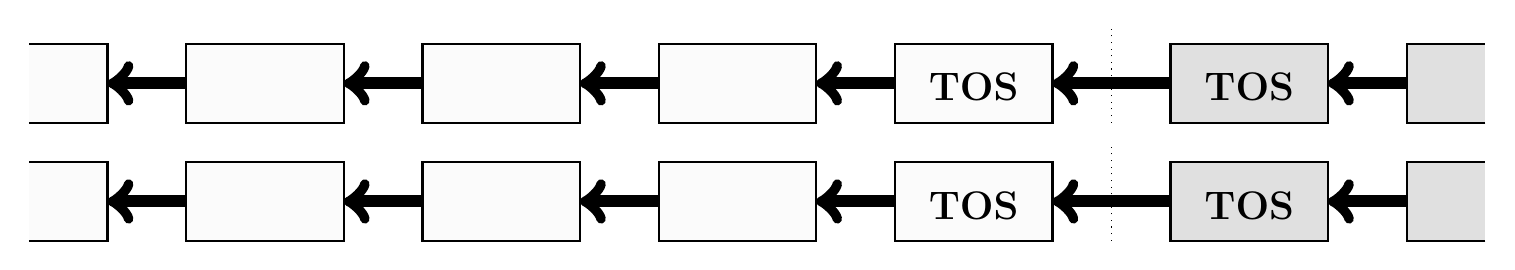
\begin{tikzpicture}

        \draw [thick, fill=gray!3]  (0,1.5) -- (1,1.5) -- (1,2.5) -- (0,2.5);%
        \draw [line width=1ex, <-]  (1,2)   -- (2,2);                %
        \draw [thick, fill=gray!3]  (2,1.5) rectangle (4,2.5);       %PS+3
        \draw [line width=1ex, <-]  (4,2)   -- (5,2);                %
        \draw [thick, fill=gray!3]  (5,1.5) rectangle (7,2.5);       %PS+2
        \draw [line width=1ex, <-]  (7,2)   -- (8,2);                %
        \draw [thick, fill=gray!3]  (8,1.5) rectangle (10,2.5);      %PS+1
        \draw [line width=1ex, <-]  (10,2)  -- (11,2);               %
        \draw [thick, fill=gray!3]  (11,1.5) rectangle (13,2.5);     %PS TOS
        \node at (12,1.95)          {\Large{\textbf{TOS}}};          %
        \draw [line width=1ex, <-]  (13,2)  -- (14.5,2);             %
        \draw [dotted]              (13.75,1.5) -- (13.75,2.7);      %
        \draw [thick, fill=gray!24] (14.5,1.5) rectangle (16.5,2.5); %RS TOS
        \node at (15.5,1.95)        {\Large{\textbf{TOS}}};          %
        \draw [line width=1ex, <-]  (16.5,2) -- (17.5,2);            % 
        \draw [thick, fill=gray!24] (18.5,1.5) -- (17.5,1.5) -- (17.5,2.5) -- (18.5,2.5);

        \draw [thick, fill=gray!3]  (0,0) -- (1,0) -- (1,1) -- (0,1);%
        \draw [line width=1ex, <-]  (1,0.5) -- (2,0.5);              %
        \draw [thick, fill=gray!3]  (2,0) rectangle (4,1);           %PS+3
        \draw [line width=1ex, <-]  (4,0.5) -- (5,0.5);              %
        \draw [thick, fill=gray!3]  (5,0) rectangle (7,1);           %PS+2
        \draw [line width=1ex, <-]  (7,0.5) -- (8,0.5);              %
        \draw [thick, fill=gray!3]  (8,0) rectangle (10,1);          %PS+1
        \draw [line width=1ex, <-]  (10,0.5) -- (11,0.5);            %
        \draw [thick, fill=gray!3]  (11,0) rectangle (13,1);         %PS TOS
        \node at (12,0.45)          {\Large{\textbf{TOS}}};          %
        \draw [line width=1ex, <-]  (13,0.5)  -- (14.5,0.5);         %
        \draw [dotted]              (13.75,0) -- (13.75,1.2);        %
        \draw [thick, fill=gray!24] (14.5,0) rectangle (16.5,1);     %RS TOS
        \node at (15.5,0.45)        {\Large{\textbf{TOS}}};          %
        \draw [line width=1ex, <-]  (16.5,0.5) -- (17.5,0.5);        % 
        \draw [thick, fill=gray!24] (18.5,0) -- (17.5,0) -- (17.5,1) -- (18.5,1);
      \end{tikzpicture}
    }} &
    \multicolumn{1}{m{4.25em}|}{
    \makecell[c]{ 
      \texttt{0x0755} \\ 
      \texttt{0x0755}
    }} \\ \hline
  \end{longtable}
\end{center}  
\endgroup

\subsubsection{Stack Underflow Detection}
\label{opcodes:stack:uf}

The required number of arguments for a stack instruction is determined by the transition pattern
(\gls{ust} and \gls{ist} fields).
The rules listed in \tabref{opcodes:stack:ufrules} are applied.


subsubsection{Common Stack Operations}
\label{opcodes:stack:ops}
\tabref{opcodes:stack:mapping} shows how common \gls{stack} operations in \gls{forth} are mapped N1 instructions. 

\begingroup
\setlength{\LTleft}{-20cm plus -1fill}
\setlength{\LTright}{\LTleft}
\begin{center}
  \rowcolors{1}{gray!12}{white}                                         %set alternating row color
  \begin{longtable}{|c|c|c|}
    \rowcolor{white}
    \caption{Rules of Stack Underflow Detection}
    \label{opcodes:stack:ufrules} \\
    %Header
    \hline                                     
    \rowcolor{gray!25}
    \multicolumn{1}{|c|}{\textbf{\rule{0pt}{2.5ex}Rule}}       &  
    \multicolumn{1}{c|}{\textbf{\rule{0pt}{2.5ex}Transitions}} & 
    \multicolumn{1}{c|}{\textbf{\rule{0pt}{2.5ex}Description}} \\
    \hline
    \endhead                               
    %Footers
    \hline
    \rowcolor{white}
    \multicolumn{3}{r}{\tiny{...continued}} \\
    \endfoot
    \hline
    \endlastfoot

    %DROP rule
    \multicolumn{1}{|m{3em}|}{
    \makecell[c]{ 
      ``\texttt{DROP}''\\
      Rule}} &
    \multicolumn{1}{m{7em}|}{
    \scalebox{0.4} {
      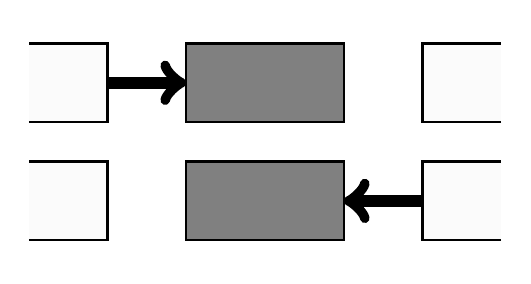
\begin{tikzpicture}
        \path []  (0,-0.2)   -- (0,2.7);       
        
        \draw [thick, fill=gray!3]  (0,1.5) -- (1,1.5) -- (1,2.5) -- (0,2.5);
        \draw [line width=1ex, ->]  (1,2)   -- (2,2);                        
        \draw [thick, fill=gray]    (2,1.5) rectangle (4,2.5);              
        \draw [thick, fill=gray!3]  (6,1.5) -- (5,1.5) -- (5,2.5) -- (6,2.5);

        \draw [thick, fill=gray!3]  (0,0) -- (1,0) -- (1,1) -- (0,1);        
        \draw [thick, fill=gray]    (2,0) rectangle (4,1);                   
        \draw [line width=1ex, <-]  (4,0.5) -- (5,0.5);                      
        \draw [thick, fill=gray!3]  (6,0) -- (5,0) -- (5,1) -- (6,1);
      \end{tikzpicture}
    }} &
    %\multicolumn{1}{m{32em}|}{
    \makecell[l]{
    \begin{minipage}[t]{\linewidth}%  
      A cell that will be dropped (overwritten, without passing on it's content)
      from either direction must hold content, otherwise a stack underflow exception
      will be triggered.
    \end{minipage}%
   } \\ \hline

    %DUP rule
    \multicolumn{1}{|m{3em}|}{
    \makecell[c]{ 
      ``\texttt{DUP}''\\
      Rule}} &
    \multicolumn{1}{m{7em}|}{
    \scalebox{0.4} {
      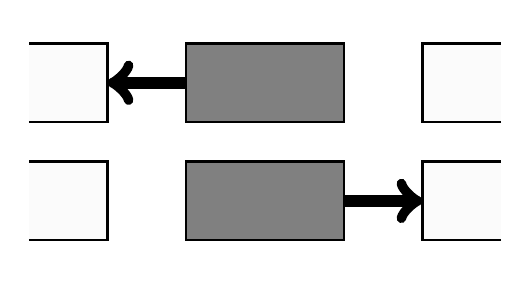
\begin{tikzpicture}
        \path []  (0,-0.2)   -- (0,2.7);       
        
        \draw [thick, fill=gray!3]  (0,1.5) -- (1,1.5) -- (1,2.5) -- (0,2.5);
        \draw [line width=1ex, <-]  (1,2)   -- (2,2);                        
        \draw [thick, fill=gray]    (2,1.5) rectangle (4,2.5);              
        \draw [thick, fill=gray!3]  (6,1.5) -- (5,1.5) -- (5,2.5) -- (6,2.5);

        \draw [thick, fill=gray!3]  (0,0) -- (1,0) -- (1,1) -- (0,1);        
        \draw [thick, fill=gray]    (2,0) rectangle (4,1);                   
        \draw [line width=1ex, ->]  (4,0.5) -- (5,0.5);                      
        \draw [thick, fill=gray!3]  (6,0) -- (5,0) -- (5,1) -- (6,1);
      \end{tikzpicture}
    }} &
    %\multicolumn{1}{m{32em}|}{
    \makecell[l]{ 
    \begin{minipage}[t]{\linewidth}%  
      A cell that will be duplicated in either direction must hold content,
      otherwise a stack underflow exception will be triggered.
    \end{minipage}%
    } \\ \hline

    %SWAP rule
    \multicolumn{1}{|m{3em}|}{
    \makecell[c]{ 
      ``\texttt{SWAP}''\\
      Rule}} &
    \multicolumn{1}{m{7em}|}{
    \scalebox{0.4} {
      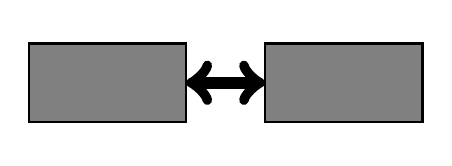
\begin{tikzpicture}
        \path []  (2.25,1.3)   -- (2.25,2.7);       
        
        \draw [thick, fill=gray]     (2.25,1.5) rectangle (4.25,2.5); 
        \draw [line width=1ex, <->]  (4.25,2)   -- (5.25,2);          
        \draw [thick, fill=gray]     (5.25,1.5) rectangle (7.25,2.5); 
      \end{tikzpicture}
    }} &
    %\multicolumn{1}{m{32em}|}{
    \makecell[l]{ 
    \begin{minipage}[t]{\linewidth}%  
      Two neighboring cells that will be swapped must both hold content,
      otherwise a stack underflow exception will be triggered.
    \end{minipage}%
    } \\ \hline

    %Shift rule
    \multicolumn{1}{|m{3em}|}{
    \makecell[c]{ 
      ``Shift''\\
      Rule}} &
    \multicolumn{1}{m{7em}|}{
    \scalebox{0.4} {
      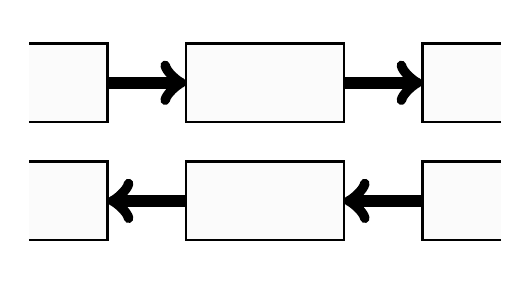
\begin{tikzpicture}
        \path []  (0,-0.2)   -- (0,2.7);       
        
        \draw [thick, fill=gray!3]  (0,1.5) -- (1,1.5) -- (1,2.5) -- (0,2.5);
        \draw [line width=1ex, ->]  (1,2)   -- (2,2);                        
        \draw [thick, fill=gray!3]  (2,1.5) rectangle (4,2.5);              
        \draw [line width=1ex, ->]  (4,2) -- (5,2);                      
        \draw [thick, fill=gray!3]  (6,1.5) -- (5,1.5) -- (5,2.5) -- (6,2.5);

        \draw [thick, fill=gray!3]  (0,0) -- (1,0) -- (1,1) -- (0,1);        
        \draw [line width=1ex, <-]  (1,0.5)   -- (2,0.5);                        
        \draw [thick, fill=gray!3]  (2,0) rectangle (4,1);                   
        \draw [line width=1ex, <-]  (4,0.5) -- (5,0.5);                      
        \draw [thick, fill=gray!3]  (6,0) -- (5,0) -- (5,1) -- (6,1);
      \end{tikzpicture}
    }} &
    %\multicolumn{1}{m{32em}|}{
    \makecell[l]{ 
    \begin{minipage}[t]{\linewidth}%  
      Cells that will be shifted in either direction, will not be checked for content
    \end{minipage}%
    } \\ \hline

    %Cross rule
    \multicolumn{1}{|m{3em}|}{
    \makecell[c]{ 
      ``Cross''\\
      Rule}} &
    \multicolumn{1}{m{7em}|}{
    \scalebox{0.4} {
      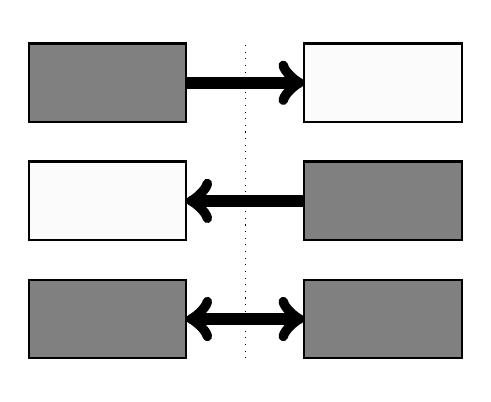
\begin{tikzpicture}

       \path []                      (2,-0.2) --  (2,4.2);             
       \draw [dotted]                (4.75,0) --  (4.75,4);

        \draw [thick, fill=gray]     (2,3) rectangle (4,4); 
        \draw [line width=1ex, ->]   (4,3.5)   -- (5.5,3.5);          
        \draw [thick, fill=gray!3]   (5.5,3) rectangle (7.5,4); 

        \draw [thick, fill=gray!3]   (2,1.5) rectangle (4,2.5); 
        \draw [line width=1ex, <-]   (4,2)   -- (5.5,2);          
        \draw [thick, fill=gray]     (5.5,1.5) rectangle (7.5,2.5); 

        \draw [thick, fill=gray]     (2,0) rectangle (4,1); 
        \draw [line width=1ex, <->]  (4,0.5)   -- (5.5,0.5);          
        \draw [thick, fill=gray]     (5.5,0) rectangle (7.5,1); 

     \end{tikzpicture}
    }} &
    %\multicolumn{1}{m{32em}|}{
    \makecell[l]{ 
    \begin{minipage}[t]{\linewidth}%  
      Any cell that is shifted, swapped or duplicated across the \gls{ps}/\gls{rs} boundary
      must hold content, otherwise a stack underflow exception will be triggered.
    \end{minipage}%
    } \\ \hline

  \end{longtable}
\end{center}  
\endgroup

%Memory Access Instructions
\subsection{Memory Access Instructions}
\label{opcodes:memacc}

Memory access instruction perform read or write acesses to the system's 64K word (128KB) address space.
Data is solely accessed in 16-bit entities.
Accesses to a 255 word (510B) window in the main address space, can be done through an immediate
addressing. This offers faster access to frequently used system variables.

%Function Register access
\subsection{Function Register Access}
\label{opcodes:freg}

The N1 processor provides a set \glspl{freg}, which provide access to a number of processor features
(see \tabref{opcodes:freg:tab}).
These \glspl{freg} are read and written through special \glspl{opcode}.

\begingroup
\setlength{\LTleft}{-20cm plus -1fill}
\setlength{\LTright}{\LTleft}
\begin{center}
  \rowcolors{1}{gray!12}{white}                                         %set alternating row color
  \begin{longtable}{|c|c|c|}
    \rowcolor{white}
    \caption{\Glspl{freg}}
    \label{opcodes:freg:tab} \\
    %Header
    \hline                                     
    \rowcolor{gray!25}
    \multicolumn{1}{|c|}{\textbf{\rule{0pt}{2.5ex}Address}} &  
    \multicolumn{1}{c|}{\textbf{\rule{0pt}{2.5ex}Mnemonic}} &
    \multicolumn{1}{c|}{\textbf{\rule{0pt}{2.5ex}Name}}     \\
    \hline
    \endhead                               
    %Footers
    \hline
    \rowcolor{white}
    \multicolumn{3}{r}{\tiny{...continued}} \\
    \endfoot
    \hline
    \endlastfoot

    %%Carry register (CRY)
    %\texttt{0x00}                               &
    %\hyperref[opcodes:freg:cry]{CRY}            &
    %\hyperref[opcodes:freg:cry]{Carry Register} \\ \hline

    %Parameter Stack Depth Register (PSD)
    \texttt{0x00}                                               &
    \hyperref[opcodes:freg:psd]{PSD}                            &
    \hyperref[opcodes:freg:psd]{Parameter Stack Depth Register} \\ \hline

    %Return Stack Depth Register (PSD)
    \texttt{0x01}                                            &
    \hyperref[opcodes:freg:psd]{RSD}                         &
    \hyperref[opcodes:freg:psd]{Return Stack Depth Register} \\ \hline
    
    %Exception and Interrupt Mask Register (EIM)
    \texttt{0x02}                                                      &
    \hyperref[opcodes:freg:eim]{EIM}                                   &
    \hyperref[opcodes:freg:eim]{Exception and Interrupt Mask Register} \\ \hline

  \end{longtable}
\end{center}  
\endgroup

%%Carry register (CRY)
%\subsubsection{Carry Register (CRY)}
%\label{opcodes:freg:cry}
%
%\begin{figure}[H]
%  %\begin{center}
%  \makebox[\textwidth][c]{
%    %\scalebox{0.5125} {
%    \scalebox{0.515} {
%      \begin{tikzpicture}
%
%        %Offset
%        \node [align=left, anchor=west] at (-2,3) {
%          \huge{Offset: \texttt{0x00}}
%        };        
%        %Index
%        \node [above] at  (1,2) {15};
%        \node [above] at  (3,2) {14};
%        \node [above] at  (5,2) {13};
%        \node [above] at  (7,2) {12};
%        \node [above] at  (9,2) {11};
%        \node [above] at (11,2) {10};
%        \node [above] at (13,2) {9};
%        \node [above] at (15,2) {8};
%        \node [above] at (17,2) {7};
%        \node [above] at (19,2) {6};
%        \node [above] at (21,2) {5};
%        \node [above] at (23,2) {4};
%        \node [above] at (25,2) {3};
%        \node [above] at (27,2) {2};
%        \node [above] at (29,2) {1};
%        \node [above] at (31,2) {0};
%        %Read
%        \node [align=right, anchor=east] at (0,1.5) {\large{Read}};
%        %\draw [thick, fill=white]  (0,1) rectangle (32,2);
%        \draw [thick, fill=gray!3]  (0,1) rectangle  (32,2); %15..0
%        \node at (15,1.5) {\huge{\texttt{CRY}}};
%        %Write
%        \node [align=right, anchor=east] at (0,0.5) {\large{Write}};
%        \draw [thick, fill=white]  (0,0) rectangle (32,1);
%        %\draw [thick, fill=gray!3]  (0,0) rectangle  (32,2); %15..0
%        %\node at (15,0.5) {\huge{\texttt{CRY}}};
%      \end{tikzpicture}
%    }
%  }
%  %\caption{Carry Register}
%  %\label{opcodes:freg:cry:fig}
%  %\end{center}
%\end{figure}
%
%The Carry Register captures the carry or borrow flag of the last addition or suntraction.
%It alwyayread one of the three values:
%\begin{itemize}
%  \item \texttt{1} (carry from the last addition
%  \item \texttt{0} (no carry or borrow)
%  \item \texttt{-1} (borrow from the last subtraction)
%\end{itemize}
%
%\begingroup
%\setlength{\LTleft}{-20cm plus -1fill}
%\setlength{\LTright}{\LTleft}
%\begin{center}
%  \rowcolors{1}{gray!12}{white}                                         %set alternating row color
%  \begin{longtable}{|c|c|c|c|}
%    \rowcolor{white}
%    \caption{Carry  Register Bit Description}
%    \label{opcodes:freg:cry:tab} \\
%    %Header
%    \hline                                     
%    \rowcolor{gray!25}
%    \multicolumn{1}{|c|}{\textbf{\rule{0pt}{2.5ex}Bit}}  &  
%    \multicolumn{1}{c|}{\textbf{\rule{0pt}{2.5ex}Postion}}    & 
%    \multicolumn{1}{c|}{\textbf{\rule{0pt}{2.5ex}Description}} \\
%     \hline
%    \endhead                               
%    %Footers
%    \hline
%    \rowcolor{white}
%    \multicolumn{4}{r}{\tiny{...continued}} \\
%    \endfoot
%    \hline
%    \endlastfoot
%
%    %CRY
%    \texttt{CRY} &
%    15..0        &
%    \multicolumn{1}{m{36em}|}{
%      \makecell[l]{
%        \begin{minipage}[t]{\linewidth}%  
%          \centerline{\textbf{Return Stack Depth}}
%          \begin{description}[style=nextline]
%          \item[Read:]
%            Carry or borrow from last addition or subtraction.\\[1pt]
%          \end{description}
%        \end{minipage}%
%    }}  \\ \hline
%
%  \end{longtable}
%\end{center}  
%\endgroup
%
%~\\

%Parameter Stack Depth Reggister (PSD)
\subsubsection{Parameter Stack Depth Register (PSD)}
\label{opcodes:freg:psd}

\begin{figure}[H]
  %\begin{center}
  \makebox[\textwidth][c]{
    %\scalebox{0.5125} {
    \scalebox{0.515} {
      \begin{tikzpicture}

        %Offset
        \node [align=left, anchor=west] at (-2,3) {
          \huge{Offset: \texttt{0x00}}
        };        
        %Index
        \node [above] at  (1,2) {15};
        \node [above] at  (3,2) {14};
        \node [above] at  (5,2) {13};
        \node [above] at  (7,2) {12};
        \node [above] at  (9,2) {11};
        \node [above] at (11,2) {10};
        \node [above] at (13,2) {9};
        \node [above] at (15,2) {8};
        \node [above] at (17,2) {7};
        \node [above] at (19,2) {6};
        \node [above] at (21,2) {5};
        \node [above] at (23,2) {4};
        \node [above] at (25,2) {3};
        \node [above] at (27,2) {2};
        \node [above] at (29,2) {1};
        \node [above] at (31,2) {0};
        %Read
        \node [align=right, anchor=east] at (0,1.5) {\large{Read}};
        %\draw [thick, fill=white]  (0,1) rectangle (32,2);
        \draw [thick, fill=gray!3]  (0,1) rectangle  (32,2); %15..0
        \node at (15,1.5) {\huge{\texttt{PSD}}};
        %Write
        \node [align=right, anchor=east] at (0,0.5) {\large{Write}};
        %\draw [thick, fill=white]  (0,0) rectangle (32,1);
        \draw [thick, fill=gray!3]  (0,0) rectangle  (32,1); %15..0
        \node at (15,0.5) {\huge{\texttt{PSDCLR}}};
      \end{tikzpicture}
    }
  }
  %\caption{Parameter Stack Depth Register}
  %\label{opcodes:freg:psd:fig}
  %\end{center}
\end{figure}

The current depth of the \gls{ps} is captured in the parameter stack depth register. \\
Writing \texttt{0x0000} to this register will clear the \gls{ps}.

\begingroup
\setlength{\LTleft}{-20cm plus -1fill}
\setlength{\LTright}{\LTleft}
\begin{center}
  \rowcolors{1}{gray!12}{white}                                         %set alternating row color
  \begin{longtable}{|c|c|c|c|}
    \rowcolor{white}
    \caption{Parameter Stack Depth Register Bit Description}
    \label{opcodes:freg:psd:tab} \\
    %Header
    \hline                                     
    \rowcolor{gray!25}
    \multicolumn{1}{|c|}{\textbf{\rule{0pt}{2.5ex}Bit}}  &  
    \multicolumn{1}{c|}{\textbf{\rule{0pt}{2.5ex}Postion}}    & 
    \multicolumn{1}{c|}{\textbf{\rule{0pt}{2.5ex}Description}} \\
     \hline
    \endhead                               
    %Footers
    \hline
    \rowcolor{white}
    \multicolumn{4}{r}{\tiny{...continued}} \\
    \endfoot
    \hline
    \endlastfoot

    %PSD
    \texttt{PSD} &
    15..0        &
    \multicolumn{1}{m{36em}|}{
      \makecell[l]{
        \begin{minipage}[t]{\linewidth}%  
          \centerline{\textbf{Parameter Stack Depth}}
          \begin{description}[style=nextline]
          \item[Read:]
            Current parameter stack depth\\[1pt]
          \end{description}
        \end{minipage}%
    }}  \\ \hline

    %PSDCLR
    \texttt{PSDCLR} &
    15..0        &
    \multicolumn{1}{m{36em}|}{
      \makecell[l]{
        \begin{minipage}[t]{\linewidth}%  
          \centerline{\textbf{Clear Parameter Stack}}
          \begin{description}[style=nextline]
          \item[Write:]
            Writing the value \texttt{0x0000} will clrear the \gls{ps}.\\
            All other write accesses have no effect.\\[1pt]
          \end{description}
        \end{minipage}%
    }}  \\ \hline
 
  \end{longtable}
\end{center}  
\endgroup

~\\

%Return Stack Depth Register (RSD)
\subsubsection{Return Stack Depth Register (RSD}
\label{opcodes:freg:rsd}

\begin{figure}[H]
  %\begin{center}
  \makebox[\textwidth][c]{
    %\scalebox{0.5125} {
    \scalebox{0.515} {
      \begin{tikzpicture}

        %Offset
        \node [align=left, anchor=west] at (-2,3) {
          \huge{Offset: \texttt{0x01}}
        };        
        %Index
        \node [above] at  (1,2) {15};
        \node [above] at  (3,2) {14};
        \node [above] at  (5,2) {13};
        \node [above] at  (7,2) {12};
        \node [above] at  (9,2) {11};
        \node [above] at (11,2) {10};
        \node [above] at (13,2) {9};
        \node [above] at (15,2) {8};
        \node [above] at (17,2) {7};
        \node [above] at (19,2) {6};
        \node [above] at (21,2) {5};
        \node [above] at (23,2) {4};
        \node [above] at (25,2) {3};
        \node [above] at (27,2) {2};
        \node [above] at (29,2) {1};
        \node [above] at (31,2) {0};
        %Read
        \node [align=right, anchor=east] at (0,1.5) {\large{Read}};
        %\draw [thick, fill=white]  (0,1) rectangle (32,2);
        \draw [thick, fill=gray!3]  (0,1) rectangle  (32,2); %15..0
        \node at (15,1.5) {\huge{\texttt{RSP}}};
        %Write
        \node [align=right, anchor=east] at (0,0.5) {\large{Write}};
        %\draw [thick, fill=white]  (0,0) rectangle (32,1);
        \draw [thick, fill=gray!3]  (0,0) rectangle  (32,1); %15..0
        \node at (15,0.5) {\huge{\texttt{RSPCLR}}};
      \end{tikzpicture}
    }
  }
  %\caption{Return Stack Depth Register}
  %\label{opcodes:freg:rsd:fig}
  %\end{center}
\end{figure}

The current depth of the \gls{rs} is captured in the parameter stack depth register. \\
Writing \texttt{0x0000} to this register will clear the \gls{rs}.

\begingroup
\setlength{\LTleft}{-20cm plus -1fill}
\setlength{\LTright}{\LTleft}
\begin{center}
  \rowcolors{1}{gray!12}{white}                                         %set alternating row color
  \begin{longtable}{|c|c|c|c|}
    \rowcolor{white}
    \caption{Return Stack Depth Register Bit Description}
    \label{opcodes:freg:rsd:tab} \\
    %Header
    \hline                                     
    \rowcolor{gray!25}
    \multicolumn{1}{|c|}{\textbf{\rule{0pt}{2.5ex}Bit}}  &  
    \multicolumn{1}{c|}{\textbf{\rule{0pt}{2.5ex}Postion}}    & 
    \multicolumn{1}{c|}{\textbf{\rule{0pt}{2.5ex}Description}} \\
     \hline
    \endhead                               
    %Footers
    \hline
    \rowcolor{white}
    \multicolumn{4}{r}{\tiny{...continued}} \\
    \endfoot
    \hline
    \endlastfoot

    %RSD
    \texttt{RSD} &
    15..0        &
    \multicolumn{1}{m{36em}|}{
      \makecell[l]{
        \begin{minipage}[t]{\linewidth}%  
          \centerline{\textbf{Return Stack Depth}}
          \begin{description}[style=nextline]
          \item[Read:]
            Current return stack depth.\\[1pt]
          \end{description}
        \end{minipage}%
    }}  \\ \hline

    %RSDCLR
    \texttt{RSDCLR} &
    15..0        &
    \multicolumn{1}{m{36em}|}{
      \makecell[l]{
        \begin{minipage}[t]{\linewidth}%  
          \centerline{\textbf{Return Stack Depth}}
          \begin{description}[style=nextline]
          \item[Write:]
            Writing the value \texttt{0x0000} will clrear the \gls{rs}.\\
            All other write accesses have no effect.\\[1pt]
          \end{description}
        \end{minipage}%
    }}  \\ \hline

  \end{longtable}
\end{center}  
\endgroup

~\\

%Exception and Interrupt Mask Register (EIM)
\subsubsection{Exception and Interrupt Mask Register (EIM)}
\label{opcodes:freg:eim}

\begin{figure}[H]
  %\begin{center}
  \makebox[\textwidth][c]{
    %\scalebox{0.5125} {
    \scalebox{0.515} {
      \begin{tikzpicture}

        %Offset
        \node [align=left, anchor=west] at (-2,3) {
          \huge{Offset: \texttt{0x02}}
        };        
        %Index
        \node [above] at  (1,2) {15};
        \node [above] at  (3,2) {14};
        \node [above] at  (5,2) {13};
        \node [above] at  (7,2) {12};
        \node [above] at  (9,2) {11};
        \node [above] at (11,2) {10};
        \node [above] at (13,2)  {9};
        \node [above] at (15,2)  {8};
        \node [above] at (17,2)  {7};
        \node [above] at (19,2)  {6};
        \node [above] at (21,2)  {5};
        \node [above] at (23,2)  {4};
        \node [above] at (25,2)  {3};
        \node [above] at (27,2)  {2};
        \node [above] at (29,2)  {1};
        \node [above] at (31,2)  {0};
        %Read
        \node [align=right, anchor=east] at (0,1.5) {\large{Read}};
        \draw [thick, fill=white] (0,1) rectangle (32,2);
        \node at ( 1,1.5) {\huge{\texttt{0}}};               %15
        \node at ( 3,1.5) {\huge{\texttt{0}}};               %14
        \node at ( 5,1.5) {\huge{\texttt{0}}};               %13
        \node at ( 7,1.5) {\huge{\texttt{0}}};               %12
        \node at ( 9,1.5) {\huge{\texttt{0}}};               %11
        \node at (11,1.5) {\huge{\texttt{0}}};               %10
        \node at (13,1.5) {\huge{\texttt{0}}};               % 9
        \node at (15,1.5) {\huge{\texttt{0}}};               % 8
        \node at (17,1.5) {\huge{\texttt{0}}};               % 7
        \node at (19,1.5) {\huge{\texttt{0}}};               % 6
        \node at (21,1.5) {\huge{\texttt{0}}};               % 5
        \node at (23,1.5) {\huge{\texttt{0}}};               % 4
        \node at (25,1.5) {\huge{\texttt{0}}};               % 3
        \node at (29,1.5) {\huge{\texttt{0}}};               % 1
        %Write
        \node [align=right, anchor=east] at (0,0.5) {\large{Write}};
        \draw [thick, fill=white] (0,0) rectangle (32,1);
        \draw [thick, fill=gray!3] (24,0) rectangle (26,1);  % 3
        \node at (25,0.5) {\Large{\texttt{EMWE}}};
        \draw [thick, fill=gray!3] (26,0) rectangle (28,2);  % 2
        \node at (27,1)   {\Large{\texttt{EM}}};
        \draw [thick, fill=gray!3] (28,0) rectangle (30,1);  % 1
        \node at (29,0.5) {\Large{\texttt{IMWE}}};
        \draw [thick, fill=gray!3] (30,0) rectangle (32,2);  % 0
        \node at (31,1)   {\Large{\texttt{IM}}};
        \end{tikzpicture}
    }
  }
  %\caption{Interrupt and Exception Enable Register}
  %\label{opcodes:freg:eim:fig}
  %\end{center}
\end{figure}

Interrupt and exception handling can be disabled through two control register bits:
\texttt{IM} (interrupt mask) and \texttt{EM} (exception mask).
This is to avoid \gls{rs} overflows, caused by nested execution of exceptions and interrupt sevice routines.

The \texttt{IM} bit is automatically set when an interrupt service routine is started.
The \texttt{eM} bit is automatically set when an exception handler is executed.
Both flags mut be set manually as soon as new interrupts or exceptions can be processed.
Each one of these bits is protected by a write enable bit to atomic bit manipulations.

\begingroup
\setlength{\LTleft}{-20cm plus -1fill}
\setlength{\LTright}{\LTleft}
\begin{center}
  \rowcolors{1}{gray!12}{white}                                         %set alternating row color
  \begin{longtable}{|c|c|c|c|}
    \rowcolor{white}
    \caption{Exception and Interrupt Mask Register Bit Description}
    \label{opcodes:freg:eim:tab} \\
    %Header
    \hline                                     
    \rowcolor{gray!25}
    \multicolumn{1}{|c|}{\textbf{\rule{0pt}{2.5ex}Bit}}       &  
    \multicolumn{1}{c|}{\textbf{\rule{0pt}{2.5ex}Postion}}    & 
    \multicolumn{1}{c|}{\textbf{\rule{0pt}{2.5ex}Description}} \\
     \hline
    \endhead                               
    %Footers
    \hline
    \rowcolor{white}
    \multicolumn{4}{r}{\tiny{...continued}} \\
    \endfoot
    \hline
    \endlastfoot

    %EMWE
    \texttt{EMWE} &
    3               &
    \multicolumn{1}{m{36em}|}{
      \makecell[l]{
        \begin{minipage}[t]{\linewidth}%  
          \centerline{\textbf{Exception Mask Write Enable}}
          \begin{description}[style=nextline]
          %\item[Read:]
          %  Always reads zero.
          \item[Write:]
            Writing a \texttt{1} allows modification of the \texttt{EM} bit in the same access.\\[1pt]
          \end{description}
        \end{minipage}%
    }}  \\ \hline
    
   %EM
   \texttt{EM} &
   2               &
   \multicolumn{1}{m{36em}|}{
   \makecell[l]{ 
     \begin{minipage}[t]{\linewidth}%  
     \centerline{\textbf{Exception Mask}}
     \begin{description}[style=nextline]
     \item[Read:]
     \begin{minipage}[t]{\linewidth}  
       \begin{description}[style=multiline]
         \item[\texttt{0}:]
           Exceptions are enabled.
         \item[\texttt{1}:]
           Exceptions are disbled.
         \end{description}
     \end{minipage}
     \item[Write:]
     \begin{minipage}[t]{\linewidth}
       \begin{description}[style=multiline]
         \item[\texttt{0}:]
            Disable exceptions. Only possible while instantly writing a \texttt{1} to \texttt{EMWE}. 
         \item[\texttt{1}:]
           Disable exceptions. Only possible while instantly writing a \texttt{1} to \texttt{EMWE}.\\[1pt]
       \end{description}
     \end{minipage}  
     \end{description}
     \end{minipage}%
   }}  \\ \hline
   
    %IMWE
    \texttt{IMWE} &
    1               &
    \multicolumn{1}{m{36em}|}{
      \makecell[l]{
        \begin{minipage}[t]{\linewidth}%  
          \centerline{\textbf{Interrupt Mask Write Enable}}
          \begin{description}[style=nextline]
          %\item[Read:]
          %  Always reads zero.
          \item[Write:]
            Writing a \texttt{1} allows modification of the \texttt{IM} bit in the same access.\\[1pt]
          \end{description}
        \end{minipage}%
    }}  \\ \hline
    
   %IM
   \texttt{IEN} &
   0               &
   \multicolumn{1}{m{36em}|}{
   \makecell[l]{ 
     \begin{minipage}[t]{\linewidth}%  
     \centerline{\textbf{Interrupt Mask}}
     \begin{description}[style=nextline]
     \item[Read:]
     \begin{minipage}[t]{\linewidth}  
       \begin{description}[style=multiline]
         \item[\texttt{0}:]
           Interrupts are enabled.
         \item[\texttt{1}:]
           Interrupts are disabled.
         \end{description}
     \end{minipage}
     \item[Write:]
     \begin{minipage}[t]{\linewidth}
       \begin{description}[style=multiline]
         \item[\texttt{0}:]
            Disable interrupts. Only possible while instantly writing a \texttt{1} to \texttt{IMWE}. 
         \item[\texttt{1}:]
           Disable interrupts. Only possible while instantly writing a \texttt{1} to \texttt{IMWE}.\\[1pt]
       \end{description}
     \end{minipage}  
     \end{description}
     \end{minipage}%
   }}  \\ \hline
   
  \end{longtable}
\end{center}  
\endgroup



%--------------------
% ANS Forth core words
%--------------------
%###############################################################################
%# N1 - Manual - ANS Forth words                                               #
%###############################################################################
%#    Copyright 2018 - 2019 Dirk Heisswolf                                     #
%#    This file is part of the N1 project.                                     #
%#                                                                             #
%#    N1 is free software: you can redistribute it and/or modify               #
%#    it under the terms of the GNU General Public License as published by     #
%#    the Free Software Foundation, either version 3 of the License, or        #
%#    (at your option) any later version.                                      #
%#                                                                             #
%#    N1 is distributed in the hope that it will be useful,                    #
%#    but WITHOUT ANY WARRANTY; without even the implied warranty of           #
%#    MERCHANTABILITY or FITNESS FOR A PARTICULAR PURPOSE.  See the            #
%#    GNU General Public License for more details.                             #
%#                                                                             #
%#    You should have received a copy of the GNU General Public License        #
%#    along with N1.  If not, see <http://www.gnu.org/licenses/>.              #
%###############################################################################
%# Version History:                                                            #
%#   January 3, 2019                                                           #
%#      - Initial release                                                      #
%###############################################################################

\section{ANS Forth Words}
\label{N1_words}

The N1 processor aims at executing Forth code in an efficient way.
\tabref{words:list} provides a list of standard ANS Forth\cite{dpans94} words 
which can be easily mapped to N1 instructions. 

\begingroup
\setlength{\LTleft}{-20cm plus -1fill}
\setlength{\LTright}{\LTleft}
\begin{center}
  \rowcolors{1}{gray!12}{white}                                         %set alternating row color
  \begin{longtable}{|c|c|l|c|}
    \rowcolor{white}
    \caption{ANS Forth words}
    \label{words:list} \\
    %Header
    \hline                                     
    \rowcolor{gray!25}
    \multicolumn{1}{|c|}{\textbf{\rule{0pt}{2.5ex}Word}}          &  
    \multicolumn{1}{c|}{\textbf{\rule{0pt}{2.5ex}Stack}}          &
    \multicolumn{1}{c|}{\textbf{\rule{0pt}{2.5ex}Description}}    &
    \multicolumn{1}{c|}{\textbf{\rule{0pt}{2.5ex}Opcode}} \\
    \hline
    \endhead                               
    %Footers
    \hline
    \rowcolor{white}
    \multicolumn{4}{r}{\tiny{...continued}} \\
    \endfoot
    \hline
    \endlastfoot
    
    %! 
      \texttt{!}                                                  &
      ( x addr -- )                                               &
      \multicolumn{1}{m{36ex}|}{
        \makecell[l]{                   
          Store x at addr}}                                       &
      \multicolumn{1}{m{9ex}|}{
        \makecell[c]{                   
          \texttt{0x02FF}}}                                       \\ \hline
                                              
    %*                                        
      \texttt{*}                                                  &
      ( n1$\mid$u1 n2$\mid$u2 -- n3$\mid$u3 )                     &
      \multicolumn{1}{m{36ex}|}{
        \makecell[l]{                   
          Multiply n1$\mid$u1 by n2$\mid$u2}}                     &
      \multicolumn{1}{m{9ex}|}{
        \makecell[c]{                   
          \texttt{0x0E00}}}                                       \\ \hline

    %+                                        
      \texttt{+}                                                  &
      ( n1$\mid$u1 n2$\mid$u2 -- n3$\mid$u3 )                     &
      \multicolumn{1}{m{36ex}|}{
        \makecell[l]{                   
          Add n1$\mid$u1 to n2$\mid$u2}}                          &
      \multicolumn{1}{m{9ex}|}{
        \makecell[c]{                   
          \texttt{0x0C00}}}                                       \\ \hline
                                              
    %+!                                        
      \texttt{+!}                                                 &
      ( n1$\mid$u1 a-adr -- )                                     &
      \multicolumn{1}{m{36ex}|}{
        \makecell[l]{                   
          Add n1$\mid$u1 to the cell at addr}}                    &
      \multicolumn{1}{m{9ex}|}{
        \makecell[c]{                   
          \texttt{0x0403}                                         \\        %copy addr to RS0 
          \texttt{0x03FF}                                         \\        %@
          \texttt{0x0C00}                                         \\        %+
          \texttt{0x0755}                                         \\        %R>
          \texttt{0x02FF}}}                                       \\ \hline %!
                                              
    %-                                        
      \texttt{-}                                                  &
      ( n1$\mid$u1 n2$\mid$u2 -- n3$\mid$u3 )                     &
      \multicolumn{1}{m{36ex}|}{
        \makecell[l]{                   
          Subtract n2$\mid$u2 from n1$\mid$u1}}                   &
      \multicolumn{1}{m{9ex}|}{
        \makecell[c]{                   
          \texttt{0x0C40}}}                                       \\ \hline
                              
    %0<                                        
      \texttt{0<}                                                 &
      ( n -- flag )                                               &
      \multicolumn{1}{m{36ex}|}{
        \makecell[l]{                   
          Test if n is negative}}                                 &
      \multicolumn{1}{m{9ex}|}{
        \makecell[c]{                   
          \texttt{0x0CF0}}}                                       \\ \hline
                              
    %0<>                                        
      \texttt{0<>}                                                &
      ( x -- flag )                                               &
      \multicolumn{1}{m{36ex}|}{
        \makecell[l]{                   
          Test if x is not zero}}                                 &
      \multicolumn{1}{m{9ex}|}{
        \makecell[c]{                   
          \texttt{0x0D70}}}                                       \\ \hline
                              
    %0>                                        
      \texttt{0>}                                                 &
      ( n -- flag )                                               &
      \multicolumn{1}{m{36ex}|}{
        \makecell[l]{                   
          Test if n is greater than zero}}                        &
      \multicolumn{1}{m{9ex}|}{
        \makecell[c]{                   
          \texttt{0x0CA0}}}                                       \\ \hline
                             
     %0=                                        
      \texttt{0=}                                                 &
      ( x -- flag )                                               &
      \multicolumn{1}{m{36ex}|}{
        \makecell[l]{                   
          Test if x is not zero}}                                 &
      \multicolumn{1}{m{9ex}|}{
        \makecell[c]{                   
          \texttt{0x0D70}}}                                       \\ \hline
                              
     %1+                                        
      \texttt{1+}                                                 &
      ( n1$\mid$u1 -- n2$\mid$u2 )                                &
      \multicolumn{1}{m{36ex}|}{
        \makecell[l]{                   
          Increment n1$\mid$u1}}                                  &
      \multicolumn{1}{m{9ex}|}{
        \makecell[c]{                   
          \texttt{0x0C01}}}                                       \\ \hline

     %1-                                        
      \texttt{1-}                                                 &
      ( n1$\mid$u1 -- n2$\mid$u2 )                                &
      \multicolumn{1}{m{36ex}|}{
        \makecell[l]{                   
          Decrement n1$\mid$u1}}                                  &
      \multicolumn{1}{m{9ex}|}{
        \makecell[c]{                   
          \texttt{0x0C1F}}}                                       \\ \hline

      %2!                                        
      \texttt{2!}                                                 &
      ( x1 x2 addr --  )                                          &
      \multicolumn{1}{m{36ex}|}{
        \makecell[l]{                   
          Store x2 at addr and x1 at addr+1}}                     &
      \multicolumn{1}{m{9ex}|}{
        \makecell[c]{                   
          \texttt{0x0750}                                         \\        %TUCK 
          \texttt{0x0460}                                         \\        % 
          \texttt{0x02FF}                                         \\        %!
          \texttt{0x0C01}                                         \\        %1+
          \texttt{0x02FF}}}                                       \\ \hline %!

     %2*                                        
      \texttt{2*}                                                 &
      ( x1 -- x2 )                                                &
      \multicolumn{1}{m{36ex}|}{
        \makecell[l]{                   
          Shift x1 one bit towards the \gls{msb}}}                &
      \multicolumn{1}{m{9ex}|}{
        \makecell[c]{                   
          \texttt{0x0F41}}}                                       \\ \hline

     %2/                                        
      \texttt{2/}                                                 &
      ( x1 -- x2 )                                                &
      \multicolumn{1}{m{36ex}|}{
        \makecell[l]{                   
          Shift x1 one bit towards the \gls{lsb},                 \\
          while the \gls{msb} remains unchanged}}                 &
      \multicolumn{1}{m{9ex}|}{
        \makecell[c]{                   
          \texttt{0x0F41}}}                                       \\ \hline

     %2@                                        
      \texttt{2@}                                                 &
      ( addr -- x1 x2 )                                           &
      \multicolumn{1}{m{36ex}|}{
        \makecell[l]{                   
          Fetch x2 from addr and x1 at                            \\
          addr+1}}                                                &
      \multicolumn{1}{m{9ex}|}{
        \makecell[c]{                   
          \texttt{0x0750}                                         \\        %DUP 
          \texttt{0x0C01}                                         \\        %1+ 
          \texttt{0x03FF}                                         \\        %@
          \texttt{0x0418}                                         \\        %SWAP
          \texttt{0x03FF}}}                                       \\ \hline %@

     %2DROP                                        
      \texttt{2DROP}                                              &
      ( x1 x2 -- )                                                &
      \multicolumn{1}{m{36ex}|}{
        \makecell[l]{                   
          Drop cell pair x1 x2 }}                                 &
      \multicolumn{1}{m{9ex}|}{
        \makecell[c]{                   
          \texttt{0x06A8}                                         \\        %DROP
          \texttt{0x06A8}}}                                       \\ \hline %DROP

     %2DUP                                       
      \texttt{2DUP}                                               &
      ( x1 x2 -- x1 x2 x1 x2 )                                    &
      \multicolumn{1}{m{36ex}|}{
        \makecell[l]{                   
          Drop cell pair x1 x2 }}                                 &
      \multicolumn{1}{m{9ex}|}{
        \makecell[c]{                   
          \texttt{0x0758}                                         \\        %SWAP and duplicate PS1
          \texttt{0x0758}}}                                       \\ \hline %SWAP and duplicate PS1

     %2OVER                                       
      \texttt{2OVER}                                              &
      ( x1 x2 x3 x4 -- x1 x2 x1 x2 x3 x4 x1 x2 )                  &
      \multicolumn{1}{m{36ex}|}{
        \makecell[l]{                   
          Copy cell pair x1 x2 to the \gls{tos}}}                 &
      \multicolumn{1}{m{9ex}|}{
        \makecell[c]{                   
          \texttt{0x0750}                                         \\        %PS4<-PS3<>PS2  PS1  PS0
          \texttt{0x0460}                                         \\        %PS4  PS3  PS2<>PS1  PS0
          \texttt{0x0789}                                         \\        %PS4<-PS3<>PS2  PS1<>PS0
          \texttt{0x0460}}}                                       \\ \hline %PS4  PS3  PS2<>PS1  PS0

     %2>R                                        
      \texttt{2>R}                                                &
       ( x1 x2 -- ) (R: -- x1 x2 )                                &
      \multicolumn{1}{m{36ex}|}{
        \makecell[l]{                   
          Shift cell pair x1 x2 to the                            \\
          \gls{rs}}}                                              &
      \multicolumn{1}{m{9ex}|}{
        \makecell[c]{                   
          \texttt{0x06AB}                                         \\        %>R
          \texttt{0x06AB}}}                                       \\ \hline %>R

     %2R>                                        
      \texttt{2R>}                                                &
      ( -- x1 x2 ) (R: x1 x2 -- )                                 &
      \multicolumn{1}{m{36ex}|}{
        \makecell[l]{                   
          Shift cell pair x1 x2 to the                            \\
          \gls{ps}}}                                              &
      \multicolumn{1}{m{9ex}|}{
        \makecell[c]{                   
          \texttt{0x0755}                                         \\        %R>
          \texttt{0x0755}}}                                       \\ \hline %R>

      %2R@                                        
      \texttt{2R@}                                                &
      ( -- x1 x2 ) (R: x1 x2 -- x1 x2 )                           &
      \multicolumn{1}{m{36ex}|}{
        \makecell[l]{                   
          Copy cell pair x1 x2 to the                             \\
          \gls{ps}}}                                              &
      \multicolumn{1}{m{9ex}|}{
        \makecell[c]{                   
          \texttt{0x0755}                                         \\        %R>
          \texttt{0x0757}}}                                       \\ \hline %PS4<-PS3<-PS2<>PS1->PS0
      
      %2ROT                                       
       \texttt{2OVER}                                             &
       ( x1 x2 x3 x4 x4 x5 x6 -- x3 x4 x5 x6 x1 x2 )              &
      \multicolumn{1}{m{36ex}|}{
        \makecell[l]{                   
          Rotate three cell pairs}}                               &
      \multicolumn{1}{m{9ex}|}{
        \makecell[c]{                   
          \texttt{0x06AB}                                         \\        %PS-> PS3->PS2->PS1->PS0->RS0->RS1
          \texttt{0x0580}                                         \\        %PS4  PS3<>PS2  PS1  PS0  RS0  RS1
          \texttt{0x06AB}                                         \\        %PS-> PS3->PS2->PS1->PS0->RS0->RS1
          \texttt{0x0598}                                         \\        %PS4  PS3<>PS2  PS1<>PS0  RS0  RS1
          \texttt{0x0755}                                         \\        %PS4<-PS3<-PS2<-PS1<-PS0<-RS0<-RS1
          \texttt{0x0598}                                         \\        %PS4  PS3<>PS2  PS1<>PS0  RS0  RS1
          \texttt{0x0755}                                         \\        %PS4<-PS3<-PS2<-PS1<-PS0<-RS0<-RS1
          \texttt{0x0598}                                         \\        %PS4  PS3<>PS2  PS1<>PS0  RS0  RS1
          \texttt{0x0460}}}                                       \\ \hline %PS4  PS3  PS2<>PS1  PS0  RS0  RS1

     %2SWAP                                       
      \texttt{2SWAP}                                              &
      ( x1 x2 x3 x4 -- x3 x4 x1 x2 )                              &
      \multicolumn{1}{m{36ex}|}{
        \makecell[l]{                   
          Swap two cell pairs}}                                   &
      \multicolumn{1}{m{9ex}|}{
        \makecell[c]{                   
          \texttt{0x0460}                                         \\        %PS4  PS3  PS2<>PS1  PS0  RS0  RS1
          \texttt{0x0598}                                         \\        %PS4  PS3<>PS2  PS1<>PS0  RS0  RS1
          \texttt{0x0460}}}                                       \\ \hline %PS4  PS3  PS2<>PS1  PS0  RS0  RS1

     %;                                        
      \texttt{;}                                                  &
      ( -- ) (R: addr -- )                                        &
      \multicolumn{1}{m{36ex}|}{
        \makecell[l]{                   
          Return to the calling word}}                            &
      \multicolumn{1}{m{9ex}|}{
        \makecell[c]{                   
        \texttt{0x8400}}}                                         \\ \hline

    %<                                        
      \texttt{<}                                                  &
      ( n1 n2 -- flag )                                           &
      \multicolumn{1}{m{36ex}|}{
        \makecell[l]{                   
          test if n1 is lower than n2}}                           &
      \multicolumn{1}{m{9ex}|}{
        \makecell[c]{                   
        \texttt{0x0CE0}}}                                         \\ \hline
                              
   %<>                                        
      \texttt{<>}                                                 &
      ( x1 x2 -- flag )                                           &
      \multicolumn{1}{m{36ex}|}{
        \makecell[l]{                   
          test if x1 is different than x2}}                       &
      \multicolumn{1}{m{9ex}|}{
        \makecell[c]{                   
          \texttt{0x0D40}}}                                       \\ \hline

    %=                                        
      \texttt{=}                                                  &
      ( x1 x2 -- flag )                                           &
      \multicolumn{1}{m{36ex}|}{
        \makecell[l]{                   
          test if x1 equals x2}}                                  &
      \multicolumn{1}{m{9ex}|}{
        \makecell[c]{                   
          \texttt{0x0D00}}}                                       \\ \hline

    %>                                        
      \texttt{>}                                                  &
      ( n1 n2 -- flag )                                           &
      \multicolumn{1}{m{36ex}|}{
        \makecell[l]{                   
          test if n1 is greater than n2}}                         &
      \multicolumn{1}{m{9ex}|}{
        \makecell[c]{                   
          \texttt{0x0CA0}}}                                       \\ \hline
                              
     %>R                                            
       \texttt{>R}                                                &
       ( x -- ) (R: -- x )                                        &
      \multicolumn{1}{m{36ex}|}{
        \makecell[l]{                   
          Shift x on to the \gls{rs}}}                            &
      \multicolumn{1}{m{9ex}|}{
        \makecell[c]{                   
        \texttt{0x06AB}}}                                         \\ \hline
                                                           
      %?DUP                                        
        \texttt{?DUP}                                             &
        ( x -- 0$\mid$x x )                                       &
      \multicolumn{1}{m{36ex}|}{
        \makecell[l]{                   
          Duplicate x if it is not zero}}                         &
      \multicolumn{1}{m{9ex}|}{
        \makecell[c]{                   
          \texttt{0x0750}                                         \\        %DUP
          \texttt{0x2001}                                         \\        %BRA +1
          \texttt{0x06A8}}}                                       \\ \hline %DROP
                                                         
    %@
      \texttt{@}                                                  &
      ( addr -- x )                                               &
      \multicolumn{1}{m{36ex}|}{
        \makecell[l]{                   
          Fetch x from addr}}                                     &
      \multicolumn{1}{m{9ex}|}{
        \makecell[c]{                   
          \texttt{0x03FF}}}                                       \\ \hline

    %ABS
      \texttt{ABS}                                                &
      ( n -- u )                                                  &
      \multicolumn{1}{m{36ex}|}{
        \makecell[l]{                   
          Absolute vale of n}}                                    &
      \multicolumn{1}{m{9ex}|}{
        \makecell[c]{                   
          \texttt{0x0C30}}}                                       \\ \hline
      
    %AND
      \texttt{AND}                                                &
      ( x1 x2 -- x3 )                                             &
      \multicolumn{1}{m{36ex}|}{
        \makecell[l]{                   
          Bitwise logic AND of x1 and x2}}                        &
      \multicolumn{1}{m{9ex}|}{
        \makecell[c]{                   
        \texttt{0x0E80}}}                                         \\ \hline
                                              
    %BL
      \texttt{BL}                                                 &
      ( -- char )                                                 &
      \multicolumn{1}{m{36ex}|}{
        \makecell[l]{                   
          Space character}}                                       &
      \multicolumn{1}{m{9ex}|}{
        \makecell[c]{                   
          \texttt{0x1020}}}                                       \\ \hline
      
    %CELL+
      \texttt{CELL+}                                              &
      ( addr1 -- -addr2 )                                         &
      \multicolumn{1}{m{36ex}|}{
        \makecell[l]{                   
          Increment addr1}}                                       &
      \multicolumn{1}{m{9ex}|}{
        \makecell[c]{                   
          \texttt{0x0C01}}}                                       \\ \hline
                                              
    %DEPTH
      \texttt{DEPTH}                                              &
      ( -- +n )                                                   &
      \multicolumn{1}{m{36ex}|}{
        \makecell[l]{                   
          +n is the number of cells on the                        \\
          \gls{ps} without +n}}                                   &
      \multicolumn{1}{m{9ex}|}{
        \makecell[c]{                   
          \texttt{0x00FF}}}                                       \\ \hline
                                              
    %DROP
      \texttt{DROP}                                               &
      ( x -- )                                                    &
      \multicolumn{1}{m{36ex}|}{
        \makecell[l]{                   
          Drop x from the /gls{ps}}}                              &
      \multicolumn{1}{m{9ex}|}{
        \makecell[c]{                   
          \texttt{0x06A8}}}                                       \\ \hline
                                              
    %DUP
      \texttt{DUP}                                                &
      ( x -- x x )                                                &
      \multicolumn{1}{m{36ex}|}{
        \makecell[l]{                   
          Duplicate x}}                                           &
      \multicolumn{1}{m{9ex}|}{
        \makecell[c]{                   
          \texttt{0x0750}}}                                       \\ \hline

    %EXECUTE                                        
      \texttt{EXECUTE}                                            &
      ( $i*$x xt -- $j*$x )                                       &
      \multicolumn{1}{m{36ex}|}{
        \makecell[l]{                   
          Execute xt}}                                            &
      \multicolumn{1}{m{9ex}|}{
        \makecell[c]{                   
          \texttt{0x7FFF}}}                                       \\ \hline
      
    %FALSE                                        
      \texttt{FALSE}                                              &
      ( -- false )                                                &
      \multicolumn{1}{m{36ex}|}{
        \makecell[l]{                   
          FALSE flag}}                                            &
      \multicolumn{1}{m{9ex}|}{
        \makecell[c]{                   
          \texttt{0x1000}}}                                       \\ \hline
                              
    %I                                        
      \texttt{I}                                                  &
      ( -- n$\mid$u ) ( R: n$\mid$u -- n$\mid$u )                 &
      \multicolumn{1}{m{36ex}|}{
        \makecell[l]{                   
          Copy the innermost loop index                           \\
          n$\mid$u onto the \gls{ps}}}                            &
      \multicolumn{1}{m{9ex}|}{
        \makecell[c]{                   
          \texttt{0x0754}}}                                       \\ \hline
                              
    %INVERT                                        
      \texttt{INVERT}                                             &
      ( x1 -- x2 )                                                &
      \multicolumn{1}{m{36ex}|}{
        \makecell[l]{                   
          Bitwise inverse of x1}}                                 &
      \multicolumn{1}{m{9ex}|}{
        \makecell[c]{                   
          \texttt{0x0EBF}}}                                       \\ \hline

    %J                                        
      \texttt{J}                                                  &
      ( -- n$\mid$u ) ( R: x n$\mid$u -- x n$\mid$u )             &
      \multicolumn{1}{m{36ex}|}{
        \makecell[l]{                   
          Copy the next-outer loop index                          \\
          n$\mid$u onto the \gls{ps}}}                            &
      \multicolumn{1}{m{9ex}|}{
        \makecell[c]{                   
          \texttt{0x0755}                                         \\        %PS4<-PS3<-PS2<-PS1<-PS0<-RS0<-RS1
          \texttt{0x0407}}}                                       \\ \hline %PS4  PS3  PS2  PS1  PS0<>RS0->RS1
                              
    %LSHIFT                                        
      \texttt{LSHIFT}                                             &
      ( x1 u -- x2 )                                              &
      \multicolumn{1}{m{36ex}|}{
        \makecell[l]{                   
          Shift x1 u bits towards the \gls{msb}}}                 &
      \multicolumn{1}{m{9ex}|}{
        \makecell[c]{                   
          \texttt{0x0F20}}}                                       \\ \hline

    %M*                                        
      \texttt{M*}                                                 &
      ( n1 n2 -- d )                                              &
      \multicolumn{1}{m{36ex}|}{
        \makecell[l]{                   
          Multiply n1 by n2}}                                     &
      \multicolumn{1}{m{9ex}|}{
        \makecell[c]{                   
          \texttt{0x0A40}}}                                       \\ \hline

    %M+                                        
      \texttt{M+}                                                 &
      ( n1 n2 -- d )                                              &
      \multicolumn{1}{m{36ex}|}{
        \makecell[l]{                   
          Add n1 to n2}}                                          &
      \multicolumn{1}{m{9ex}|}{
        \makecell[c]{                   
          \texttt{0x0800}}}                                       \\ \hline

    %MAX                                        
      \texttt{MAX}                                                &
      ( n1 n2 -- n3 )                                             &
      \multicolumn{1}{m{36ex}|}{
        \makecell[l]{                   
          n3 is the greater of n1 and n2}}                        &
      \multicolumn{1}{m{9ex}|}{
        \makecell[c]{                   
          \texttt{0x0DB0}}}                                       \\ \hline

    %MIN                                        
      \texttt{MIN}                                                &
      ( n1 n2 -- n3 )                                             &
      \multicolumn{1}{m{36ex}|}{
        \makecell[l]{                   
          n3 is the lesser of n1 and n2}}                         &
      \multicolumn{1}{m{9ex}|}{
        \makecell[c]{                   
          \texttt{0x0DF0}}}                                       \\ \hline

    %NEGATE                                        
      \texttt{NEGATE}                                             &
      ( n1 -- n2 )                                                &
      \multicolumn{1}{m{36ex}|}{
        \makecell[l]{                   
          n2 is the two's complement of n1}}                      &
      \multicolumn{1}{m{9ex}|}{
        \makecell[c]{                   
          \texttt{0x0C70}}}                                       \\ \hline

    %NIP                                        
      \texttt{NIP}                                                &
      ( x1 x2 -- x2 )                                             &
      \multicolumn{1}{m{36ex}|}{
        \makecell[l]{                   
          Drop x1}}                                               &
      \multicolumn{1}{m{9ex}|}{
        \makecell[c]{                   
          \texttt{0x06A0}}}                                       \\ \hline
                              
     %OR
      \texttt{OR}                                                 &
      ( x1 x2 -- x3 )                                             &
      \multicolumn{1}{m{36ex}|}{
        \makecell[l]{                   
          Bitwise logic OR of x1 and x2}}                         &
      \multicolumn{1}{m{9ex}|}{
        \makecell[c]{                   
          \texttt{0x0EC0}}}                                       \\ \hline

     %OVER
      \texttt{OVER}                                               &
      ( x1 x2 -- x1 x2 x1 )                                       &
      \multicolumn{1}{m{36ex}|}{
        \makecell[l]{                   
          Copy x1 to the \gls{tos}}}                              &
      \multicolumn{1}{m{9ex}|}{
        \makecell[c]{                   
          \texttt{0x0758}}}                                       \\ \hline
                                              
    %R>                                        
      \texttt{R>}                                                 &
      ( -- x ) (R: x -- )                                         &
      \multicolumn{1}{m{36ex}|}{
        \makecell[l]{                   
          Shift x to the \gls{ps}}}                               &
      \multicolumn{1}{m{9ex}|}{
        \makecell[c]{                   
          \texttt{0x0755}}}                                       \\ \hline
                                                         
    %R@                                        
      \texttt{R@}                                                 &
      ( -- x ) (R: x -- x )                                       &
      \multicolumn{1}{m{36ex}|}{
        \makecell[l]{                   
          Copy x to the \gls{ps}}}                                &
      \multicolumn{1}{m{9ex}|}{
        \makecell[c]{                   
          \texttt{0x0754}}}                                       \\ \hline
                                                         
    %RSHIFT                                        
      \texttt{RSHIFT}                                             &
      ( x1 u -- x2 )                                              &
      \multicolumn{1}{m{36ex}|}{
        \makecell[l]{                   
          Shift x1 u bits towards the \gls{lsb}}}                 &
      \multicolumn{1}{m{9ex}|}{
        \makecell[c]{                   
          \texttt{0x0F00}}}                                       \\ \hline

    %ROT                                        
      \texttt{ROT}                                                &
      ( x1 x2 x3 -- x2 x3 x1)                                     &
      \multicolumn{1}{m{36ex}|}{
        \makecell[l]{                   
          Rotate the three topmost cells}}                        &
      \multicolumn{1}{m{9ex}|}{
        \makecell[c]{                   
          \texttt{0x0460}                                         \\        %PS4  PS3  PS2<>PS100PS0
          \texttt{0x0418}}}                                       \\ \hline %PS4  PS3  PS2  PS1<>PS0

    %S>D                                        
      \texttt{S>D}                                                &
      ( n -- d )                                                  &
      \multicolumn{1}{m{36ex}|}{
        \makecell[l]{                   
          Sign-extend n}}                                         &
      \multicolumn{1}{m{9ex}|}{
        \makecell[c]{                   
          \texttt{0x0A41}}}                                       \\ \hline

    %SWAP                                        
      \texttt{SWAP}                                               &
      ( x1 x2 -- x2 x1 )                                          &
      \multicolumn{1}{m{36ex}|}{
        \makecell[l]{                   
          Swap x1 and x2}}                                        &
      \multicolumn{1}{m{9ex}|}{
        \makecell[c]{                   
          \texttt{0x0418}}}                                       \\ \hline

    %TRUE                                        
      \texttt{TRUE}                                               &
      ( -- true )                                                 &
      \multicolumn{1}{m{36ex}|}{
        \makecell[l]{                   
          TRUE flag}}                                             &
      \multicolumn{1}{m{9ex}|}{
        \makecell[c]{                   
          \texttt{0x1FFF}}}                                       \\ \hline
                              
    %TUCK                                        
      \texttt{TUCK}                                               &
      ( x1 x2 -- x2 x1 x2 )                                       &
      \multicolumn{1}{m{36ex}|}{
        \makecell[l]{                   
          Copy x1 below x2}}                                      &
      \multicolumn{1}{m{9ex}|}{
        \makecell[c]{                   
          \texttt{0x0750}                                         \\        %R>
          \texttt{0x0460}}}                                       \\ \hline %R>
                              
    %U<                                        
      \texttt{U<}                                                 &
      ( u1 u2 -- flag)                                            &
      \multicolumn{1}{m{36ex}|}{
        \makecell[l]{                   
          test if u1 is lower than u2}}                           &
      \multicolumn{1}{m{9ex}|}{
        \makecell[c]{                   
        \texttt{0x0CC0}}}                                         \\ \hline
 
    %U>                                        
      \texttt{U>}                                                 &
      ( u1 u2 -- flag)                                            &
      \multicolumn{1}{m{36ex}|}{
        \makecell[l]{                   
          test if u1 is greater than u2}}                         &
      \multicolumn{1}{m{9ex}|}{
        \makecell[c]{                   
          \texttt{0x0C80}}}                                       \\ \hline

    %UM*                                        
      \texttt{UM*}                                                &
      ( u1 u2 -- d )                                              &
      \multicolumn{1}{m{36ex}|}{
        \makecell[l]{                   
          Multiply u1 by u2}}                                     &
      \multicolumn{1}{m{9ex}|}{
        \makecell[c]{                   
          \texttt{0x0A00}}}                                       \\ \hline

     %XOR
      \texttt{XOR}                                                &
      ( x1 x2 -- x3 )                                             &
      \multicolumn{1}{m{36ex}|}{
        \makecell[l]{                   
          Bitwise logic XOR of x1 and x2}}                        &
      \multicolumn{1}{m{9ex}|}{
        \makecell[c]{                   
          \texttt{0x0EA0}}}                                       \\ \hline
                                  
  \end{longtable}
\end{center}  
\endgroup



%--------------------
% Stacks
%--------------------
%###############################################################################
%# N1 - Manual - Stacks                                                        #
%###############################################################################
%#    Copyright 2018 Dirk Heisswolf                                            #
%#    This file is part of the N1 project.                                     #
%#                                                                             #
%#    N1 is free software: you can redistribute it and/or modify               #
%#    it under the terms of the GNU General Public License as published by     #
%#    the Free Software Foundation, either version 3 of the License, or        #
%#    (at your option) any later version.                                      #
%#                                                                             #
%#    N1 is distributed in the hope that it will be useful,                    #
%#    but WITHOUT ANY WARRANTY; without even the implied warranty of           #
%#    MERCHANTABILITY or FITNESS FOR A PARTICULAR PURPOSE.  See the            #
%#    GNU General Public License for more details.                             #
%#                                                                             #
%#    You should have received a copy of the GNU General Public License        #
%#    along with N1.  If not, see <http:%www.gnu.org/licenses/>.               #
%###############################################################################
%# Version History:                                                            #
%#   Novemmber 27, 2018                                                        #
%#      - Initial release                                                      #
%###############################################################################

\section{Stacks}
\label{stacks}


%--------------------
% Reset, IRQs, and exceptions
%--------------------
%###############################################################################
%# N1 - Manual - Reset, Exceptions, and Interrupts                             #
%###############################################################################
%#    Copyright 2018 - 2019 Dirk Heisswolf                                     #
%#    This file is part of the N1 project.                                     #
%#                                                                             #
%#    N1 is free software: you can redistribute it and/or modify               #
%#    it under the terms of the GNU General Public License as published by     #
%#    the Free Software Foundation, either version 3 of the License, or        #
%#    (at your option) any later version.                                      #
%#                                                                             #
%#    N1 is distributed in the hope that it will be useful,                    #
%#    but WITHOUT ANY WARRANTY; without even the implied warranty of           #
%#    MERCHANTABILITY or FITNESS FOR A PARTICULAR PURPOSE.  See the            #
%#    GNU General Public License for more details.                             #
%#                                                                             #
%#    You should have received a copy of the GNU General Public License        #
%#    along with N1.  If not, see <http://www.gnu.org/licenses/>.              #
%###############################################################################
%# Version History:                                                            #
%#   March 4, 2019                                                             #
%#      - Initial release                                                      #
%###############################################################################

\section{Reset, Exceptions, and Interrupts}
\label{reset}

There are three hardware mechanisms in the N1 processor, which can stop the ongoing
program flow in order to react to an urgent hardware condition:
Reset, Exceptions and Interrupts.

\subsection{Reset}
\label{reset:rst}
A reset puts the entire sequential logic of the N1 into a defined initial state.
The \gls{rs} becomes completely cleared and the \gls{ps} is re-initialized
to hold exactly one cell, containing the reset indicator \texttt{0x0000} (see \tabref{reset:tc}).
After reset, program execution will begin at address \texttt{0x0000}.
Any context of the previous program flow is lost.
Resets are generated by the system's hardware and occur at least once during power-up.

\subsection{Exceptions}
\label{reset:excpt}
Exceptiona are triggered by error conditions and allow the software to restore the functionality
of the system. There are five error conditions, which can be detected by the N1 hardware:
\begin{description}[style=nextline]
\item[\Gls{ps} overflow]
  A \gls{ps} overflow occurs when the capacity of the lower stack's RAM is exceeded
  (excluding a little margin, which is required for the error handling). 
\item[\Gls{rs} stack underflow]
  A \gls{ps} underflow occurs then the stack when an instruction requires more arguments than
  available and when a stack instruction would resuly in non-continuous filling of the stack.
\item[\Gls{rs} overflow]
  A \gls{rs} overflow occurs when the capacity of the lower stack's RAM is exceeded
  (excluding a little margin, which is required for the error handling). 
\item[\Gls{rs} overflow]
  A \gls{rs} underflow occurs then the stack when an instruction requires more arguments than
  available.
\item[Address out of range]
  This error condition indicates a memory access to a restricted address. This can either
  be caused by an instruction fetch or a data access
\end{description}
In any of these cases, the N1 processor will push a \gls{tc} onto the \gls{ps} (see \tabref{reset:tc}),
which is specific to the error condition and proceed with code execution at address \texttt{0x0000}.
The \gls{rs} and the lower content of the \gls{ps} remain untouched.
The context of the previous program execution is not reserved.
To avoid reoccurance of error conditions during the execution of the handler routine, excepions are
temorarily disabled after detection. Exceptions must then be reenabled by a control instruction
(see \tabref{opcodes:ctrl:smpl}), when the error is resolved.
The \glspl{tc} listed in \tabref{reset:tc} comply with the exception word set of
the ANS Forth standard\cite{dpans94}.

\begingroup
\setlength{\LTleft}{-20cm plus -1fill}
\setlength{\LTright}{\LTleft}
\begin{center}
  \rowcolors{1}{gray!12}{white}                                         %set alternating row color
  \begin{longtable}{|c|l|}
    \rowcolor{white}
    \caption{Throw codes}
    \label{reset:tc} \\
    %Header
    \hline                                     
    \rowcolor{gray!25}
    \multicolumn{1}{|c|}{\textbf{\rule{0pt}{2.5ex}Throw Code}}     &  
    \multicolumn{1}{c|}{\textbf{\rule{0pt}{2.5ex}Condition}}\\
    \hline
    \endhead                               
    %Footers
    \hline
    \rowcolor{white}
    \multicolumn{2}{r}{\tiny{...continued}} \\
    \endfoot
    \hline
    \endlastfoot

    %Reset
    \texttt{0x0000} (0)                 &    
    Reset                               \\* \hline

    %Parameter stack overflow
    \texttt{0xFFFD} (-3)                &    
    Parameter stack overflow            \\* \hline

    %Parameter stack underflow
    \texttt{0xFFFC} (-4)                &    
      Parameter stack underflow         \\* \hline

    % stack overflow
    \texttt{0xFFFB} (-5)                &    
    Parameter stack overflow            \\* \hline

    %Parameter stack underflow
    \texttt{0xFFFA} (-6)                &    
    Parameter stack underflow           \\* \hline

    %Invalid memory address
    \texttt{0xFFF7} (-9)                &    
    Invalid memory address              \\* \hline

  \end{longtable}
\end{center}  
\endgroup

\noindent
The five hardware exceptions can be easily complemented by user defined software exceptions.
A software exception can be thrown by pushing a unique \gls{tc} onto the \gls{ps} and performing
a \gls{jump} to address \texttt{0x0000}.
Hardware and software exceptions can then be handled by a common exception handler routine.

\subsection{Interrupts}
\label{reset:irq}
Interrupts are service requests, which are generated by the peripheral hardware. They cause
a temporary interruption of the ongoing program flow. 
When an iterrupt occurs, the program counter is saved to the \gls{rs} and a interrupt service
routine is executed. The location of the interrupt service routine is determined by the system's
interrupt controller hardware. Further interrupts are automatically disabled during the execution
of the interrupt service routine and must be manually reenabled by a control instruction
(see \tabref{opcodes:ctrl:smpl}) before resuming the prior program flow.


%--------------------
% N1 Integration guide
%--------------------
%###############################################################################
%# N1 - Manual - Integration Guide                                             #
%###############################################################################
%#    Copyright 2018 - 2019 Dirk Heisswolf                                     #
%#    This file is part of the N1 project.                                     #
%#                                                                             #
%#    N1 is free software: you can redistribute it and/or modify               #
%#    it under the terms of the GNU General Public License as published by     #
%#    the Free Software Foundation, either version 3 of the License, or        #
%#    (at your option) any later version.                                      #
%#                                                                             #
%#    N1 is distributed in the hope that it will be useful,                    #
%#    but WITHOUT ANY WARRANTY; without even the implied warranty of           #
%#    MERCHANTABILITY or FITNESS FOR A PARTICULAR PURPOSE.  See the            #
%#    GNU General Public License for more details.                             #
%#                                                                             #
%#    You should have received a copy of the GNU General Public License        #
%#    along with N1.  If not, see <http://www.gnu.org/licenses/>.              #
%###############################################################################
%# Version History:                                                            #
%#   March 4, 2019                                                             #
%#      - Initial release                                                      #
%###############################################################################

\section{Integration Guide}
\label{integration}

This section outlines the interfaces and configurations of the N1 processor
for system integration.

\subsection{Integratation Parameters}
\label{integration:params}

The N1 processor supports six \gls{verilog} integration parameters to configure
the design for application specific needs:

\begin{description}[style=nextline]

\item[\texttt{SP\_WIDTH}] Stack pointer width. \\
  This parameter determines the address width of the \gls{ls}.
  Values in the range of 5 to 16 are valid.
  The default value is 12. 
  
\item[\texttt{IPS\_DEPTH}] Depth of the intermediate parameter stack. \\
  This parameter determines the number of \glspl{cell} in the \gls{is} of the \gls{ps}.
  Any value larger than 2 is valid.
  The default value is 8. 
  The purpose of the \gls{is} is to conceal fluctuations in stack usage to the \gls{ls}.
  The optimal value should be derived from the application use case.

\item[\texttt{IRS\_DEPTH}] Depth of the intermediate return stack. \\
  This parameter determines the number of \glspl{cell} in the \gls{is} of the \gls{rs}.
  Any value larger than 2 is valid.
  The default value is 8. 
  The purpose of the \gls{is} is to conceal fluctuations in stack usage to the \gls{ls}.
  The optimal value should be derived from the application use case.

\item[\texttt{PBUS\_AADR\_OFFSET}] Offset for direct \gls{jump} or \gls{call} addressing. \\
  This parameter determines the location of the 32KB window for \glspl{jump} and \glspl{call}
  with \gls{diradr}.
  The default value is \texttt{0x0000}. 

\item[\texttt{PBUS\_MADR\_OFFSET}] Offset for direct data accesses. \\
  This parameter determines the location of the 511B window for memory I/O with \gls{diradr}.
  This window should cover commonly used \gls{forth} variables. The default value is \texttt{0xFFFF}. 

\item[\texttt{PS\_RS\_DIST}] Safety distance between the \gls{ps} and the \gls{rs}. \\
  Recovering from an exception requires some free \gls{stack} space.
  This parameter determines the remaining \gls{stack} space when a \gls{stack} overflow exception is thrown.
  The default value is 22. The optimal value depends on the requirements of the exception handler software.

\end{description}

\subsection{Interfaces}
\label{integration:if}

The N1 processor provides four interfaces which must be connected at system level.
A fifth one (see \secref{integration:if:prb}) is only to be used for verification and debug purposes.

\subsubsection{Clock and Resets}
\label{integration:if:clk}
This interface provides clocks and resets for all sequential logic in the N1 design.

\begin{description}[style=nextline]

\item[\texttt{clk\_i}] Single clock input. \\  
  This clock is used for all interfaces as well as all internal sequential logic.

\item[\texttt{async\_rst\_i}] Asynchronous reset input. \\
  This active high reset input may assert asynchronously, but must deassert synchronously.
  This signal is not required if a synchrounous reset (\texttt{sync\_rst\_i}) is implemented.
  If unused, this input must be tied to \texttt{0}.

\item[\texttt{sync\_rst\_i}] Synchronous reset input. \\
  This active high reset input must assert and deassert synchronously.
  This signal is not required if an asynchrounous reset (\texttt{async\_rst\_i}) is implemented.
  If unused, this input must be tied to \texttt{0}.
 
\end{description}

\subsubsection{Program Bus}
\label{integration:if:pbus}
This interface connects the N1 to the main memory.
All signals comply to the \gls{wb} protocoll~\cite{wishbone}.

\begin{description}[style=nextline]
  
\item[\texttt{pbus\_cyc\_o}] Cycle indicator output. \\
  This output signal corresponds to signal \texttt{CYC\_O} of the Wishbone specification~\cite{wishbone}.

\item[\texttt{pbus\_stb\_o}] Strobe output. \\   
  This output signal corresponds to signal \texttt{STB\_O} of the Wishbone specification~\cite{wishbone}.

\item[\texttt{pbus\_we\_o}]  Write enable output. \\
  This output signal corresponds to signal \texttt{WE\_O} of the Wishbone specification~\cite{wishbone}.

\item[\texttt{pbus\_adr\_o}] Address bus. \\   
  These output signals correspond to bus \texttt{ADR\_O} of the Wishbone specification~\cite{wishbone}.

\item[\texttt{pbus\_dat\_o}] Write data bus. \\    
  These output signals correspond to bus \texttt{DAT\_O} of the Wishbone specification~\cite{wishbone}.

\item[\texttt{pbus\_tga\_cof\_jmp\_o}] Change of flow indicator. \\   
  This output signal corresponds to bus \texttt{TGA\_O} of the Wishbone specification~\cite{wishbone}.
  It indicates, that the current bus access was caused by a \gls{jump} instruction.
  This information may be used to trace the program flow.

\item[\texttt{pbus\_tga\_cof\_cal\_o}] Change of flow indicator. \\   
  This output signal corresponds to bus \texttt{TGA\_O} of the Wishbone specification~\cite{wishbone}.
  It indicates, that the current bus access was caused by either a \gls{call} instruction or an
  interrupt service request.
  This information may be used to trace the program flow.

\item[\texttt{pbus\_tga\_cof\_bra\_o}] Change of flow indicator. \\   
  This output signal corresponds to bus \texttt{TGA\_O} of the Wishbone specification~\cite{wishbone}.
  It indicates, that the current bus access was caused by a \gls{branch} instruction.
  This information may be used to trace the program flow.

\item[\texttt{pbus\_tga\_cof\_eow\_o}] Change of flow indicator. \\   
  This output signal corresponds to bus \texttt{TGA\_O} of the Wishbone specification~\cite{wishbone}.
  It indicates ,that the current bus access was caused by a return from a \gls{call}.
  This information may be used to trace the program flow.

\item[\texttt{pbus\_ack\_i}] Acknowlede input. \\   
  This input signal corresponds to signal \texttt{ACK\_I} of the Wishbone specification~\cite{wishbone}.
  If unused, this input must be tied to \texttt{1}.

\item[\texttt{pbus\_err\_i}] Error indicator input. \\  
  This input signal corresponds to signal \texttt{ERR\_I} of the Wishbone specification~\cite{wishbone}.
  It informs the N1 processor, that the current address exceeds the valid range of the connected
  memory system. 
  If unused, this input must be tied to \texttt{0}.
  
\item[\texttt{pbus\_stall\_i}] Pipeline stall input. \\
  This input signal corresponds to signal \texttt{STALL\_I} of the Wishbone specification~\cite{wishbone}.
  If unused, this input must be tied to \texttt{0}.

\item[\texttt{pbus\_dat\_i}] Read data bus. \\ 
  These input signals correspond to bus \texttt{DAT\_I} of the Wishbone specification~\cite{wishbone}.

\end{description}

\subsubsection{Stack Bus}
\label{integration:if:sbus}
This interface connects the N1 to the stack memory.
It is expected that the \texttt{SP\_WIDTH} parameter (see \secref{integration:params}) matches the
implemented memory size. Therefore no \texttt{ERR\_I} input is needed in this interface.
All signals comply to the \gls{wb} protocoll~\cite{wishbone}.

\begin{description}[style=nextline]

\item[\texttt{sbus\_cyc\_o}] Cycle indicator output. \\
  This output signal corresponds to signal \texttt{CYC\_O} of the Wishbone specification~\cite{wishbone}.

\item[\texttt{sbus\_stb\_o}] Strobe output. \\   
  This output signal corresponds to signal \texttt{STB\_O} of the Wishbone specification~\cite{wishbone}.

\item[\texttt{sbus\_we\_o}]  Write enable output. \\
  This output signal corresponds to signal \texttt{WE\_O} of the Wishbone specification~\cite{wishbone}.

\item[\texttt{sbus\_adr\_o}] Address bus. \\   
  These output signals correspond to bus \texttt{ADR\_O} of the Wishbone specification~\cite{wishbone}.

\item[\texttt{sbus\_dat\_o}] Write data bus. \\    
  These output signals correspond to bus \texttt{DAT\_O} of the Wishbone specification~\cite{wishbone}.

\item[\texttt{sbus\_tga\_ps\_o}] \Gls{ps} access indicator. \\   
  These output signals correspond to bus \texttt{TGA\_O} of the Wishbone specification~\cite{wishbone}.
  It indicates, that the current bus access is associated with the \gls{ps}.

\item[\texttt{sbus\_tga\_rs\_o}] \Gls{rs} access indicator. \\   
  These output signals correspond to bus \texttt{TGA\_O} of the Wishbone specification~\cite{wishbone}.
  It indicates, that the current bus access is associated with the \gls{rs}.
  
\item[\texttt{sbus\_ack\_i}] Acknowlede input. \\   
  This input signal corresponds to signal \texttt{ACK\_I} of the Wishbone specification~\cite{wishbone}.
  If unused, this input must be tied to \texttt{1}.

\item[\texttt{sbus\_stall\_i}] Pipeline stall input. \\
  This input signal corresponds to signal \texttt{STALL\_I} of the Wishbone specification~\cite{wishbone}.
  If unused, this input must be tied to \texttt{0}.

\item[\texttt{sbus\_dat\_i}] Read data bus. \\ 
  These input signals correspond to bus \texttt{DAT\_I} of the Wishbone specification~\cite{wishbone}.

\end{description}

\subsubsection{Interrupt Interface}
\label{integration:if:irq}
This interface connects an optional interrupt controller to the N1 processor. 


\begin{description}[style=nextline]

\item[\texttt{irq\_ack\_o}] Interrupt acknowledge. \\
  This output signal asserts for one clock cycle, whenever the current interrupt is serviced.
  It may be used for automatic flag clearing.

\item[\texttt{irq\_req\_i}] Interrupt request. \\
  Any non-zero value driven to this bus interface is interpreted as interrupt request.
  The value determines the start address of the interrupt service routine that is to be executed by the
  N1 processor. This bus must be tied to \texttt{0x0000} if no interrupt controller is connected.
  
\end{description}

\subsubsection{Probe Signals}
\label{integration:if:prb}
This interface propagates all internal states of the N1 processor to the outside.
It is solely intended for verification and debug purposes and should be left unconnected for system integration.
The signals in this interface are specific to the internal implementation of the N1 processor and may change
with every revision.

\subsection{Target Specific Design Files}
\label{integration:ifs}
All adder and multiplier logic of the N1 design ls located in a single \gls{verilog} module called \texttt{N1\_dsp}.
A synthesizable implementation of this module, can be found in the file \texttt{rtl/verolog/N1\_dsp\_synth.v}.
If desired, this file can be replaced by one containing a alternative implementation of the \texttt{N1\_dsp} module.
An example is given in in the file \texttt{rtl/verolog/N1\_dsp\_iCE40UP5K.v}.
It contains a custom implementation for Lattice iCE40 FPGAs, utilizing four hard instantiated \texttt{SB\_MAC16}
macro cells.



%--------------------
% N1 Architecture
%--------------------
%###############################################################################
%# N1 - Manual - Architecture Description                                      #
%###############################################################################
%#    Copyright 2018 - 2022 Dirk Heisswolf                                     #
%#    This file is part of the N1 project.                                     #
%#                                                                             #
%#    N1 is free software: you can redistribute it and/or modify               #
%#    it under the terms of the GNU General Public License as published by     #
%#    the Free Software Foundation, either version 3 of the License, or        #
%#    (at your option) any later version.                                      #
%#                                                                             #
%#    N1 is distributed in the hope that it will be useful,                    #
%#    but WITHOUT ANY WARRANTY; without even the implied warranty of           #
%#    MERCHANTABILITY or FITNESS FOR A PARTICULAR PURPOSE.  See the            #
%#    GNU General Public License for more details.                             #
%#                                                                             #
%#    You should have received a copy of the GNU General Public License        #
%#    along with N1.  If not, see <http://www.gnu.org/licenses/>.              #
%###############################################################################
%# Version History:                                                            #
%#   November 11, 2022                                                         #
%#      - Initial release                                                      #
%###############################################################################

\section{Architecture Description}
\label{architecture}

The following sections provide some descriptions of the internal N1 design.


\subsection{Design Principles}
\label{architecture:principles}

The RTL implementation of the N1 follows a number of design principles which are captured in following sections. 

\subsubsection{Naming Convention of Interface Signals}
\label{architecture:principles:naming}

For all signals, which do not implement a common standard (e.g. \gls{wb}),
the following signal naming rules are used throughout the design:
\begin{itemize}

\item   
All interface signals of a point-to-point connection, contain a mnemonic of the sending and the receiving block in its prefix.
The format of the prefix is: \\
\emph{\textless sender mnemonic\textgreater}\texttt{2}\emph{\textless receiver mnemonic\textgreater }\texttt{\_}\dots \\
Example: \texttt{\underline{fc2ir\_}capture}

\item   
Control signals which represent a request, end with a verb in imperative form. \\
Example: \texttt{fc2ir\_\underline{expend}}

\item   
Status signals represening a busy indicator, have the postfix \dots\texttt{\_bsy} \\
Example: \texttt{prs2fc\_\underline{bsy}}

\item   
If a signal is connected to the interface of a module, a further postfix is added to indicate the signal direction:
  \begin{itemize}
    \item   
    Input signals: \dots\texttt{\_i} \\
    \item   
    Output signals: \dots\texttt{\_o} \\
  \end{itemize}
Example: \texttt{prs2fc\_bsy\underline{\_o}}
  
\item   
Names of signals which are only used within one design block are kept short and don't follow a particular naming convention.

\end{itemize}

\subsubsection{Handshaking}
\label{architecture:principles:handshakes}

A high signal level of a contol signal is interpreted a request by the receiving design block.
The request is expected to be immediately accepted by the receiver and processed in the next clock cycle,
unless the receiver provides a busy indicator (\dots\texttt{\_bsy}).
In this case the request in only accepted if the busy indicator was deasserted in the cycle, in which the request is made.

\subsubsection{Instruction Boundaries}
\label{architecture:principles:ibounds}

The \hyperref[architecture:comp:ir]{instruction register} always contains the instruction which is currently in execution.
Before the execution of an instruction can ce concluded and the next one can begin, the fillowing conditions must be fulfilled:
\begin{itemize}

\item   
The program bus must be available - TBD
  
\item   
The parameter and the return stack must be available - TBD
  
\end{itemize}

\subsection{Common Internal Interfaces}
\label{architecture:interfaces}

The subblocks in the N1 design use common interfaces for common functionality. These interfaces follow the
\hyperref[architecture:principles:naming]{naming conventions} and \hyperref[architecture:principles:handshakes]{handshaking concept} 
described in \secref{architecture:principles}.

\subsubsection{Stack Interface}
\label{architecture:interfaces:stack}

All stacks are controlled using the following interface:
\begin{description}[style=nextline]

\item[\emph{\textless stack name\textgreater}\texttt{\_clear\_o}/\texttt{\_i} {\scriptsize (controller $\rightarrow$ stack)}]
  Request to clear the stack.
  
\item[\emph{\textless stack name\textgreater}\texttt{\_clear\_bsy\_i}/\texttt{\_o} {\scriptsize (controller $\leftarrow$ stack)}]
  Busy indicator. \\
  The stack will be cleared if \emph{\textless stack name\textgreater}\texttt{\_clear\_i} is asseeted while \\
  \emph{\textless stack name\textgreater}\texttt{\_clear\_bsy\_o} is deasserted.

\item[\emph{\textless stack name\textgreater}\texttt{\_push\_o}/\texttt{\_i} {\scriptsize (controller $\rightarrow$ stack)}]
  Request to push a data word onto the stack.

\item[\emph{\textless stack name\textgreater}\texttt{\_push\_data\_o}/\texttt{\_i[15:0]} {\scriptsize (controller $\rightarrow$ stack)}]
  Data word to be pushed onto the stack. \\
  The data word must be supplied in the same clock cycle as the request.

\item[\emph{\textless stack name\textgreater}\texttt{\_push\_bsy\_i}/\texttt{\_o} {\scriptsize (controller $\leftarrow$ stack)}]
  Busy indicator. \\
  \emph{\textless stack name\textgreater}\texttt{\_push\_data\_i} will be pushed onto the stack if
  \emph{\textless stack name\textgreater}\texttt{\_push\_i} is asserted while
  \emph{\textless stack name\textgreater}\texttt{\_push\_bsy\_o} and 
  \emph{\textless stack name\textgreater}\texttt{\_full\_o} are deasserted.
  
\item[\emph{\textless stack name\textgreater}\texttt{\_full\_i}/\texttt{\_o} {\scriptsize (controller $\leftarrow$ stack)}]
  Overflow indicator. \\
  \emph{\textless stack name\textgreater}\texttt{\_full\_o} is asserted when the stack is full and a new push request would cause an overflow.

\item[\emph{\textless stack name\textgreater}\texttt{\_pull\_o}/\texttt{\_i} {\scriptsize (controller $\rightarrow$ stack)}]
  Request to pull a data word from the stack.

\item[\emph{\textless stack name\textgreater}\texttt{\_pull\_data\_i}/\texttt{\_o[15:0]} {\scriptsize (controller $\leftarrow$ stack)}]
  Data word to be pulled from the stack. If the stack is not empty \\
  (\emph{\textless stack name\textgreater}\texttt{\_empty\_o} deasserted)
  and ready for a pull operation \\
  (\emph{\textless stack name\textgreater}\texttt{\_pull\_bsy\_o} deasserted),
  then \emph{\textless stack name\textgreater}\texttt{\_pull\_data\_o} always shows the data at the top of the stack.

\item[\emph{\textless stack name\textgreater}\texttt{\_pull\_bsy\_i}/\texttt{\_o} {\scriptsize (controller $\leftarrow$ stack)}]
  Busy indicator. \\
  The data at the top of the stack will be removed if
  \emph{\textless stack name\textgreater}\texttt{\_pull\_i} is asserted while
  \emph{\textless stack name\textgreater}\texttt{\_pull\_bsy\_o} and 
  \emph{\textless stack name\textgreater}\texttt{\_empty\_o} are deasserted.

\item[\emph{\textless stack name\textgreater}\texttt{\_empty\_i}/\texttt{\_o} {\scriptsize (controller $\leftarrow$ stack)}]
  Underflow indicator. \\
  \emph{\textless stack name\textgreater}\texttt{\_empty\_o} is asserted when the stack is empty and a new pull request would cause an underflow.

\end{description}

\subsubsection{Memory Interface}
\label{architecture:interfaces:memory}

Memories are connected through the following interface:
\begin{description}[style=nextline]

\item[\emph{\textless memory name\textgreater}\texttt{\_addr\_o}/\texttt{\_i[$n$-1:0]} {\scriptsize (controller $\rightarrow$ memory)}]
  Memory address for single ported RAMs.
  
\item[\emph{\textless memory name\textgreater}\texttt{\_raddr\_o}/\texttt{\_i[$n$-1:0]} {\scriptsize (controller $\rightarrow$ memory)}]
  Memory address for read accesses to dual ported RAMs.
  
\item[\emph{\textless memory name\textgreater}\texttt{\_waddr\_o}/\texttt{\_i[$n$-1:0]} {\scriptsize (controller $\rightarrow$ memory)}]
  Memory address for write accesses to dual ported RAMs.
  
\item[\emph{\textless memory name\textgreater}\texttt{\_access\_o}/\texttt{\_i} {\scriptsize (controller $\rightarrow$ memory)}]
  Access request for single ported RAMs.
  
\item[\emph{\textless memory name\textgreater}\texttt{\_rwb\_o}/\texttt{\_i} {\scriptsize (controller $\rightarrow$ memory)}]
  Data direction selector for single ported RAMs. (high for read, low fro write)
  
\item[\emph{\textless memory name\textgreater}\texttt{\_write\_o}/\texttt{\_i} {\scriptsize (controller $\rightarrow$ memory)}]
  Write request for dual ported RAMs.
  
\item[\emph{\textless memory name\textgreater}\texttt{\_read\_o}/\texttt{\_i} {\scriptsize (controller $\rightarrow$ memory)}]
  Read request dual ported RAMs.

\item[\emph{\textless memory name\textgreater}\texttt{\_access\_bsy\_i}/\texttt{\_o} {\scriptsize (controller $\leftarrow$ memory)}]
  Busy indicator. \\
  A request is valid if
  \emph{\textless memory name\textgreater}\texttt{\_access\_i} is asserted while \\
  \emph{\textless memory name\textgreater}\texttt{\_access\_bsy\_o} is deasserted.

\item[\emph{\textless memory name\textgreater}\texttt{\_write\_bsy\_i}/\texttt{\_o} {\scriptsize (controller $\leftarrow$ memory)}]
  Busy indicator. \\
  A write request is valid if
  \emph{\textless memory name\textgreater}\texttt{\_write\_i} is asserted while \\
  \emph{\textless memory name\textgreater}\texttt{\_write\_bsy\_o} is deasserted.

\item[\emph{\textless memory name\textgreater}\texttt{\_read\_bsy\_i}/\texttt{\_o} {\scriptsize (controller $\leftarrow$ memory)}]
  Busy indicator. \\
  A read request is valid if
  \emph{\textless memory name\textgreater}\texttt{\_read\_i} is asserted while \\
  \emph{\textless memory name\textgreater}\texttt{\_read\_bsy\_o} is deasserted.
  
\item[\emph{\textless memory name\textgreater}\texttt{\_wdata\_o}/\texttt{\_i[15:0]} {\scriptsize (controller $\rightarrow$ memory)}]
  Write data. \\
  Write data must be driven in the same clock cycle as the request.
  
\item[\emph{\textless memory name\textgreater}\texttt{\_rdata\_i}/\texttt{\_o[15:0]} {\scriptsize (controller $\leftarrow$ memory)}]
  Read data. \\
  Read data must be captured one clock cyle after a valid request has been captured.

\end{description}

\subsection{Instruction Execution Cycle}
\label{architecture:excyc}

The execution cycle of the N1 processor characterized by the following design components:
\begin{description}[style=nextline]

\item[\textbf{Program Counter}]
A 16-bit register, which contains the memory location on the next instruction to be executed.  
It is implemented within the \hyperref[architecture:comp:dsp]{DSP Block}.

\item[\textbf{Address Bus}]
The address output of the \hyperref[integration:if:pbus]{Program Bus (\texttt{pbus\_adr\_o})}.

\item[\textbf{Read Data Bus}]
The read data input of the \hyperref[integration:if:pbus]{Program Bus (\texttt{pbus\_dat\_i})}

\item[\textbf{Instruction Register}]
A 16-bit register holding the opcode of the instruction, which is currently executed (see \secref{architecture:comp:ir}).

\item[\textbf{Instruction Stash Register}]
A 16-bit register to temoprarily store an upcoming opcode. (see \secref{architecture:comp:ir}).

\end{description}

The following sections show the timing relation of these design components in different execution scenarios.


\subsubsection{Plain Linear Execution}
\label{architecture:excyc:linear}

Most of of the  N1 instructuins are executed in a single clock cycle.
\figref{architecture:excyc:linear:fig} the typical linear execution flow of single cycle instructions.

The opcode stored in the instruction register determines which instruction is currently being executed.
The program counter points to the address of the next instruction.
The address bus is unregistered and always runs one clock cycle ahead of the program counter. 
The resulting data on the read data bus is captured by the instruction register in the next clock cycle.

    
\begin{figure}[!h]
  \begin{center}
  \makebox[\textwidth][c]{
  \scalebox{1} {
      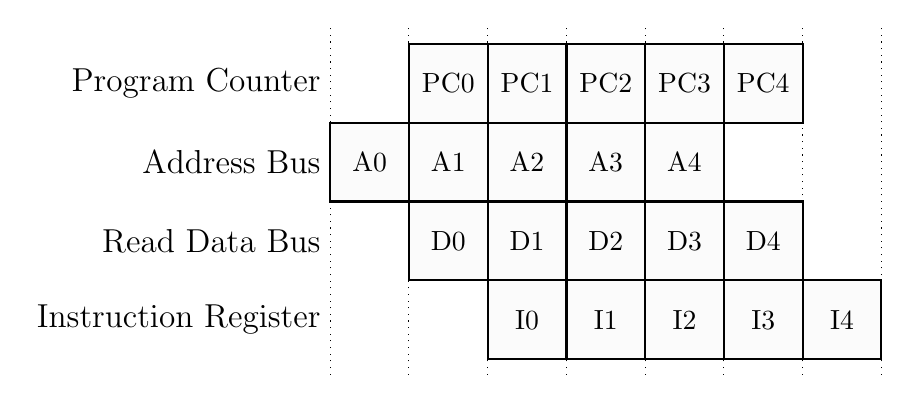
\begin{tikzpicture}

        %Lines
        \draw [dotted] (0,0.3) -- (0,4.7);
        \draw [dotted] (1,0.3) -- (1,4.7);
        \draw [dotted] (2,0.3) -- (2,4.7);
        \draw [dotted] (3,0.3) -- (3,4.7);
        \draw [dotted] (4,0.3) -- (4,4.7);
        \draw [dotted] (5,0.3) -- (5,4.7);
        \draw [dotted] (6,0.3) -- (6,4.7);
        \draw [dotted] (7,0.3) -- (7,4.7);

        %Program counter
        \node  [left] at (0,4) {\large{Program Counter}};
        \draw [thick, fill=gray!3] (1,4.5) rectangle (2,3.5);
        \node at (1.5,4)  {PC0};
        \draw [thick, fill=gray!3] (2,4.5) rectangle (3,3.5);
        \node at (2.5,4)  {PC1};
        \draw [thick, fill=gray!3] (3,4.5) rectangle (4,3.5);
        \node at (3.5,4)  {PC2};
        \draw [thick, fill=gray!3] (4,4.5) rectangle (5,3.5);
        \node at (4.5,4)  {PC3};
        \draw [thick, fill=gray!3] (5,4.5) rectangle (6,3.5);
        \node at (5.5,4)  {PC4};
        
        %Address bus
        \node [left] at (0,3) {\large{Address Bus}};
        \draw [thick, fill=gray!3] (0,3.5) rectangle (1,2.5);
        \node at (0.5,3)  {A0};
        \draw [thick, fill=gray!3] (1,3.5) rectangle (2,2.5);
        \node at (1.5,3)  {A1};
        \draw [thick, fill=gray!3] (2,3.5) rectangle (3,2.5);
        \node at (2.5,3)  {A2};
        \draw [thick, fill=gray!3] (3,3.5) rectangle (4,2.5);
        \node at (3.5,3)  {A3};
        \draw [thick, fill=gray!3] (4,3.5) rectangle (5,2.5);
        \node at (4.5,3)  {A4};

        %Read data bus
        \node [left] at (0,2) {\large{Read Data Bus}};
        \draw [thick, fill=gray!3] (1,2.5) rectangle (2,1.5);
        \node at (1.5,2)  {D0};
        \draw [thick, fill=gray!3] (2,2.5) rectangle (3,1.5);
        \node at (2.5,2)  {D1};
        \draw [thick, fill=gray!3] (3,2.5) rectangle (4,1.5);
        \node at (3.5,2)  {D2};
        \draw [thick, fill=gray!3] (4,2.5) rectangle (5,1.5);
        \node at (4.5,2)  {D3};
        \draw [thick, fill=gray!3] (5,2.5) rectangle (6,1.5);
        \node at (5.5,2)  {D4};

        %Instruction register
        \node [left] at (0,1) {\large{Instruction Register}};
        \draw [thick, fill=gray!3] (2,1.5) rectangle (3,0.5);
        \node at (2.5,1)  {I0};
        \draw [thick, fill=gray!3] (3,1.5) rectangle (4,0.5);
        \node at (3.5,1)  {I1};
        \draw [thick, fill=gray!3] (4,1.5) rectangle (5,0.5);
        \node at (4.5,1)  {I2};
        \draw [thick, fill=gray!3] (5,1.5) rectangle (6,0.5);
        \node at (5.5,1)  {I3};
        \draw [thick, fill=gray!3] (6,1.5) rectangle (7,0.5);
        \node at (6.5,1)  {I4};

      \end{tikzpicture}
    }
  }
  \caption{Plain Linear Execution}
  \label{architecture:excyc:linear:fig}
  \end{center}
\end{figure}


\subsubsection{Execution of Extended Instructions}
\label{architecture:excyc:extended}

In some cases the execution of an instruction can span multiple cycles (i.e. \hyperref[opcodes:ctrl]{non-concurrent control instructions}
or any instruction waiting for a blocked stack access). 
\figref{architecture:excyc:extended:fig} illustrates the timing in these scenarios.

Whenever an opcode needs to be captured from the read data bus, but the instruction register is blocked by an instruction spaning multiple cycles,
The incoming opcode needs to be temourarely stashed away in a separate register.
When the execution of the ongoing instruction is finished, the stashed opcode is moved into the instruction register.

\begin{figure}[!h]
  \begin{center}
  \makebox[\textwidth][c]{
  \scalebox{1} {
      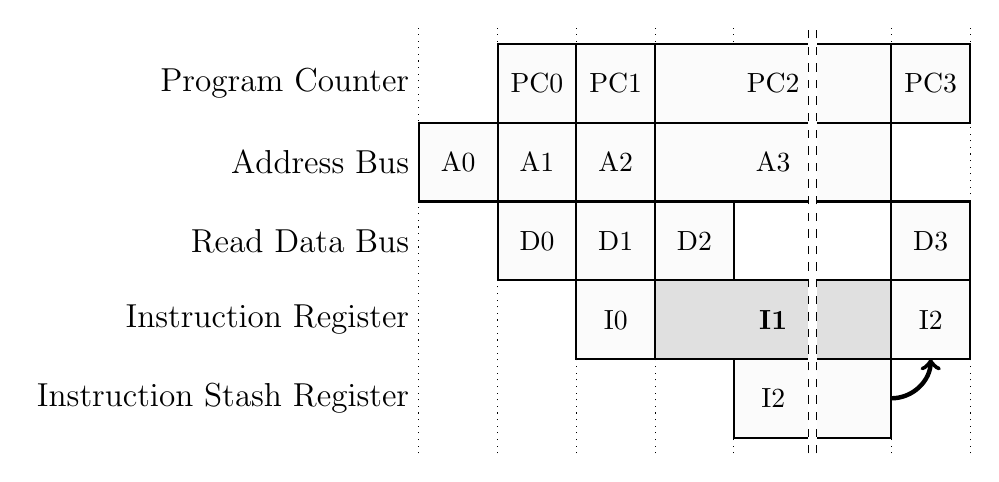
\begin{tikzpicture}

        %Lines
        \draw [dotted] (0,-0.7) -- (0,4.7);
        \draw [dotted] (1,-0.7) -- (1,4.7);
        \draw [dotted] (2,-0.7) -- (2,4.7);
        \draw [dotted] (3,-0.7) -- (3,4.7);
        \draw [dotted] (4,-0.7) -- (4,4.7);
        %\draw [dotted] (5,-0.7) -- (5,4.7);
        \draw [dotted] (6,-0.7) -- (6,4.7);
        \draw [dotted] (7,-0.7) -- (7,4.7);

        %Program counter
        \node  [left] at (0,4) {\large{Program Counter}};
        \draw [thick, fill=gray!3] (1,4.5) rectangle (2,3.5);
        \node at (1.5,4)  {PC0};
        \draw [thick, fill=gray!3] (2,4.5) rectangle (3,3.5);
        \node at (2.5,4)  {PC1};
        \draw [thick, fill=gray!3] (3,4.5) rectangle (6,3.5);
        \node  at (4.5,4)  {PC2};
        \draw [thick, fill=gray!3] (6,4.5) rectangle (7,3.5);
        \node at (6.5,4)  {PC3};
        
        %Address bus
        \node [left] at (0,3) {\large{Address Bus}};
        \draw [thick, fill=gray!3] (0,3.5) rectangle (1,2.5);
        \node at (0.5,3)  {A0};
        \draw [thick, fill=gray!3] (1,3.5) rectangle (2,2.5);
        \node at (1.5,3)  {A1};
        \draw [thick, fill=gray!3] (2,3.5) rectangle (3,2.5);
        \node at (2.5,3)  {A2};
        \draw [thick, fill=gray!3] (3,3.5) rectangle (6,2.5);
        \node at (4.5,3)  {A3};

        %Read data bus
        \node [left] at (0,2) {\large{Read Data Bus}};
        \draw [thick, fill=gray!3] (1,2.5) rectangle (2,1.5);
        \node at (1.5,2)  {D0};
        \draw [thick, fill=gray!3] (2,2.5) rectangle (3,1.5);
        \node at (2.5,2)  {D1};
        \draw [thick, fill=gray!3] (3,2.5) rectangle (4,1.5);
        \node at (3.5,2)  {D2};
        \draw [thick, fill=gray!3] (6,2.5) rectangle (7,1.5);
        \node at (6.5,2)  {D3};

        %Instruction register
        \node [left] at (0,1) {\large{Instruction Register}};
        \draw [thick, fill=gray!3] (2,1.5) rectangle (3,0.5);
        \node at (2.5,1)  {I0};
        \draw [thick, fill=gray!24] (3,1.5) rectangle (6,0.5);
        \node at (4.5,1)  {\textbf{I1}};
        \draw [thick, fill=gray!3] (6,1.5) rectangle (7,0.5);
        \node at (6.5,1)  {I2};

        %Instruction stashregister
        \node [left] at (0,0) {\large{Instruction Stash Register}};
        \draw [thick, fill=gray!3] (4,0.5) rectangle (6,-0.5);
        \node at (4.5,0)  {I2};
        %\draw [ultra thick, ->]  (5,0) -- (5.5,0) -- (5.5,0.5);
        \draw [ultra thick, ->] (6,0) arc (270:360:0.5) ;

        %Gap
        %\draw [dotted] (5,-0.7) -- (5,4.7);
        \draw [fill=white, white] (4.95,-0.7) rectangle (5.05,4.7);
        \draw [dashed] (4.95,-0.7) -- (4.95,4.7);
        \draw [dashed] (5.05,-0.7) -- (5.05,4.7);

        
      \end{tikzpicture}
    }
  }
  \caption{Execution of an Extended Instruction}
  \label{architecture:excyc:extended:fig}
  \end{center}
\end{figure}


\subsubsection{Execution of Memory Access Instructions}
\label{architecture:excyc:mem}

A special case of multi-cycle instructions are \hyperref[opcodes:memacc]{memory access instructions}.
These instructions perform their memory acesses on the program bus.
\figref{architecture:excyc:mem:fig} illustrates how opcode fetches and data accesses are interleaved.

\begin{figure}[!h]
  \begin{center}
  \makebox[\textwidth][c]{
  \scalebox{1} {
      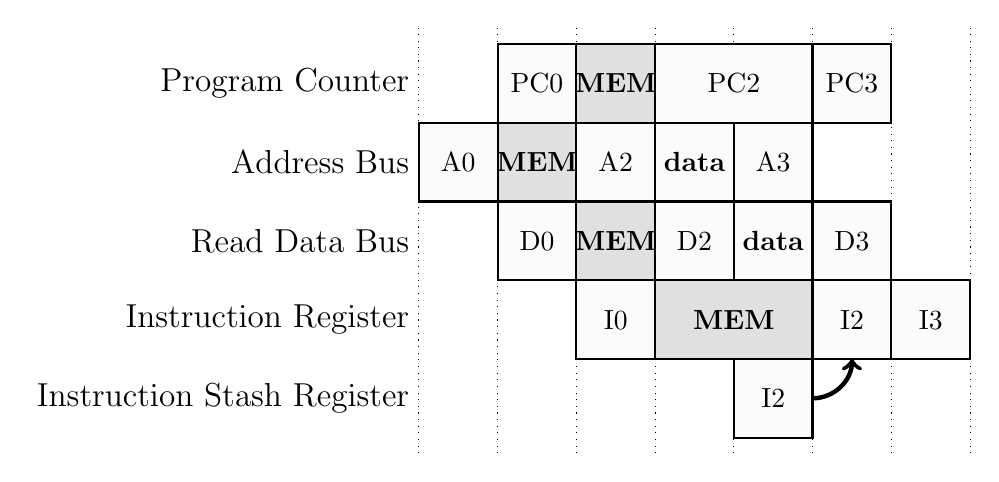
\begin{tikzpicture}

        %Lines
        \draw [dotted] (0,-0.7) -- (0,4.7);
        \draw [dotted] (1,-0.7) -- (1,4.7);
        \draw [dotted] (2,-0.7) -- (2,4.7);
        \draw [dotted] (3,-0.7) -- (3,4.7);
        \draw [dotted] (4,-0.7) -- (4,4.7);
        \draw [dotted] (5,-0.7) -- (5,4.7);
        \draw [dotted] (6,-0.7) -- (6,4.7);
        \draw [dotted] (7,-0.7) -- (7,4.7);

        %Program counter
        \node  [left] at (0,4) {\large{Program Counter}};
        \draw [thick, fill=gray!3] (1,4.5) rectangle (2,3.5);
        \node at (1.5,4)  {PC0};
        \draw [thick, fill=gray!24] (2,4.5) rectangle (3,3.5);
        \node at (2.5,4)  {\textbf{MEM}};
        \draw [thick, fill=gray!3] (3,4.5) rectangle (5,3.5);
        \node  at (4,4)  {PC2};
        \draw [thick, fill=gray!3] (5,4.5) rectangle (6,3.5);
        \node at (5.5,4)  {PC3};
        
        %Address bus
        \node [left] at (0,3) {\large{Address Bus}};
        \draw [thick, fill=gray!3] (0,3.5) rectangle (1,2.5);
        \node at (0.5,3)  {A0};
        \draw [thick, fill=gray!24] (1,3.5) rectangle (2,2.5);
        \node at (1.5,3)  {\textbf{MEM}};
        \draw [thick, fill=gray!3] (2,3.5) rectangle (3,2.5);
        \node at (2.5,3)  {A2};
        \draw [thick, fill=gray!3] (3,3.5) rectangle (4,2.5);
        \node at (3.5,3)  {\textbf{data}};
        \draw [thick, fill=gray!3] (4,3.5) rectangle (5,2.5);
        \node at (4.5,3)  {A3};

        %Read data bus
        \node [left] at (0,2) {\large{Read Data Bus}};
        \draw [thick, fill=gray!3] (1,2.5) rectangle (2,1.5);
        \node at (1.5,2)  {D0};
        \draw [thick, fill=gray!24] (2,2.5) rectangle (3,1.5);
        \node at (2.5,2)  {\textbf{MEM}};
        \draw [thick, fill=gray!3] (3,2.5) rectangle (4,1.5);
        \node at (3.5,2)  {D2};
        \draw [thick, fill=gray!3] (4,2.5) rectangle (5,1.5);
        \node at (4.5,2)  {\textbf{data}};
        \draw [thick, fill=gray!3] (5,2.5) rectangle (6,1.5);
        \node at (5.5,2)  {D3};

        %Instruction register
        \node [left] at (0,1) {\large{Instruction Register}};
        \draw [thick, fill=gray!3] (2,1.5) rectangle (3,0.5);
        \node at (2.5,1)  {I0};
        \draw [thick, fill=gray!24] (3,1.5) rectangle (5,0.5);
        \node at (4,1)  {\textbf{MEM}};
        \draw [thick, fill=gray!3] (5,1.5) rectangle (6,0.5);
        \node at (5.5,1)  {I2};
        \draw [thick, fill=gray!3] (6,1.5) rectangle (7,0.5);
        \node at (6.5,1)  {I3};

        %Instruction stash register
        \node [left] at (0,0) {\large{Instruction Stash Register}};
        \draw [thick, fill=gray!3] (4,0.5) rectangle (5,-0.5);
        \node at (4.5,0)  {I2};
        %\draw [ultra thick, ->]  (5,0) -- (5.5,0) -- (5.5,0.5);
        \draw [ultra thick, ->] (5,0) arc (270:360:0.5) ;

      \end{tikzpicture}
    }
  }
  \caption{Execution of a Memory Access Instruction}
  \label{architecture:excyc:mem:fig}
  \end{center}
\end{figure}


\subsubsection{Change of Flow Instructions}
\label{architecture:excyc:cof}

%Change of flow instructions
TBD

\begin{figure}[!h]
  \begin{center}
  \makebox[\textwidth][c]{
  \scalebox{1} {
      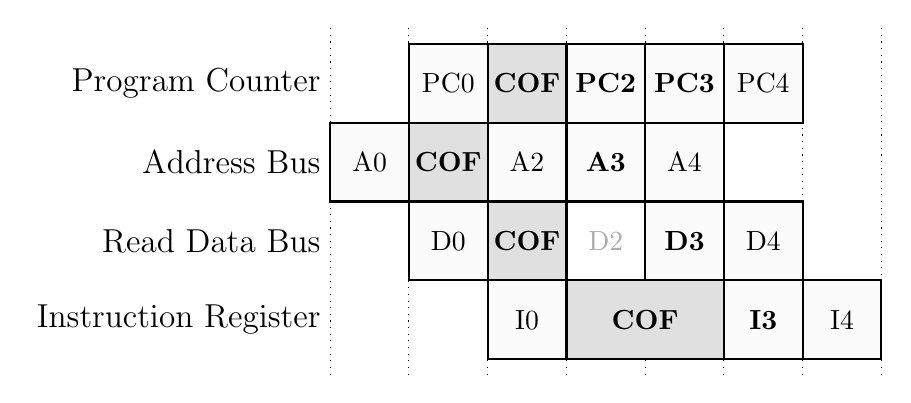
\begin{tikzpicture}

        %Lines
        \draw [dotted] (0,0.3) -- (0,4.7);
        \draw [dotted] (1,0.3) -- (1,4.7);
        \draw [dotted] (2,0.3) -- (2,4.7);
        \draw [dotted] (3,0.3) -- (3,4.7);
        \draw [dotted] (4,0.3) -- (4,4.7);
        \draw [dotted] (5,0.3) -- (5,4.7);
        \draw [dotted] (6,0.3) -- (6,4.7);
        \draw [dotted] (7,0.3) -- (7,4.7);

        %Program counter
        \node  [left] at (0,4) {\large{Program Counter}};
        \draw [thick, fill=gray!3] (1,4.5) rectangle (2,3.5);
        \node at (1.5,4)  {PC0};
        \draw [thick, fill=gray!24] (2,4.5) rectangle (3,3.5);
        \node at (2.5,4)  {\textbf{COF}};
        \draw [thick, fill=gray!3] (3,4.5) rectangle (4,3.5);
        \node at (3.5,4)  {\textbf{PC2}};
        \draw [thick, fill=gray!3] (4,4.5) rectangle (5,3.5);
        \node at (4.5,4)  {\textbf{PC3}};
        \draw [thick, fill=gray!3] (5,4.5) rectangle (6,3.5);
        \node at (5.5,4)  {PC4};
        
        %Address bus
        \node [left] at (0,3) {\large{Address Bus}};
        \draw [thick, fill=gray!3] (0,3.5) rectangle (1,2.5);
        \node at (0.5,3)  {A0};
        \draw [thick, fill=gray!24] (1,3.5) rectangle (2,2.5);
        \node at (1.5,3)  {\textbf{COF}};
        \draw [thick, fill=gray!3] (2,3.5) rectangle (3,2.5);
        \node at (2.5,3)  {A2};
        \draw [thick, fill=gray!3] (3,3.5) rectangle (4,2.5);
        \node at (3.5,3)  {\textbf{A3}};
        \draw [thick, fill=gray!3] (4,3.5) rectangle (5,2.5);
        \node at (4.5,3)  {A4};

        %Read data bus
        \node [left] at (0,2) {\large{Read Data Bus}};
        \draw [thick, fill=gray!3] (1,2.5) rectangle (2,1.5);
        \node at (1.5,2)  {D0};
        \draw [thick, fill=gray!24] (2,2.5) rectangle (3,1.5);
        \node at (2.5,2)  {\textbf{COF}};
        \draw [thick] (3,2.5) rectangle (4,1.5);
        \node [text=gray!64] at (3.5,2)  {D2};
        \draw [thick, fill=gray!3] (4,2.5) rectangle (5,1.5);
        \node at (4.5,2)  {\textbf{D3}};
        \draw [thick, fill=gray!3] (5,2.5) rectangle (6,1.5);
        \node at (5.5,2)  {D4};

        %Instruction register
        \node [left] at (0,1) {\large{Instruction Register}};
        \draw [thick, fill=gray!3] (2,1.5) rectangle (3,0.5);
        \node at (2.5,1)  {I0};
        \draw [thick, fill=gray!24] (3,1.5) rectangle (5,0.5);
        \node at (4,1)  {\textbf{COF}};
        \draw [thick, fill=gray!3] (5,1.5) rectangle (6,0.5);
        \node at (5.5,1)  {\textbf{I3}};
        \draw [thick, fill=gray!3] (6,1.5) rectangle (7,0.5);
        \node at (6.5,1)  {I4};

      \end{tikzpicture}
    }
  }
  \caption{Execution of a Change of Flow Instruction}
  \label{architecture:excyc:cof:fig}
  \end{center}
\end{figure}


\subsubsection{Exceptions and Interrupts}
\label{architecture:excyc:excpt}

%Exceptions
TBD

\begin{figure}[!h]
  \begin{center}
  \makebox[\textwidth][c]{
  \scalebox{1} {
      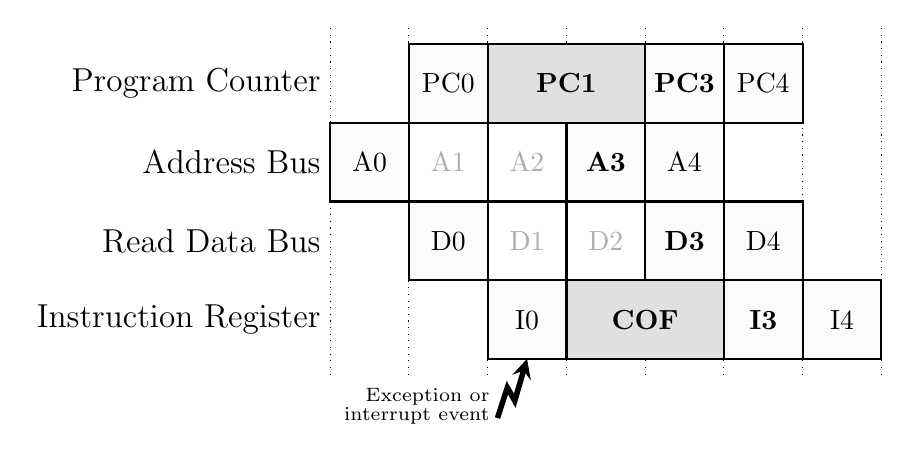
\begin{tikzpicture}

        %Lines
        \draw [dotted] (0,0.3) -- (0,4.7);
        \draw [dotted] (1,0.3) -- (1,4.7);
        \draw [dotted] (2,0.3) -- (2,4.7);
        \draw [dotted] (3,0.3) -- (3,4.7);
        \draw [dotted] (4,0.3) -- (4,4.7);
        \draw [dotted] (5,0.3) -- (5,4.7);
        \draw [dotted] (6,0.3) -- (6,4.7);
        \draw [dotted] (7,0.3) -- (7,4.7);

        %Program counter
        \node  [left] at (0,4) {\large{Program Counter}};
        \draw [thick, fill=gray!3] (1,4.5) rectangle (2,3.5);
        \node at (1.5,4)  {PC0};
        \draw [thick, fill=gray!24] (2,4.5) rectangle (4,3.5);
        \node at (3,4)  {\textbf{PC1}};
        %\draw [thick] (3,4.5) rectangle (4,3.5);
        %\node [text=gray!64] at (3.5,4)  {PC1};
        \draw [thick, fill=gray!3] (4,4.5) rectangle (5,3.5);
        \node at (4.5,4)  {\textbf{PC3}};
        \draw [thick, fill=gray!3] (5,4.5) rectangle (6,3.5);
        \node at (5.5,4)  {PC4};
        
        %Address bus
        \node [left] at (0,3) {\large{Address Bus}};
        \draw [thick, fill=gray!3] (0,3.5) rectangle (1,2.5);
        \node at (0.5,3)  {A0};1
        \draw [thick] (1,3.5) rectangle (2,2.5);
        \node [text=gray!64] at (1.5,3)  {A1};
        \draw [thick] (2,3.5) rectangle (3,2.5);
        \node [text=gray!64]  at (2.5,3)  {A2};
        \draw [thick, fill=gray!3] (3,3.5) rectangle (4,2.5);
        \node at (3.5,3)  {\textbf{A3}};
        \draw [thick, fill=gray!3] (4,3.5) rectangle (5,2.5);
        \node at (4.5,3)  {A4};

        %Read data bus
        \node [left] at (0,2) {\large{Read Data Bus}};
        \draw [thick, fill=gray!3] (1,2.5) rectangle (2,1.5);
        \node at (1.5,2)  {D0};
        \draw [thick] (2,2.5) rectangle (3,1.5);
        \node [text=gray!64] at (2.5,2)  {D1};
        \draw [thick] (3,2.5) rectangle (4,1.5);
        \node [text=gray!64] at (3.5,2)  {D2};
        \draw [thick, fill=gray!3] (4,2.5) rectangle (5,1.5);
        \node at (4.5,2)  {\textbf{D3}};
        \draw [thick, fill=gray!3] (5,2.5) rectangle (6,1.5);
        \node at (5.5,2)  {D4};

        %Instruction register
        \node [left] at (0,1) {\large{Instruction Register}};
        \draw [thick, fill=gray!3] (2,1.5) rectangle (3,0.5);
        \node at (2.5,1)  {I0};
        \draw [thick, fill=gray!24] (3,1.5) rectangle (5,0.5);
        \node at (4,1)  {\textbf{COF}};
        \draw [thick, fill=gray!3] (5,1.5) rectangle (6,0.5);
        \node at (5.5,1)  {\textbf{I3}};
        \draw [thick, fill=gray!3] (6,1.5) rectangle (7,0.5);
        \node at (6.5,1)  {I4};

        %Exception
        \draw [line width=2pt,-stealth] (2.125,-0.25) -- (2.25,0.135) -- (2.34375,-0.03125) -- (2.5,0.5);
        \node [align=right] at (1.1,-0.1) {\scriptsize{Exception or} \\[-5pt] \scriptsize{interrupt event}};

        
      \end{tikzpicture}
    }
  }
  \caption{Program flow interruted by an exception - TBD}
  \label{architecture:excyc:excpt:fig}
  \end{center}
\end{figure}


\subsection{Design Components}
\label{architecture:comp}

The N1 architecture is divided in 11 subblocks as shown in \figref{architecture:comp:fig}.

\begin{figure}[!h]
  \begin{center}
  \makebox[\textwidth][c]{
  \scalebox{1} {
      
\begin{tikzpicture}

        \node [left] at (0,0) {\large{TBD}};

      \end{tikzpicture}
    }
  }
  \caption{Block Diagram}
  \label{architecture:comp:fig}
  \end{center}
\end{figure}


\subsubsection{Flow Control Block (\texttt{fc})}
\label{architecture:fc}

The flow control block is implemented in the Verilog module \texttt{N1\_fc} (N1\_fc.v).
It manages the  \hyperref[architecture:excyc]{instruction cycles} of the N1 core.
It handles the control and resonse signals of the  \hyperref[integration:if:pbus]{program bus's} \gls{wb} interface and
it communicates with the other N1 componenents by sending requests and receiving status information.
No actual data passes through the \texttt{N1\_fc} module.
The interfaces to the N1 compunents, which are under the control of the flow control block, are explained in the following sections.

\paragraph{Control and Status Interface to the \hyperref[architecture:comp:ir]{Instruction Register}} \mbox{} \\
\label{architecture:fc:irif}

The flow control block is able to request has the following request signals to the instruction register: 
\begin{description}[style=nextline]

\item[\texttt{fc2ir\_capture}]
Capture the \hyperref[integration:if:pbus]{program bus's} read data (\texttt{pbus\_dat\_i}) in the
instruction register at the next clock edge.

\item[\texttt{fc2ir\_stash}]
Capture the \hyperref[integration:if:pbus]{program bus's} read data (\texttt{pbus\_dat\_i}) in the
stash register at the next clock edge.

\item[\texttt{fc2ir\_expend}]
The read data input of the \hyperref[integration:if:pbus]{Program Bus (\texttt{pbus\_dat\_i})}

\item[\texttt{fc2ir\_expend}]
Copy the stash regiesr's content into the instruction register at the next clock cycle.

\end{description}

The following status signala are coming from the instruction register:
%\begin{description}[style=nextline]
%\end{description}


\subsubsection{Instruction Register (\texttt{ir})}
\label{architecture:comp:ir}







%\subsubsection{Incoming Information}
%\label{architecture:ir:in}
%
%\subsubsection{Outgoing Information}
%\label{architecture:ir:out}

\subsubsection{Arithmetic Logic Unit (\texttt{alu})}
\label{architecture:comp:alu}

TBD

%\subsubsection{Incoming Information}
%\label{architecture:alu:in}

%\subsubsection{Outgoing Information}
%\label{architecture:alu:out}

\subsubsection{DSP Block (\texttt{dsp})}
\label{architecture:comp:dsp}

TBD

%\subsubsection{Incoming Information}
%\label{architecture:alu:in}

%\subsubsection{Outgoing Information}
%\label{architecture:alu:out}

\subsubsection{Exception Handler (\texttt{excpt})}
\label{architecture:comp:excpt}

TBD

%\subsubsection{Incoming Information}
%\label{architecture:alu:in}

%\subsubsection{Outgoing Information}
%\label{architecture:alu:out}

\subsubsection{Upper Stack (\texttt{us})}
\label{architecture:comp:us}

TBD

%\subsubsection{Incoming Information}
%\label{architecture:us:in}

%\subsubsection{Outgoing Information}
%\label{architecture:us:out}

\subsubsection{Intermediate Parameter Stack (\texttt{ips})}
\label{architecture:comp:ips}

TBD

%\subsubsection{Incoming Information}
%\label{architecture:ips:in}

%\subsubsection{Outgoing Information}
%\label{architecture:ips:out}

\subsubsection{Intermediate Return Stack (\texttt{irs})}
\label{architecture:comp:irs}

TBD

%\subsubsection{Incoming Information}
%\label{architecture:irs:in}

%\subsubsection{Outgoing Information}
%\label{architecture:irs:out}

\subsubsection{Lower Stack (\texttt{ls})}
\label{architecture:comp:ls}

TBD

%\subsubsection{Incoming Information}
%\label{architecture:ls:in}

%\subsubsection{Outgoing Information}
%\label{architecture:ls:out}



%--------------------
% Verification 
%--------------------
%###############################################################################
%# N1 - Manual - Verification Status                                           #
%###############################################################################
%#    Copyright 2018 - 2019 Dirk Heisswolf                                     #
%#    This file is part of the N1 project.                                     #
%#                                                                             #
%#    N1 is free software: you can redistribute it and/or modify               #
%#    it under the terms of the GNU General Public License as published by     #
%#    the Free Software Foundation, either version 3 of the License, or        #
%#    (at your option) any later version.                                      #
%#                                                                             #
%#    N1 is distributed in the hope that it will be useful,                    #
%#    but WITHOUT ANY WARRANTY; without even the implied warranty of           #
%#    MERCHANTABILITY or FITNESS FOR A PARTICULAR PURPOSE.  See the            #
%#    GNU General Public License for more details.                             #
%#                                                                             #
%#    You should have received a copy of the GNU General Public License        #
%#    along with N1.  If not, see <http://www.gnu.org/licenses/>.              #
%###############################################################################
%# Version History:                                                            #
%#   March 4, 2019                                                             #
%#      - Initial release                                                      #
%###############################################################################

\section{Verification Status}
\label{verification}

TBD



%--------------------
% Tool summary
%--------------------
%###############################################################################
%# N1 - Manual - Tool Summary                                                  #
%###############################################################################
%#    Copyright 2018 - 2019 Dirk Heisswolf                                     #
%#    This file is part of the N1 project.                                     #
%#                                                                             #
%#    N1 is free software: you can redistribute it and/or modify               #
%#    it under the terms of the GNU General Public License as published by     #
%#    the Free Software Foundation, either version 3 of the License, or        #
%#    (at your option) any later version.                                      #
%#                                                                             #
%#    N1 is distributed in the hope that it will be useful,                    #
%#    but WITHOUT ANY WARRANTY; without even the implied warranty of           #
%#    MERCHANTABILITY or FITNESS FOR A PARTICULAR PURPOSE.  See the            #
%#    GNU General Public License for more details.                             #
%#                                                                             #
%#    You should have received a copy of the GNU General Public License        #
%#    along with N1.  If not, see <http://www.gnu.org/licenses/>.              #
%###############################################################################
%# Version History:                                                            #
%#   March 5, 2019                                                             #
%#      - Initial release                                                      #
%###############################################################################

\section{Tool Summary}
\label{tools}

TBD



%--------------------
% Bibliography
%--------------------
\bibliographystyle{plain}
\bibliography{N1.bib}

\end{document}
